\chapter{Results - Person specific}
{\samenvatting todo}

In a later stage research was done to select features that work well in a cross person setting, meaning that the model was trained on one set of persons and then tested on another set, containing different persons. This part is more challenging as physiological signals are very person from nature \ref{DEAPSignals}.

\section{Approach}

To do so, the approach from Section \ref{approach} was modified slightly. The only difference is that the splits in test and train set as well as the cross validation was based on persons. This means that once a single sample from a person is placed in a set, all his other samples are added as well. Special care was taken to ensure that the random forest would also work correctly. The problem with random forest is that they create an out of bag sample, as explained in Section \ref{rfexpl}. Because this out of bag sample is used as a validation set, a custom random forest was created. This random forest would split the out of bag sample based on the different persons.

\section{Performance}
The performance of the different algorithms is depicted in Figure \ref{accComp_arousalSVM_gen} for arousal and Figure \ref{accComp_valenceSVM_gen} for valence. The legend, combined with an overview of the accuracy values is given in Table \ref{genacctable}. As you can see the performance in a cross subject setting is much lower. This is due to the personal aspect of physiological signals. These results are not surprising, when considering that a person specific classifier achieves a maximal accuracy around 70\%. Going from a person specific to a cross person classifier, corresponds to a drop in performance, as the physiological features are person specific. Improving the accuracy in a cross subject setting might be a topic for future research. 

\begin{table}[H]
\centering
\begin{tabular}{llll}
\textbf{Number} & \textbf{feature selection method} & \textbf{avg test acc - arousal} & \textbf{avg test acc - valence} \\
0               & pearsonR                          & 0.62187                             & 0.51875                             \\
1               & MutInf                            & 0.59688                             & 0.56563                             \\
2               & dCorr                             & 0.58125                             & 0.51875                             \\
3               & LR                                & 0.61562                             & 0.55312                             \\
4               & L1                                & 0.59688                             & 0.55312                             \\
5               & L2                                & 0.58125                             & 0.55937                             \\
6               & SVM                               & 0.60938                             & 0.5375                              \\
7               & RF                                & 0.63438                             & 0.55312                             \\
8               & ANOVA                             & 0.60312                             & 0.53438                             \\
9               & LDA                               & 0.63438                             & 0.52812                             \\
10              & PCA                               & 0.62187                             & 0.5375                             
\end{tabular}
\caption{The different feature selection methods and their labels\label{genacctable}.}
\end{table}

\mijnfiguur{width=1.\textwidth}{accComp_arousalSVM_gen}{Comparison of different feature selection methods for arousal recognition in a cross subject setting. The blue bars correspond to filter selection methods. Red bars correspond to wrapper methods and green bars are used for the embedded methods.}

\mijnfiguur{width=1.\textwidth}{accComp_valenceSVM_gen}{Comparison of different feature selection methods for valence recognition in a cross subject setting. The blue bars correspond to filter selection methods. Red bars correspond to wrapper methods and green bars are used for the embedded methods.}

\section{Correlation probability and level of valence/arousal}
TODO
%TODO

\section{Selected features}

To compare which features where chosen, the feature set was, again divided into 9 categories:
\begin{enumerate}
\item \textbf{Power features:} PSD and FE features of a single channel
\item \textbf{Asymmetry features:} DASM, RASM, DCAU and RCAU features that represent a the (a)symmetry between two channels.
\item \textbf{Fractions:} Alpha/beta and fractions of different power ratios of a channels.

\item \textbf{Heart rate:} the statistical values of the heart rate.
\item \textbf{Galvanic skin response:} the statistical values of the GSR.
\item \textbf{Respiration:} the statistical values of the respiration.
\item \textbf{Bloop pressure:} the statistical values of the plethysmograph.
\item \textbf{Skin temp:} the statistical values of the skin temperature.
\end{enumerate} 

The selected features are depicted in Figure \ref{arousalpiesgen} and \ref{valencepiesgen} for arousal and valence respectively.

\clearpage
\begin{figure}[!tbp]
  \centering
  \caption{Selection features for arousal classification.\label{arousalpiesgen}}
  \begin{subfigure}[b]{0.3\textwidth}
    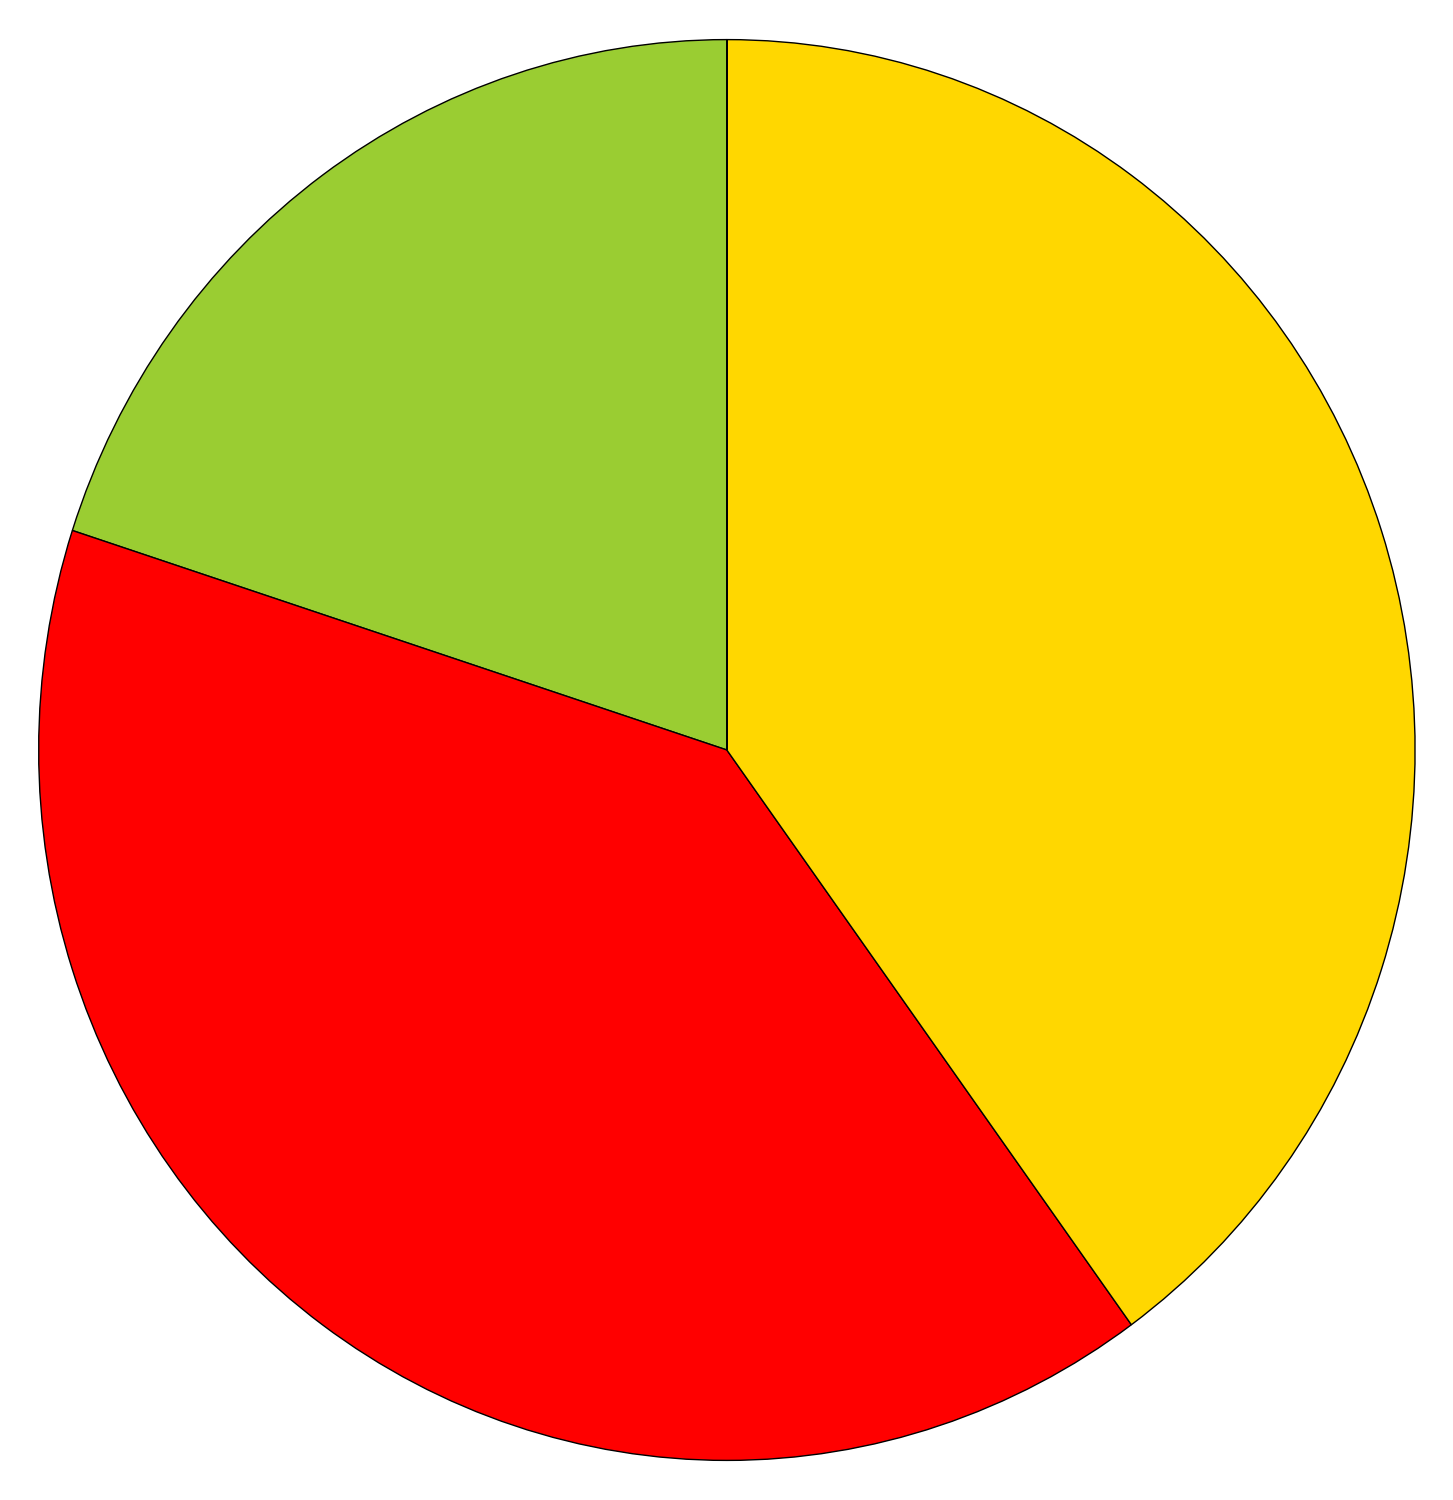
\includegraphics[width=\textwidth]{arousalALLpearsonRgen}
    \caption{Pearson correlation}
  \end{subfigure}
  \hfill
  \begin{subfigure}[b]{0.3\textwidth}
    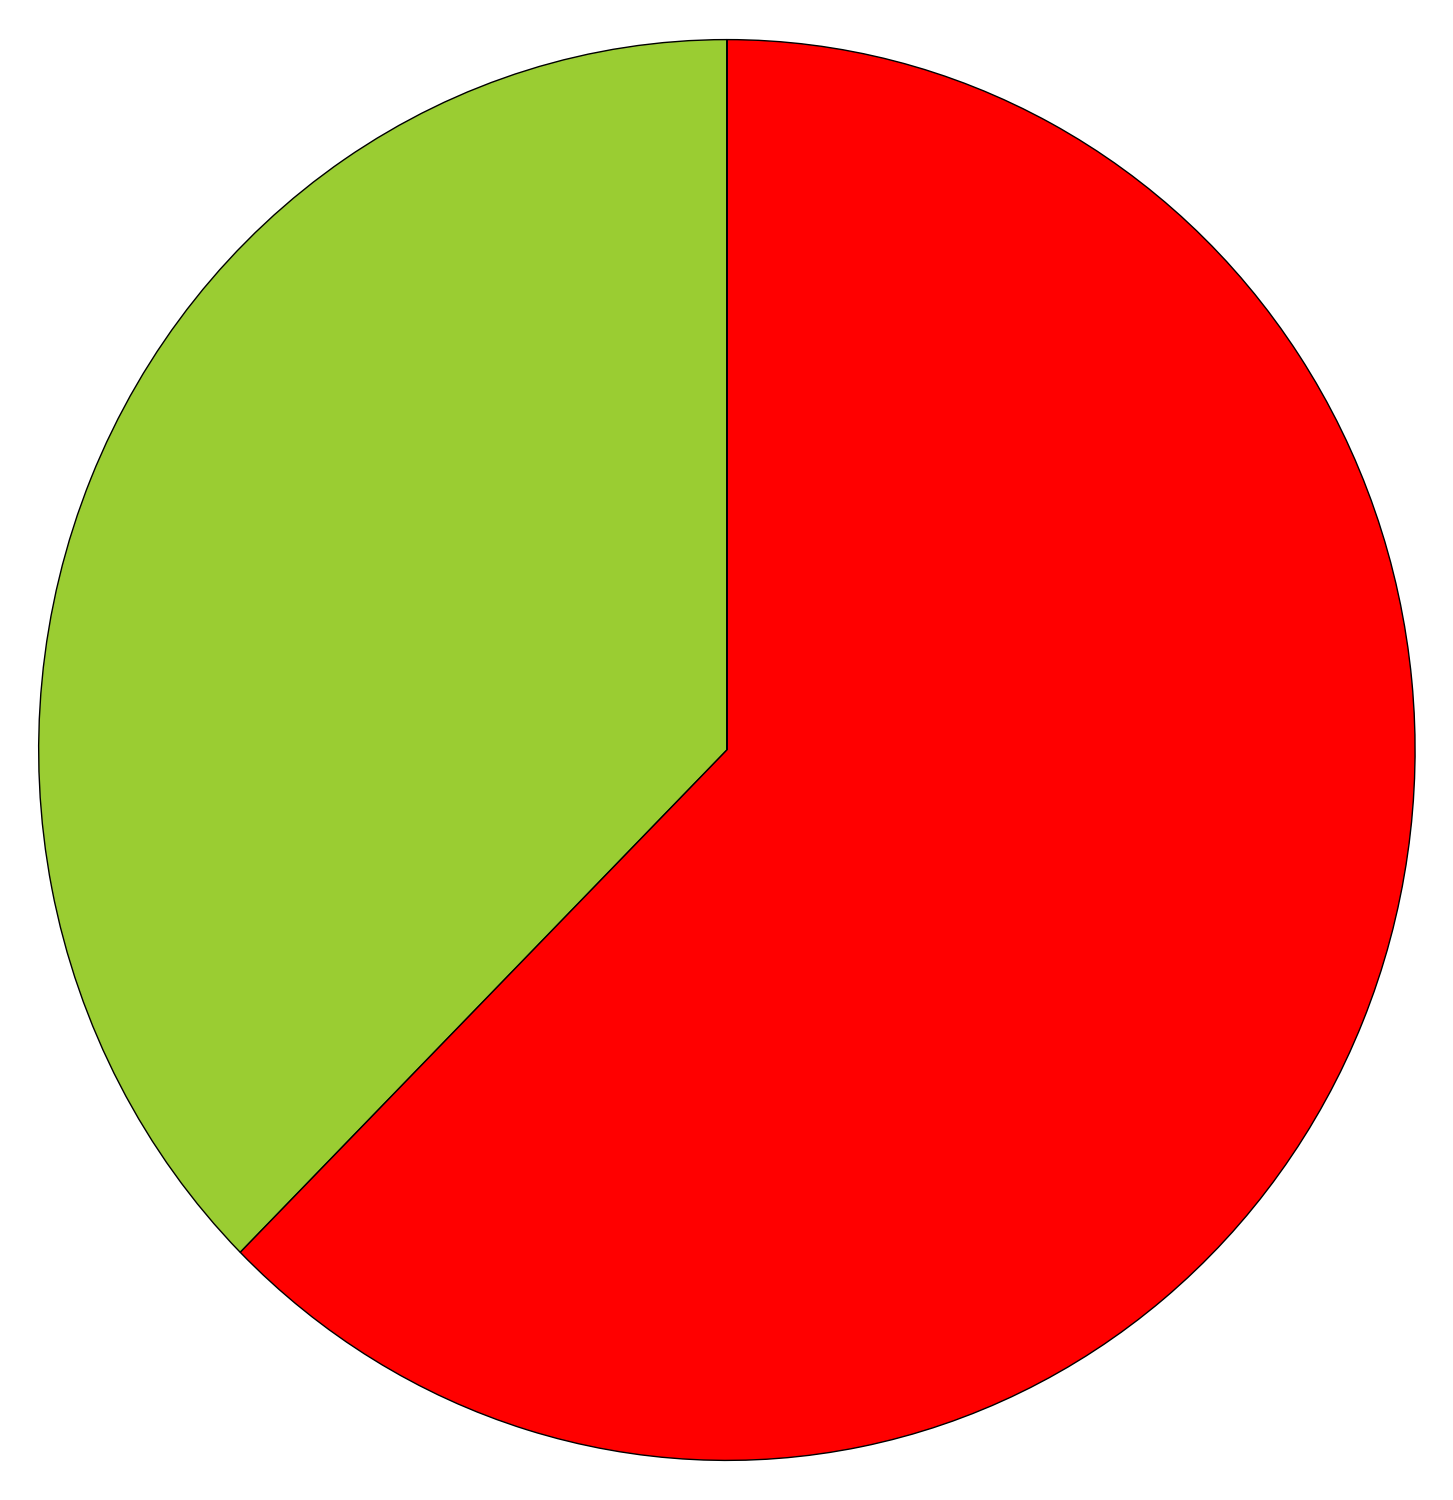
\includegraphics[width=\textwidth]{arousalALLMutInfgen}
    \caption{Mutual information}
  \end{subfigure}
  \hfill
  \begin{subfigure}[b]{0.3\textwidth}
    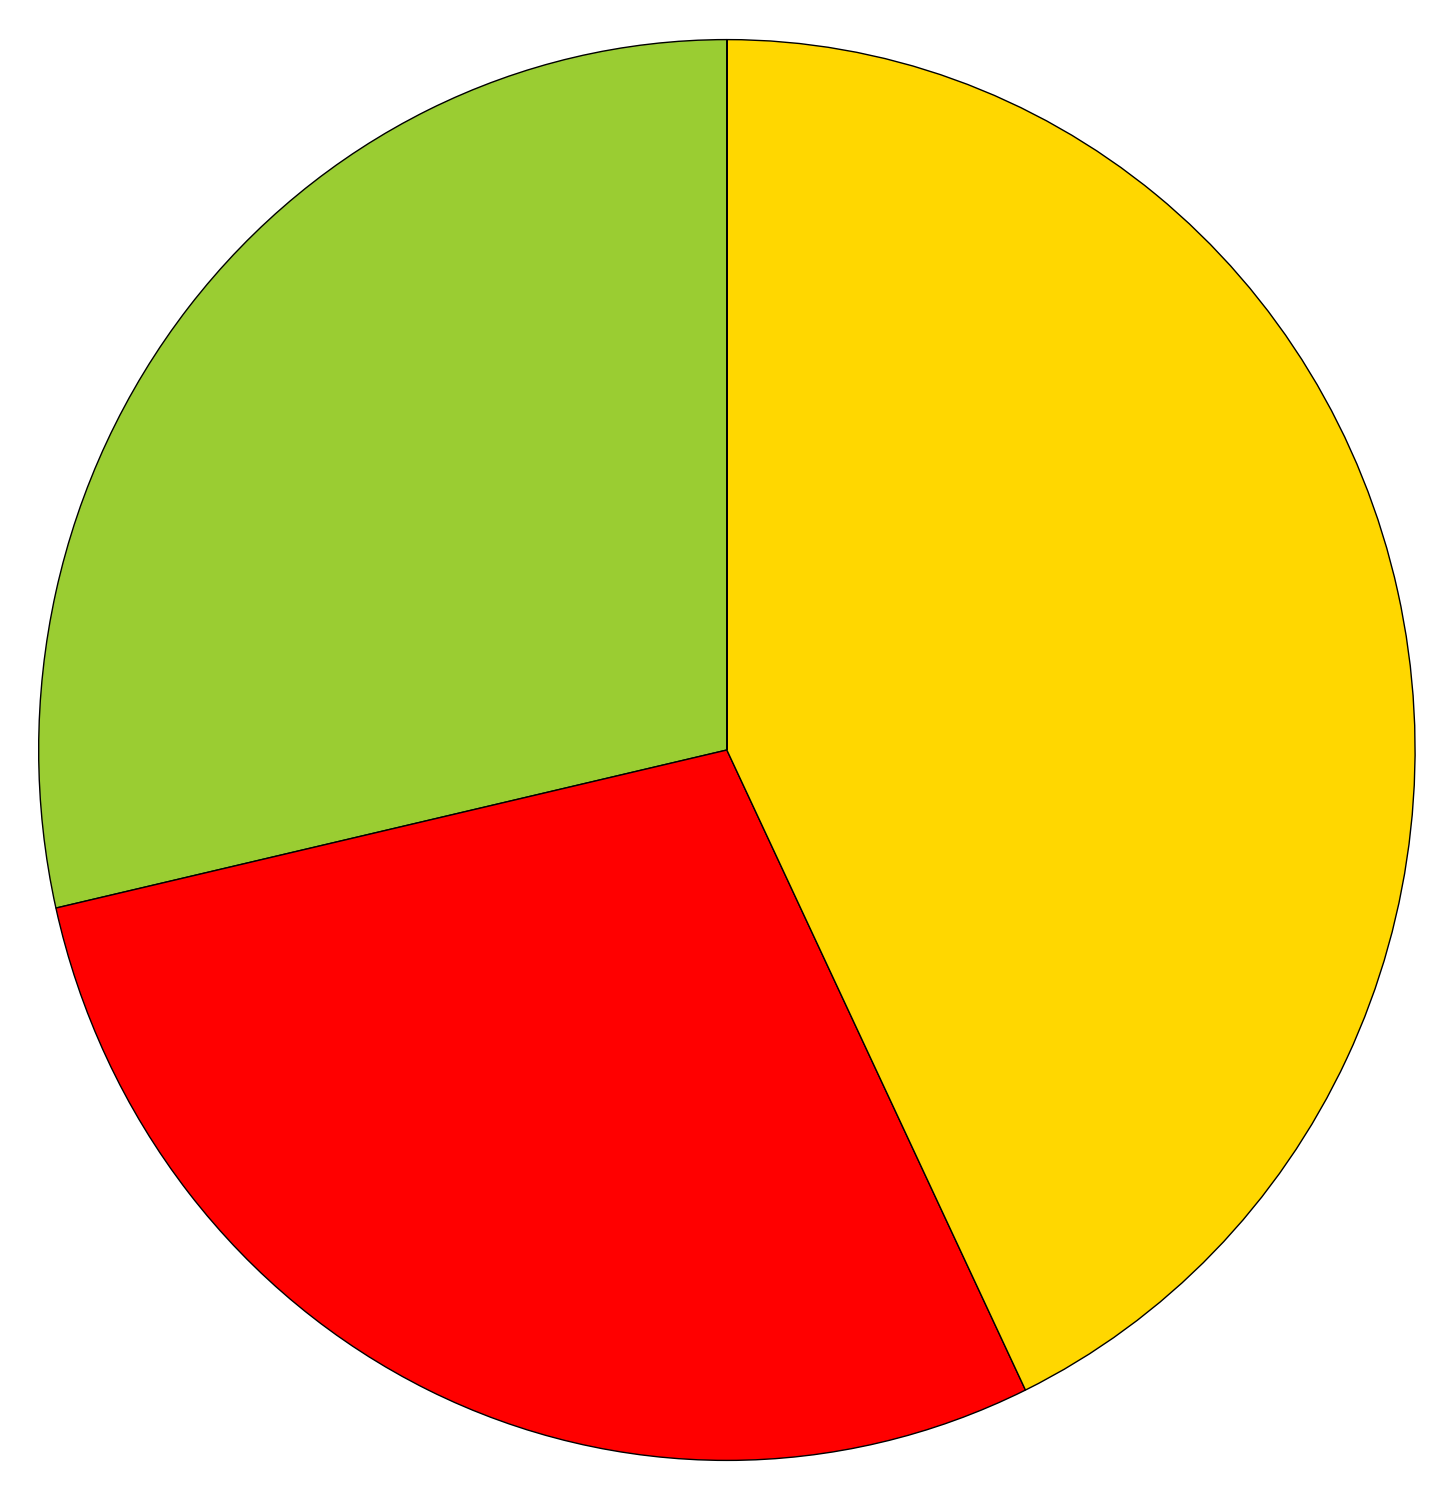
\includegraphics[width=\textwidth]{arousalALLdCorrgen}
    \caption{Distance Correlation}
  \end{subfigure}
  
  \begin{subfigure}[b]{0.3\textwidth}
    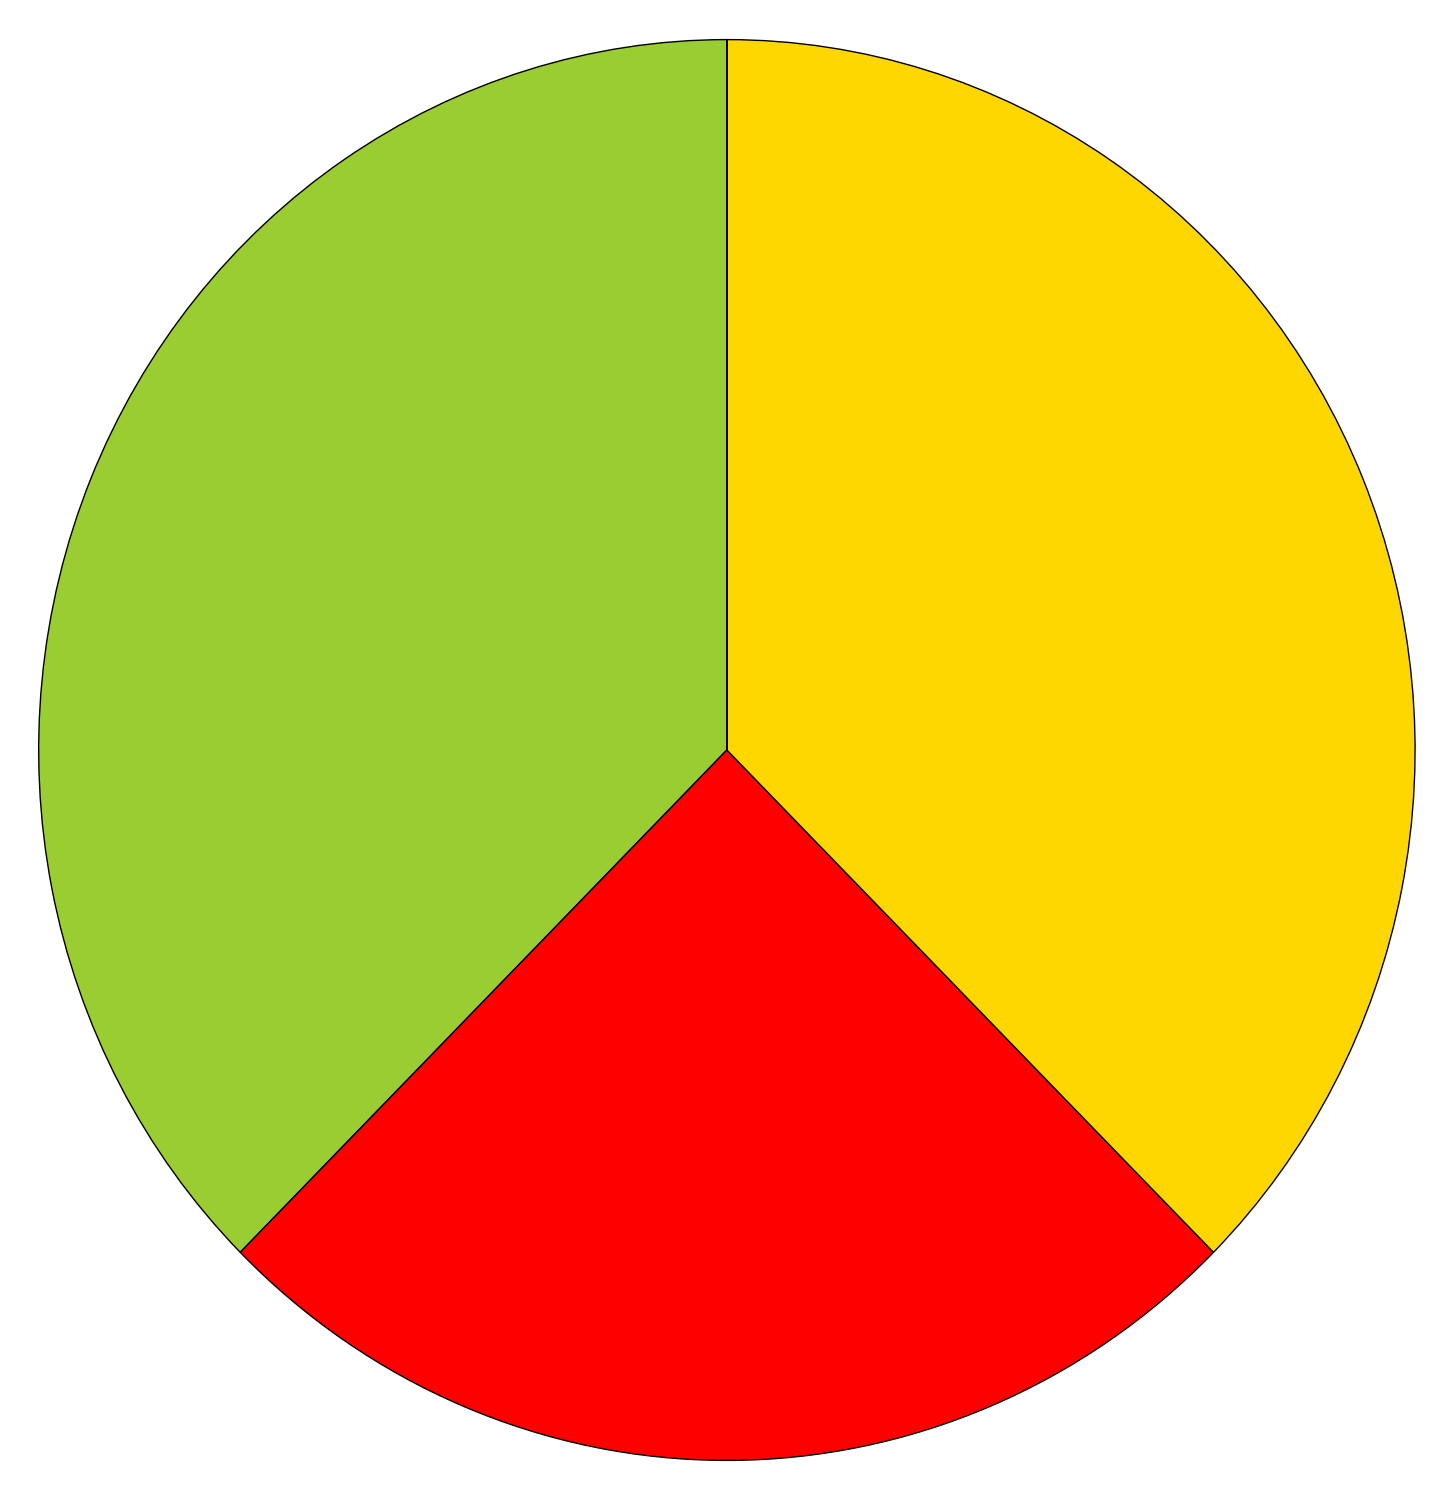
\includegraphics[width=\textwidth]{arousalALLANOVAgen}
    \caption{ANOVA}
  \end{subfigure}
  \hfill
  \begin{subfigure}[b]{0.3\textwidth}
    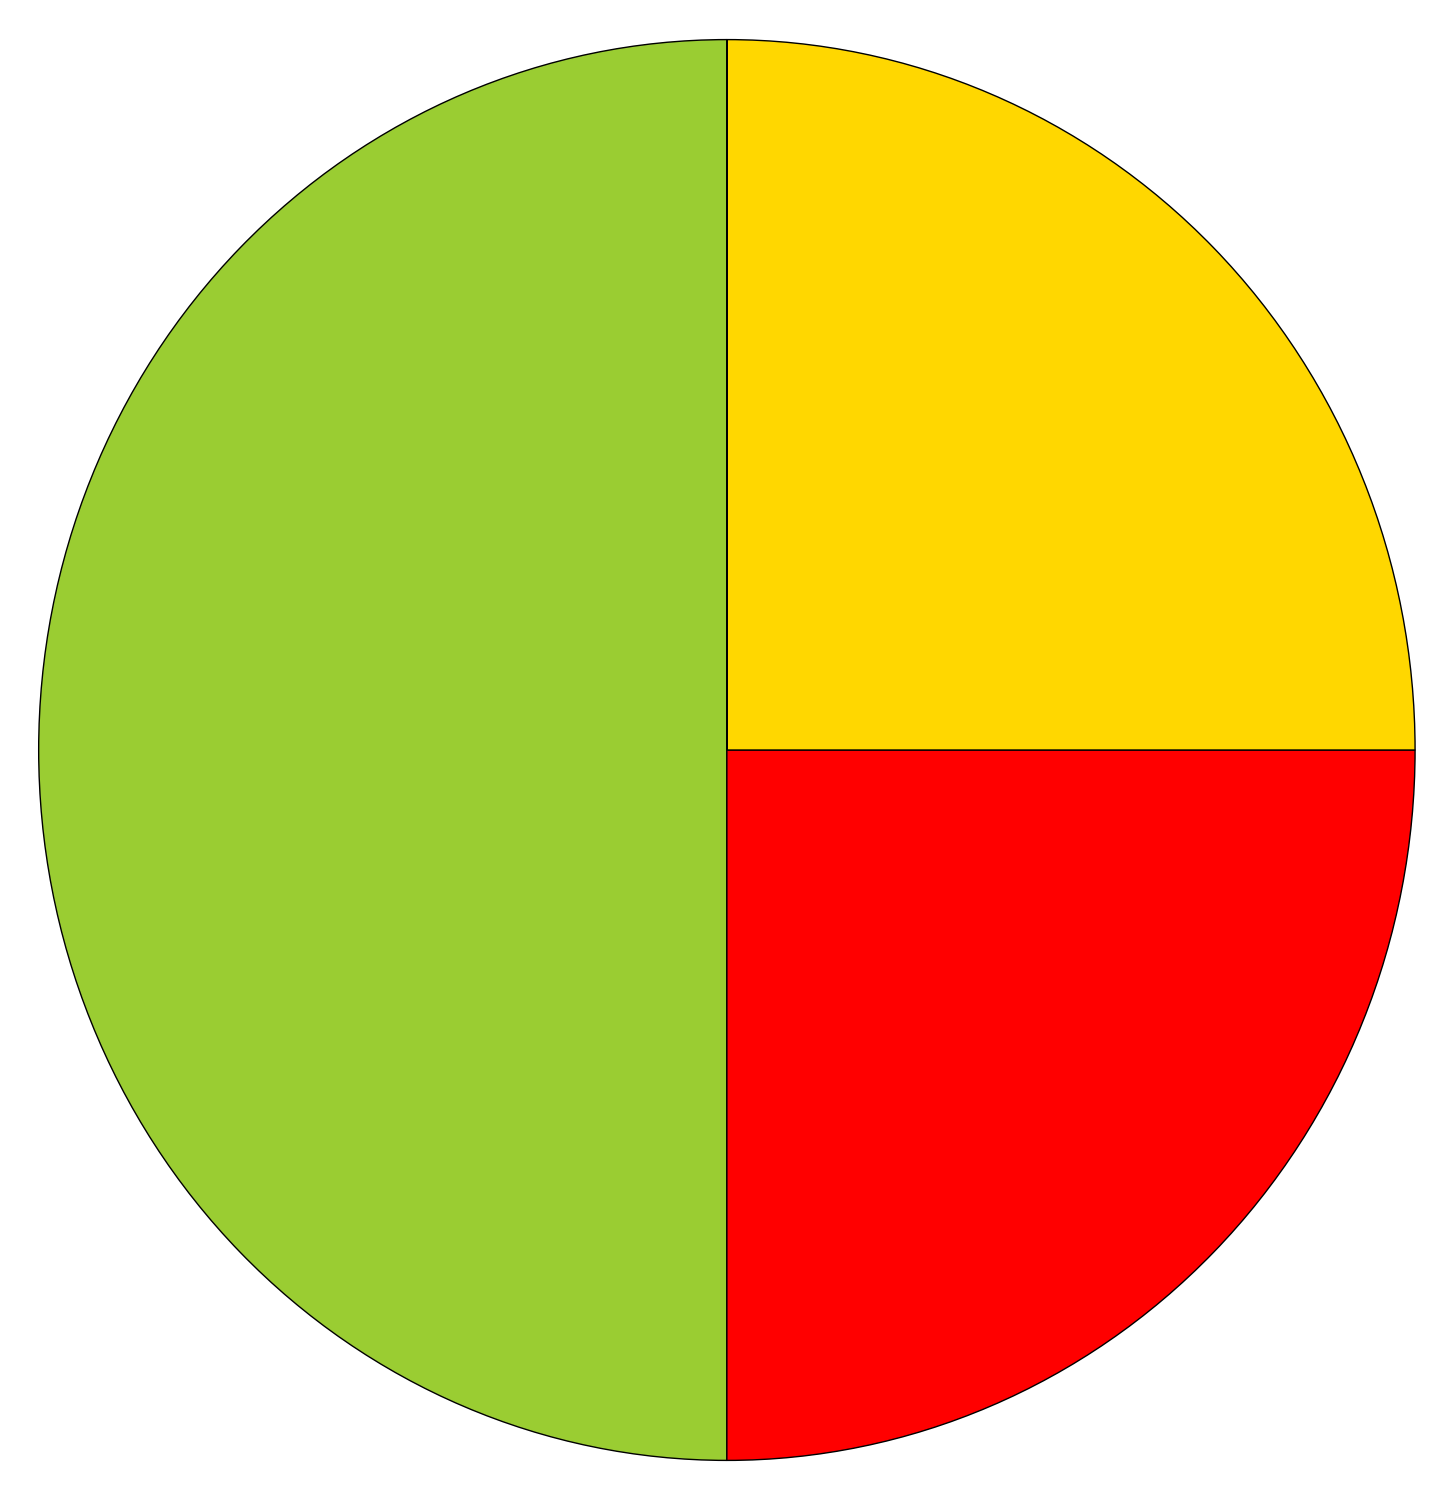
\includegraphics[width=\textwidth]{arousalALLLRgen}
    \caption{Linear regression}
  \end{subfigure}
  \hfill
  \begin{subfigure}[b]{0.3\textwidth}
    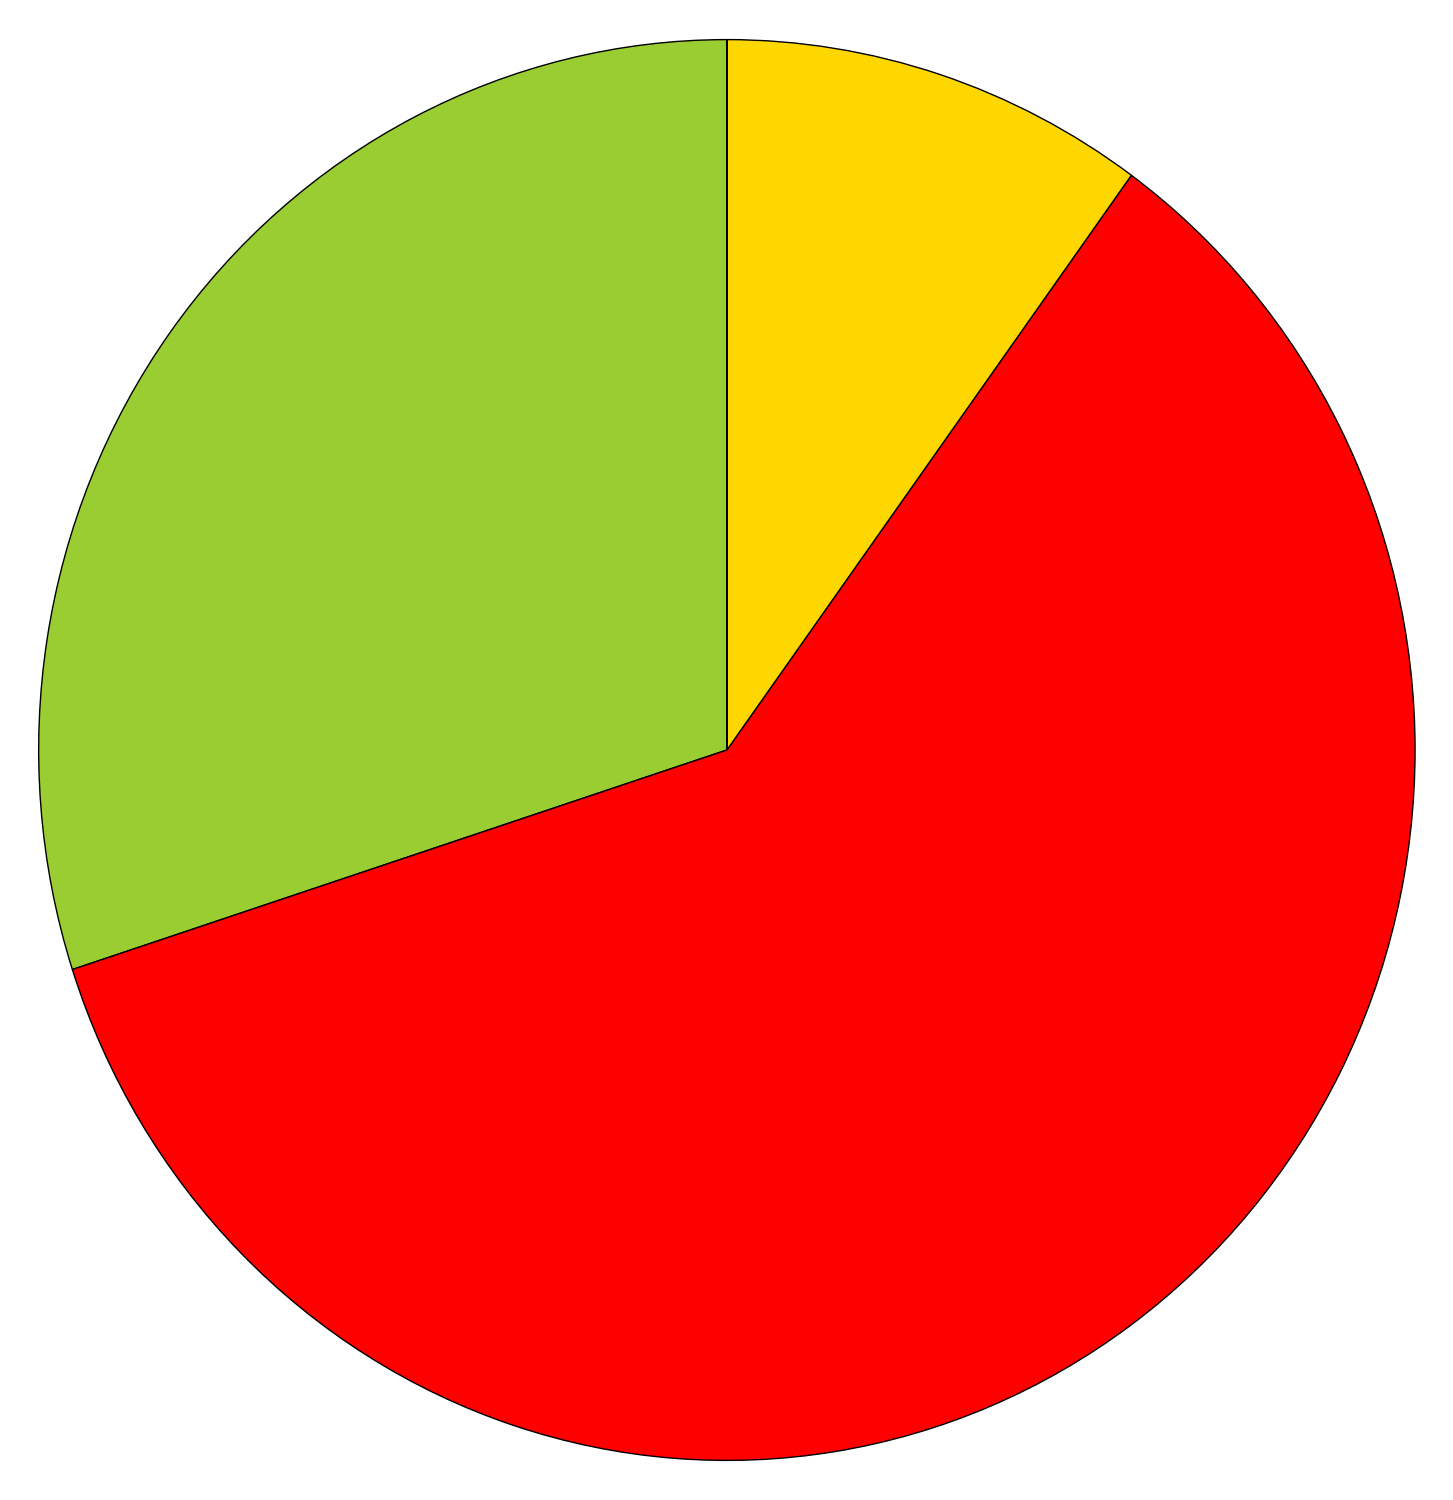
\includegraphics[width=\textwidth]{arousalALLSVMgen}
    \caption{SVM}
  \end{subfigure}
  
  \begin{subfigure}[b]{0.3\textwidth}
    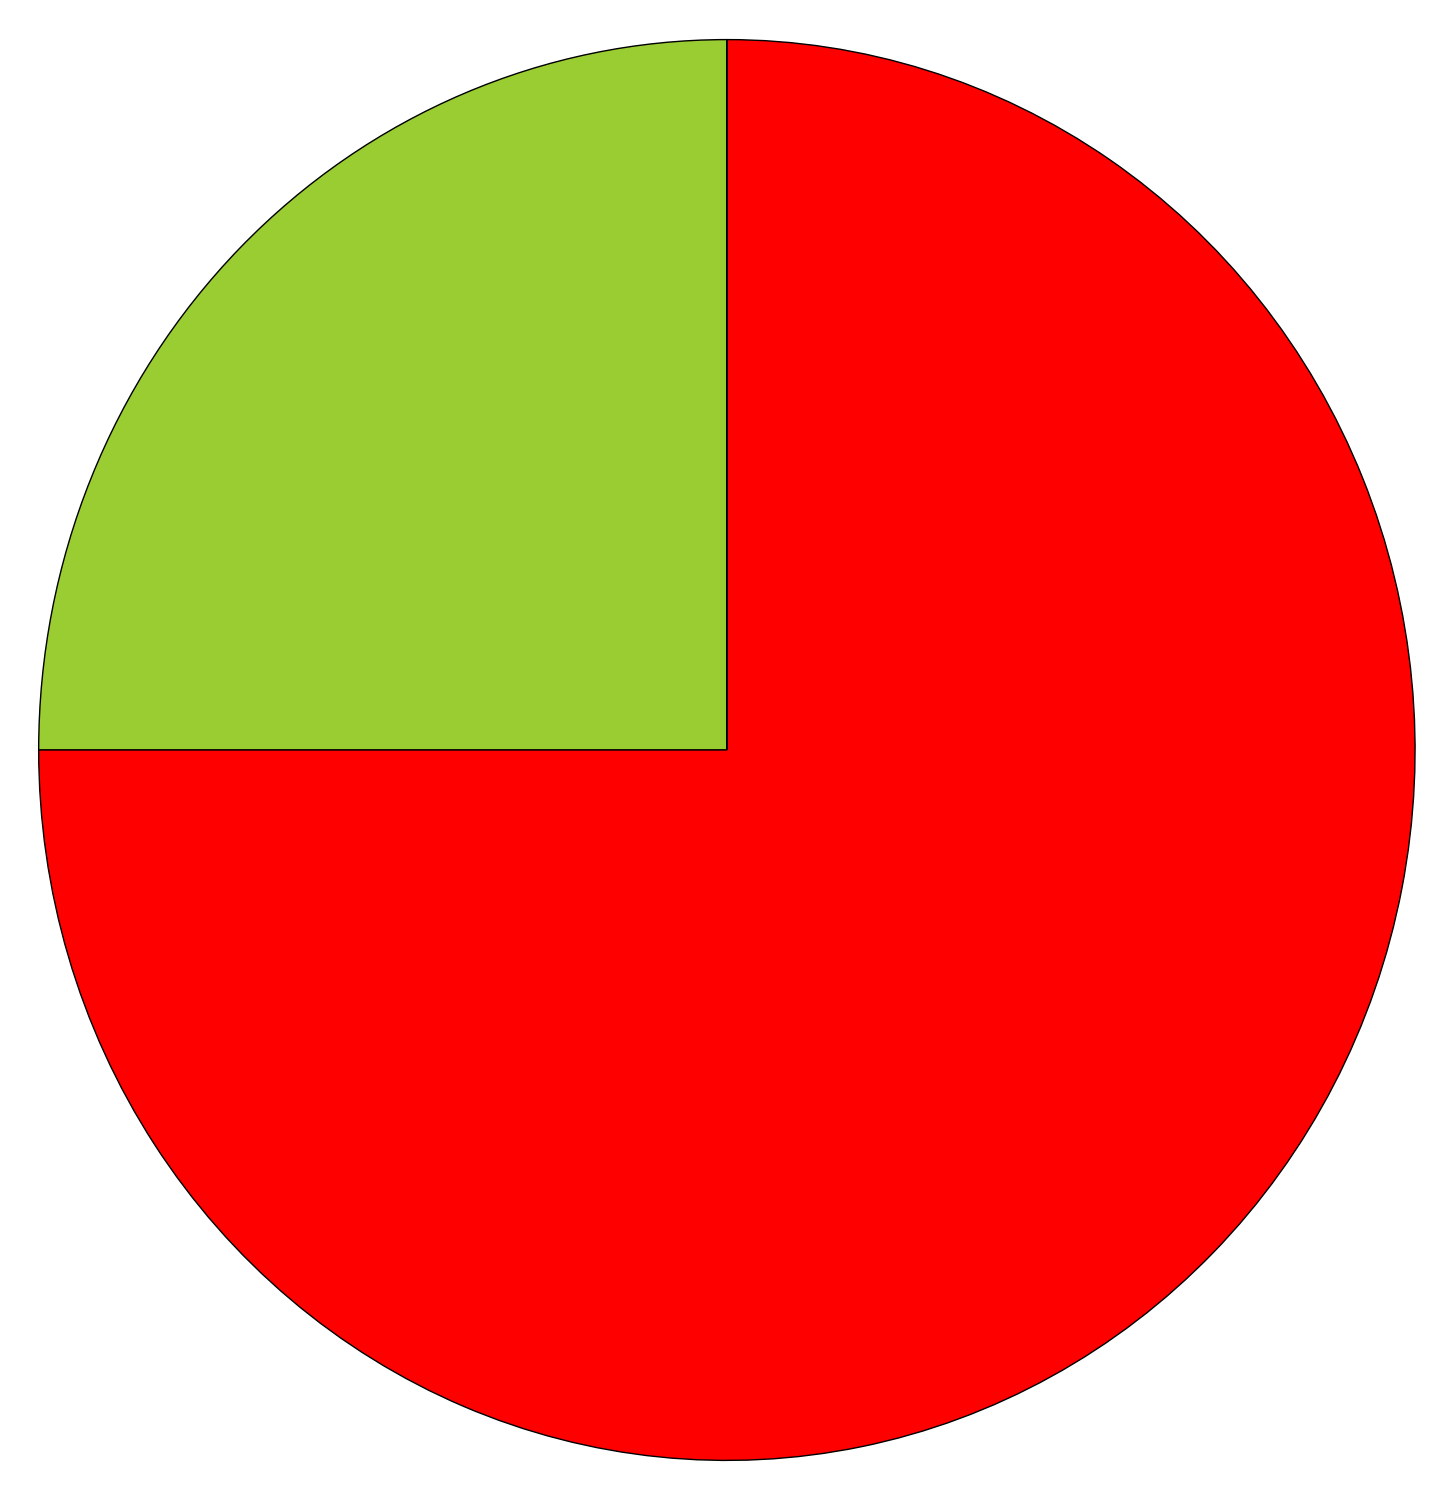
\includegraphics[width=\textwidth]{arousalALLLDAgen}
    \caption{LDA}
  \end{subfigure}
  \hfill
  \begin{subfigure}[b]{0.3\textwidth}
    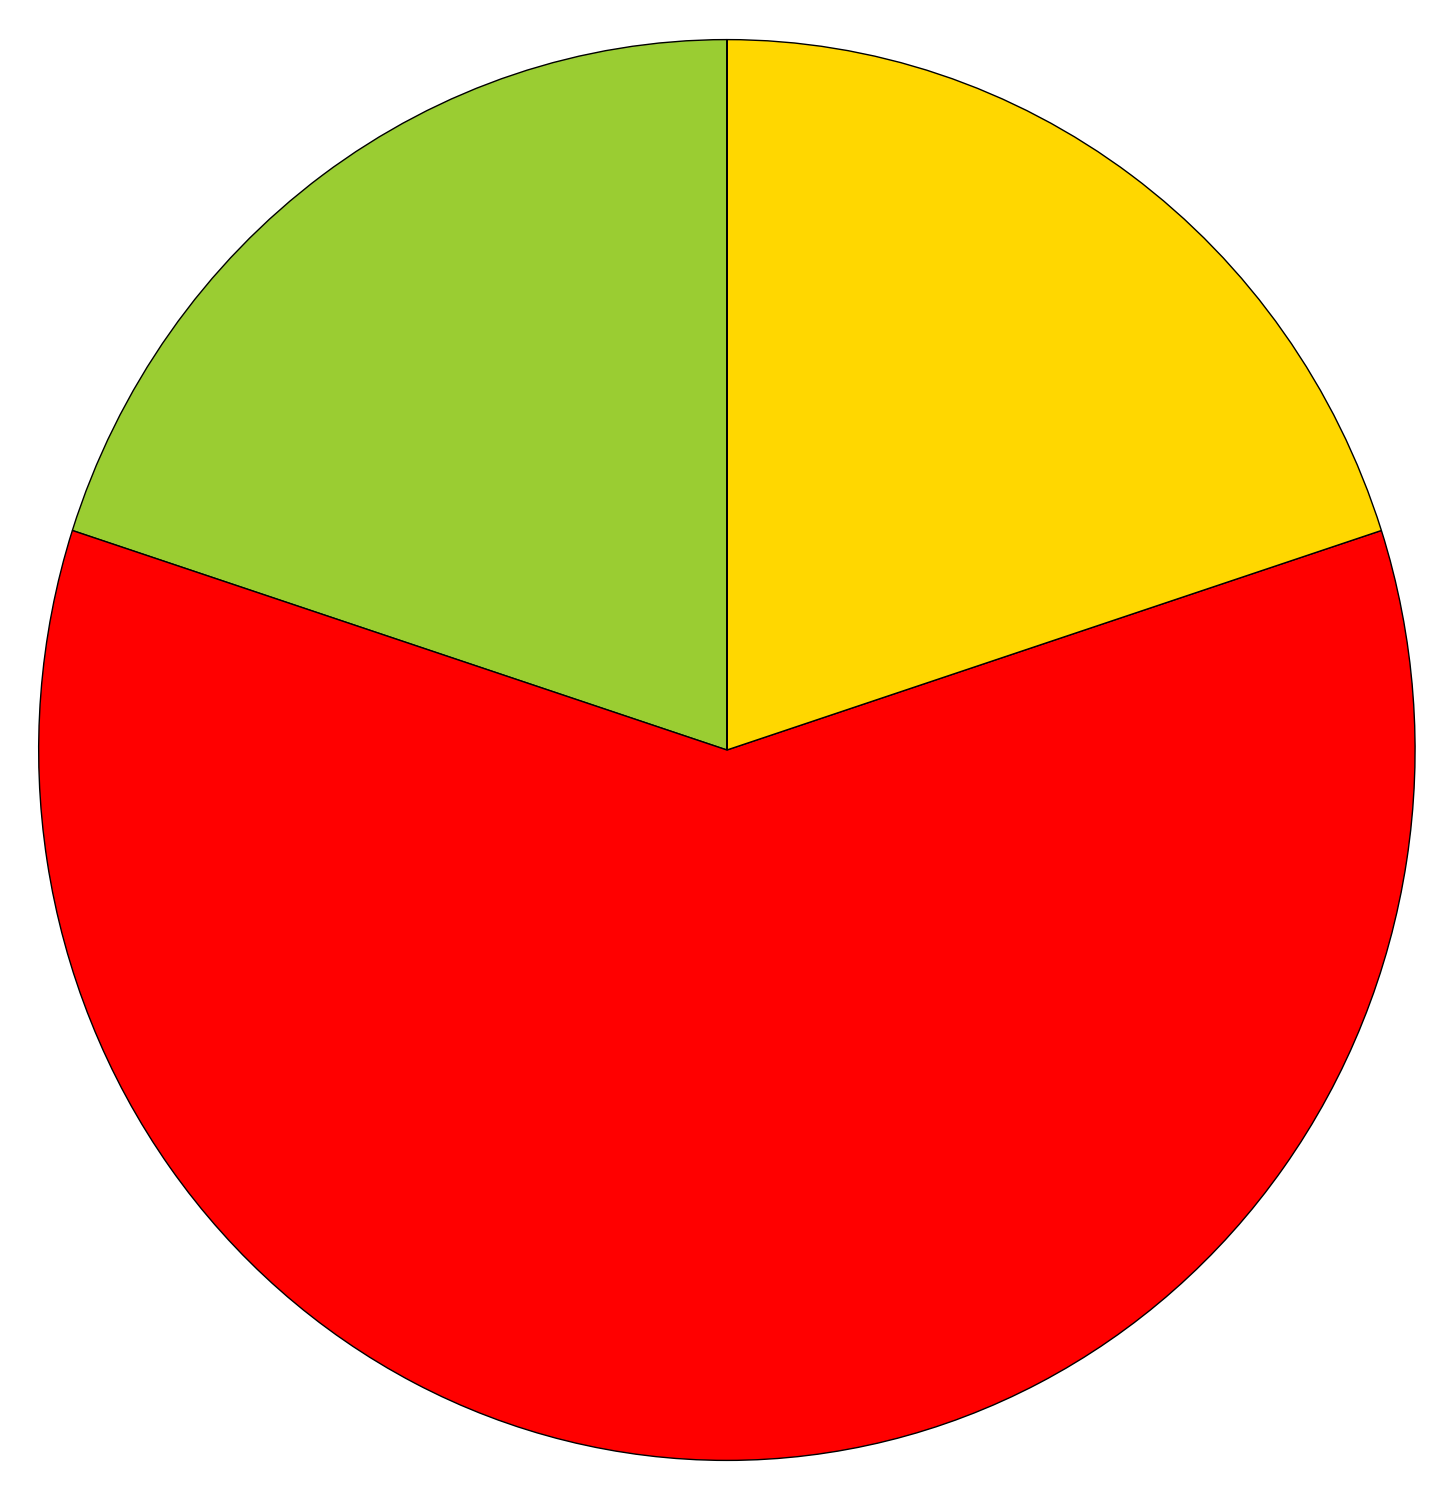
\includegraphics[width=\textwidth]{arousalALLL1gen}
    \caption{Lasso regression}
  \end{subfigure}
  \hfill
  \begin{subfigure}[b]{0.3\textwidth}
    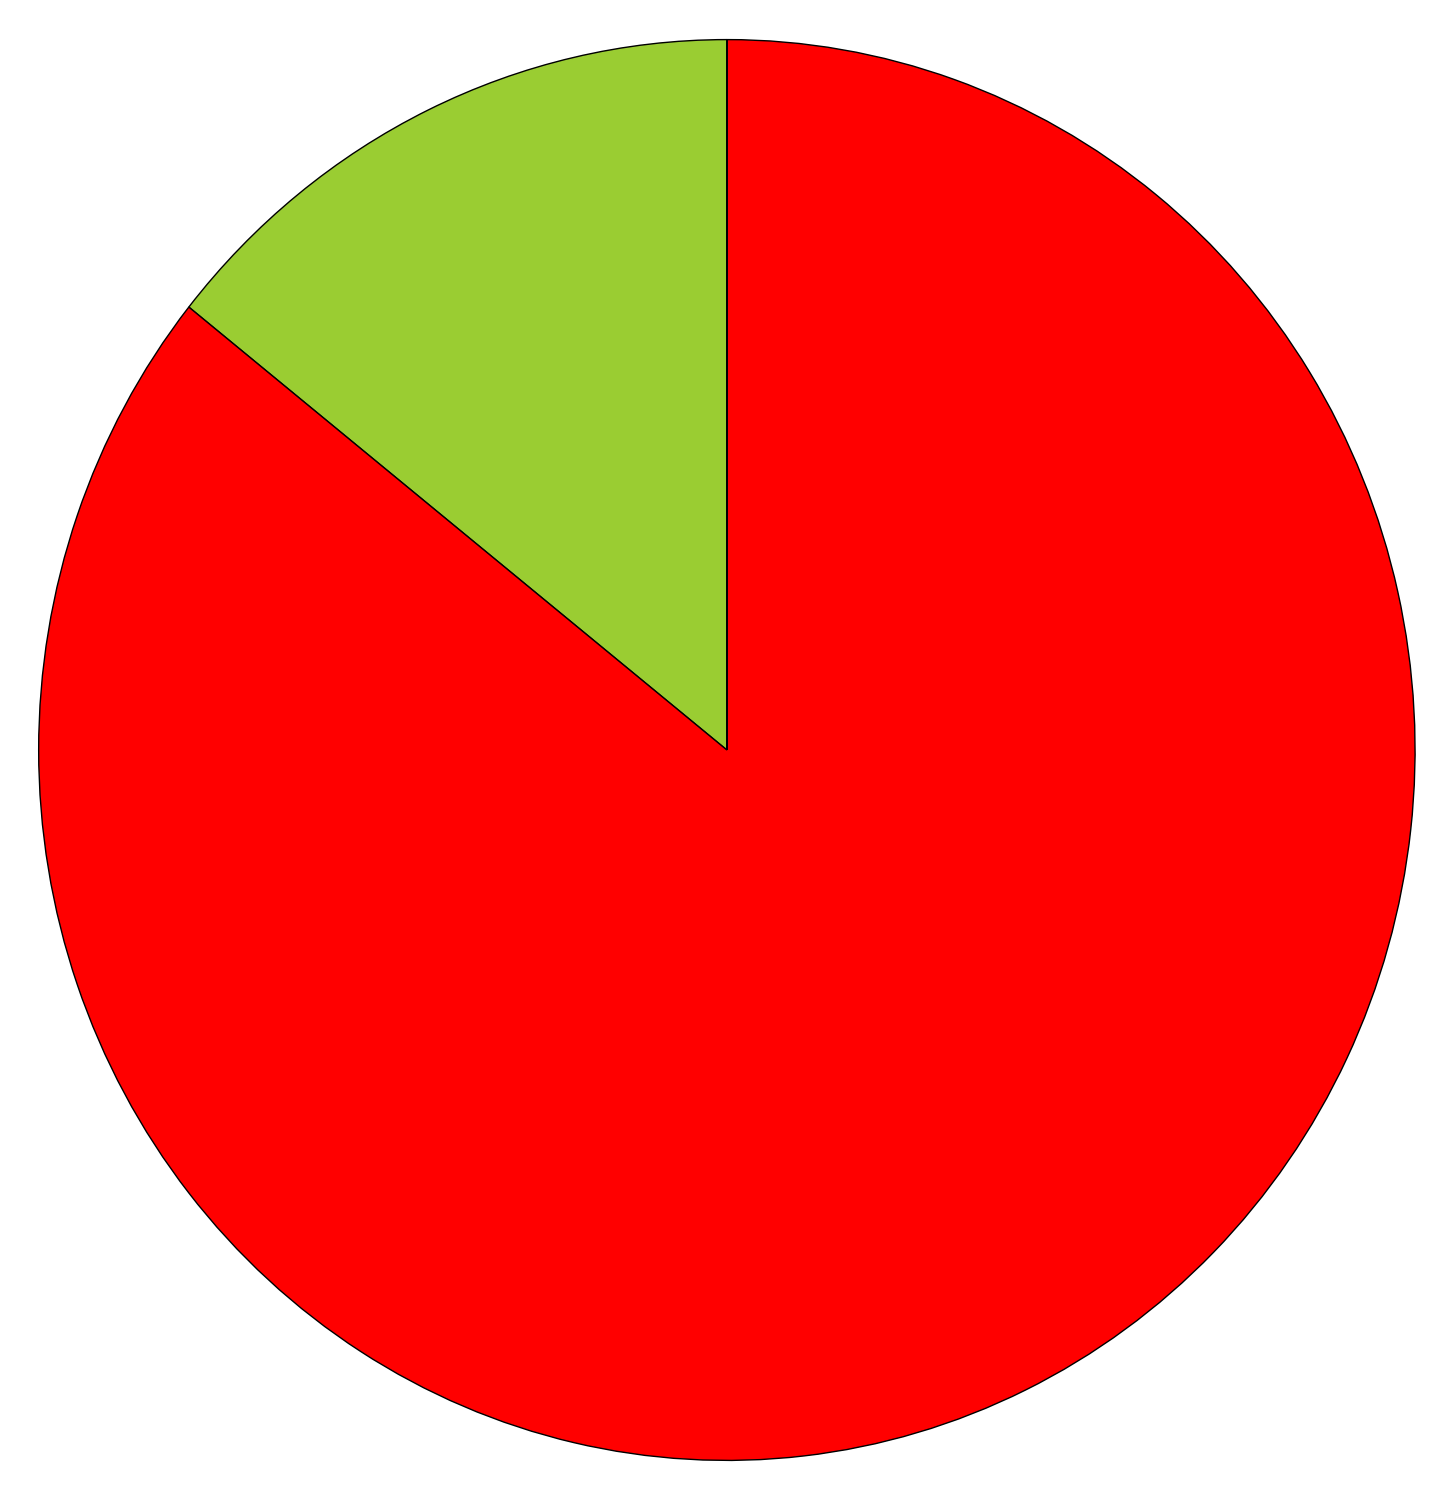
\includegraphics[width=\textwidth]{arousalALLL2gen}
    \caption{Ridge regression}
  \end{subfigure}
  
  \begin{subfigure}[b]{0.3\textwidth}
    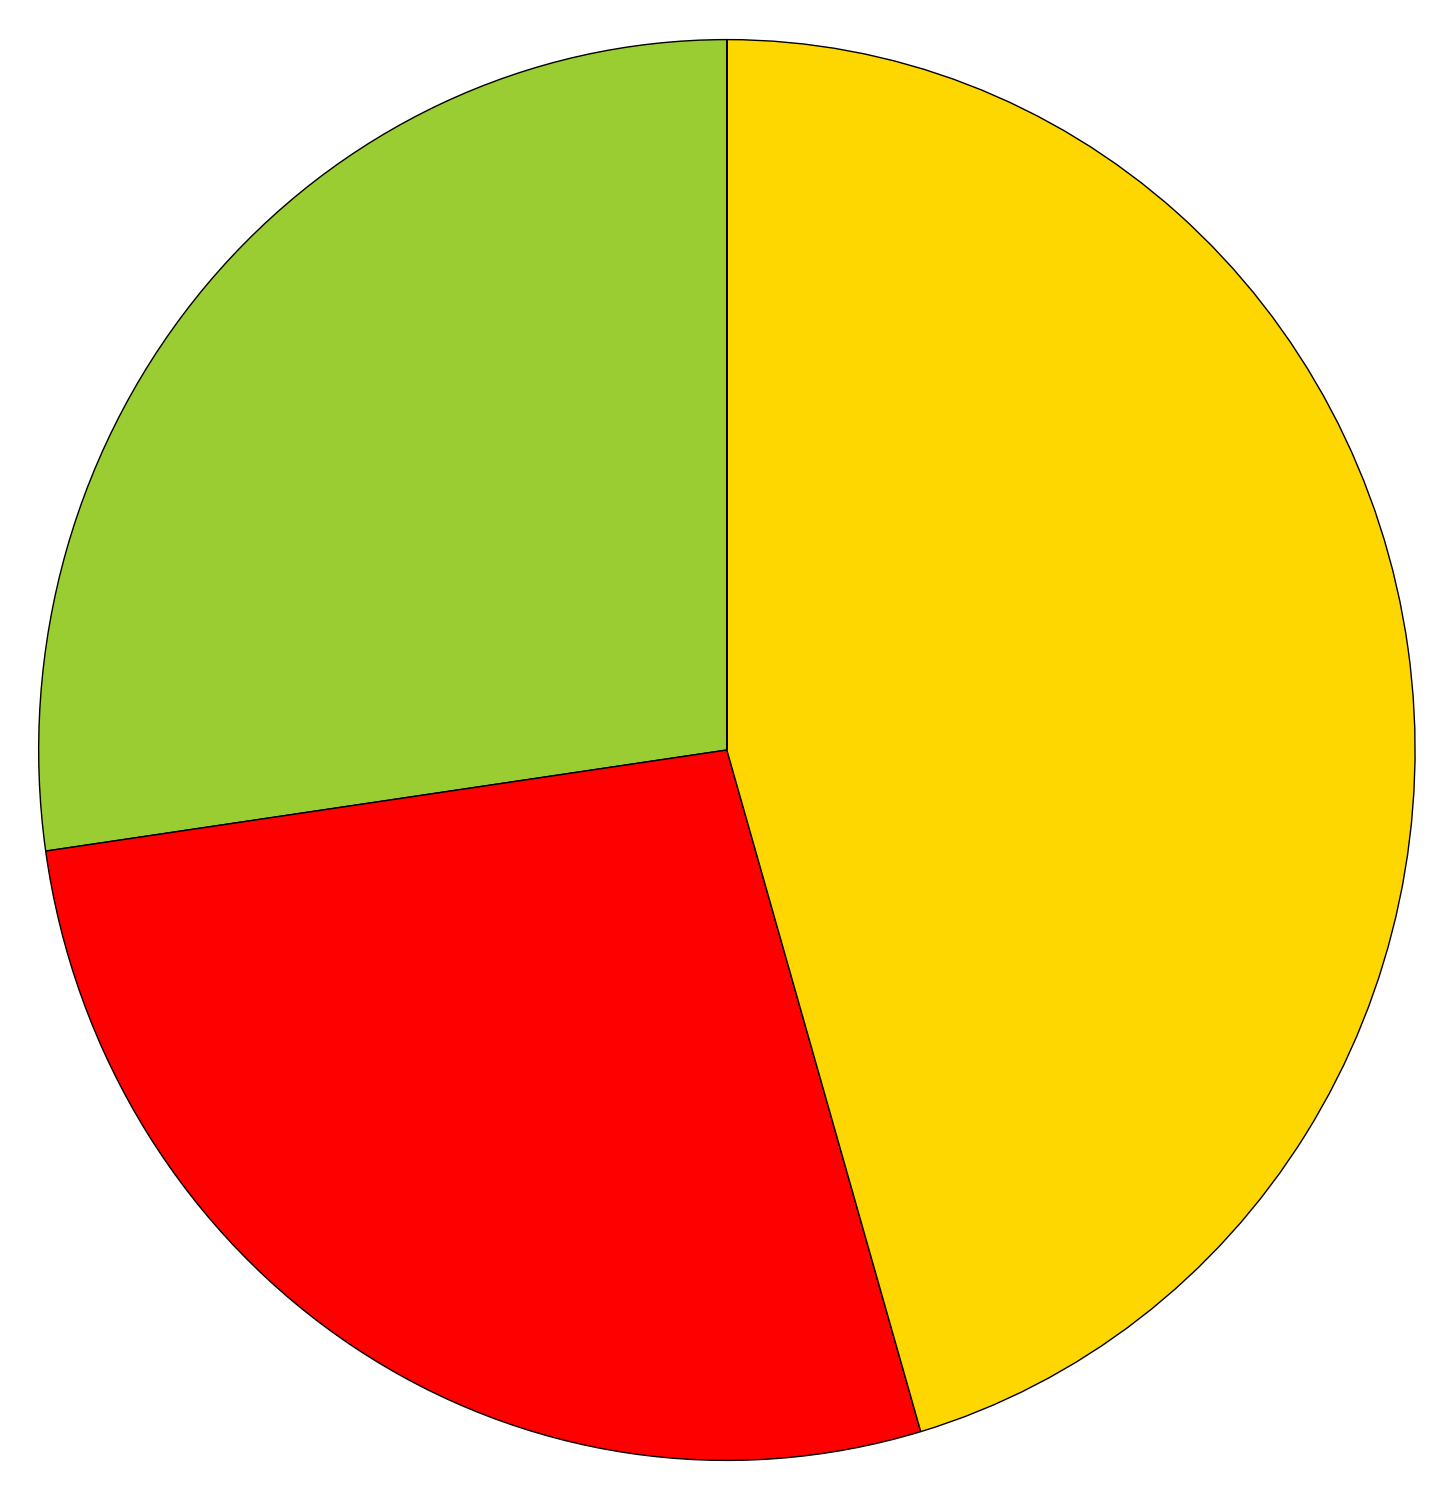
\includegraphics[width=\textwidth]{arousalALLRFgen}
    \caption{Random forests}
  \end{subfigure}
  \hfill
  \begin{subfigure}[b]{0.3\textwidth}
    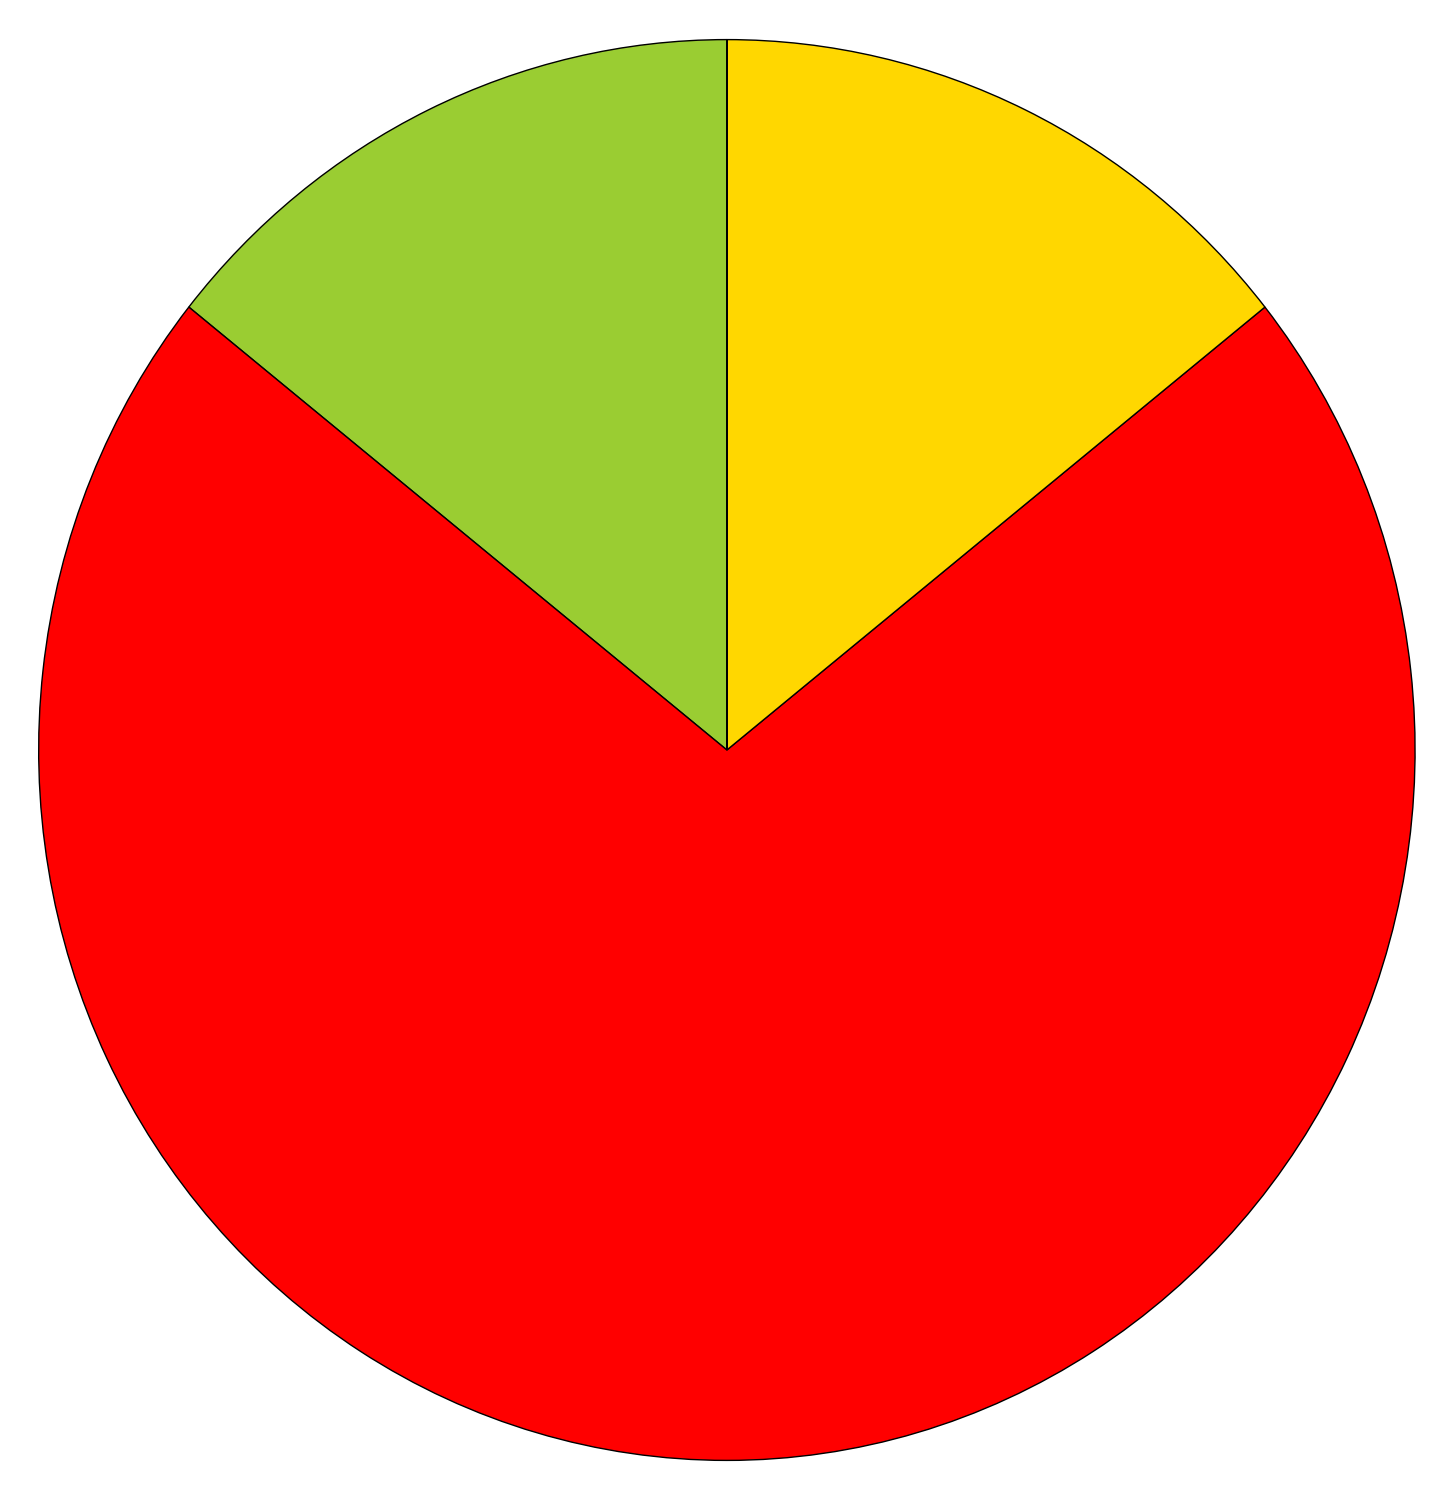
\includegraphics[width=\textwidth]{arousalALLPCAgen}
    \caption{PCA}
  \end{subfigure}
  \hfill
  \begin{subfigure}[b]{0.3\textwidth}
    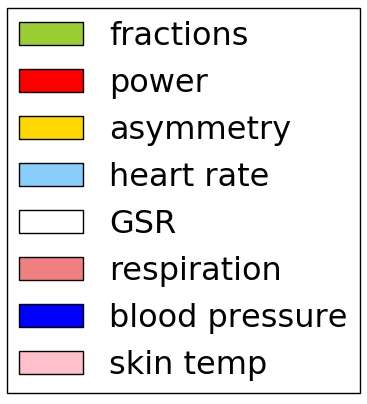
\includegraphics[width=\textwidth]{legend}
    \caption{Legend\label{arousalpieslegendgen}}
  \end{subfigure}
\end{figure}

\clearpage

\begin{figure}[!tbp]
  \centering
  \caption{Selection features for valence classification.\label{valencepiesgen}}
  \begin{subfigure}[b]{0.3\textwidth}
    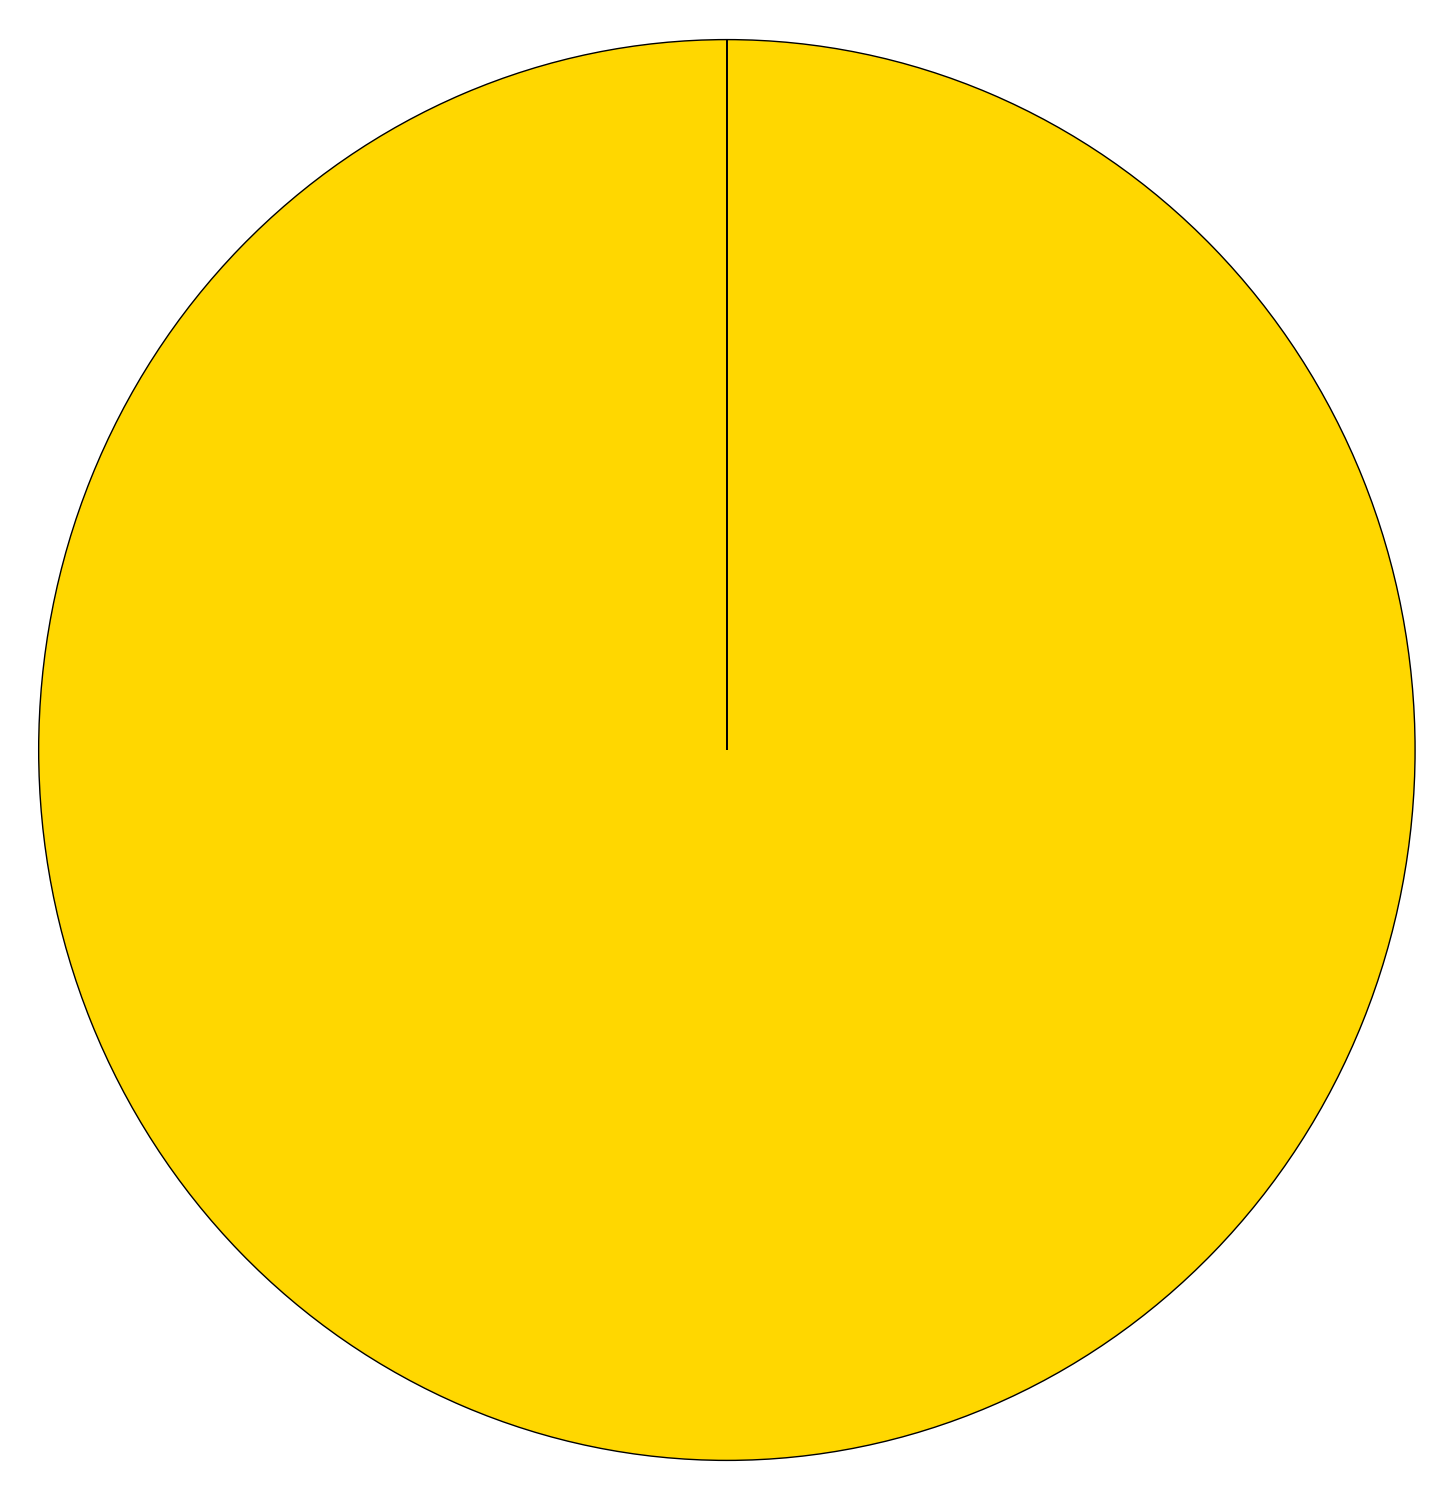
\includegraphics[width=\textwidth]{valenceALLpearsonRgen}
    \caption{Pearson correlation}
  \end{subfigure}
  \hfill
  \begin{subfigure}[b]{0.3\textwidth}
    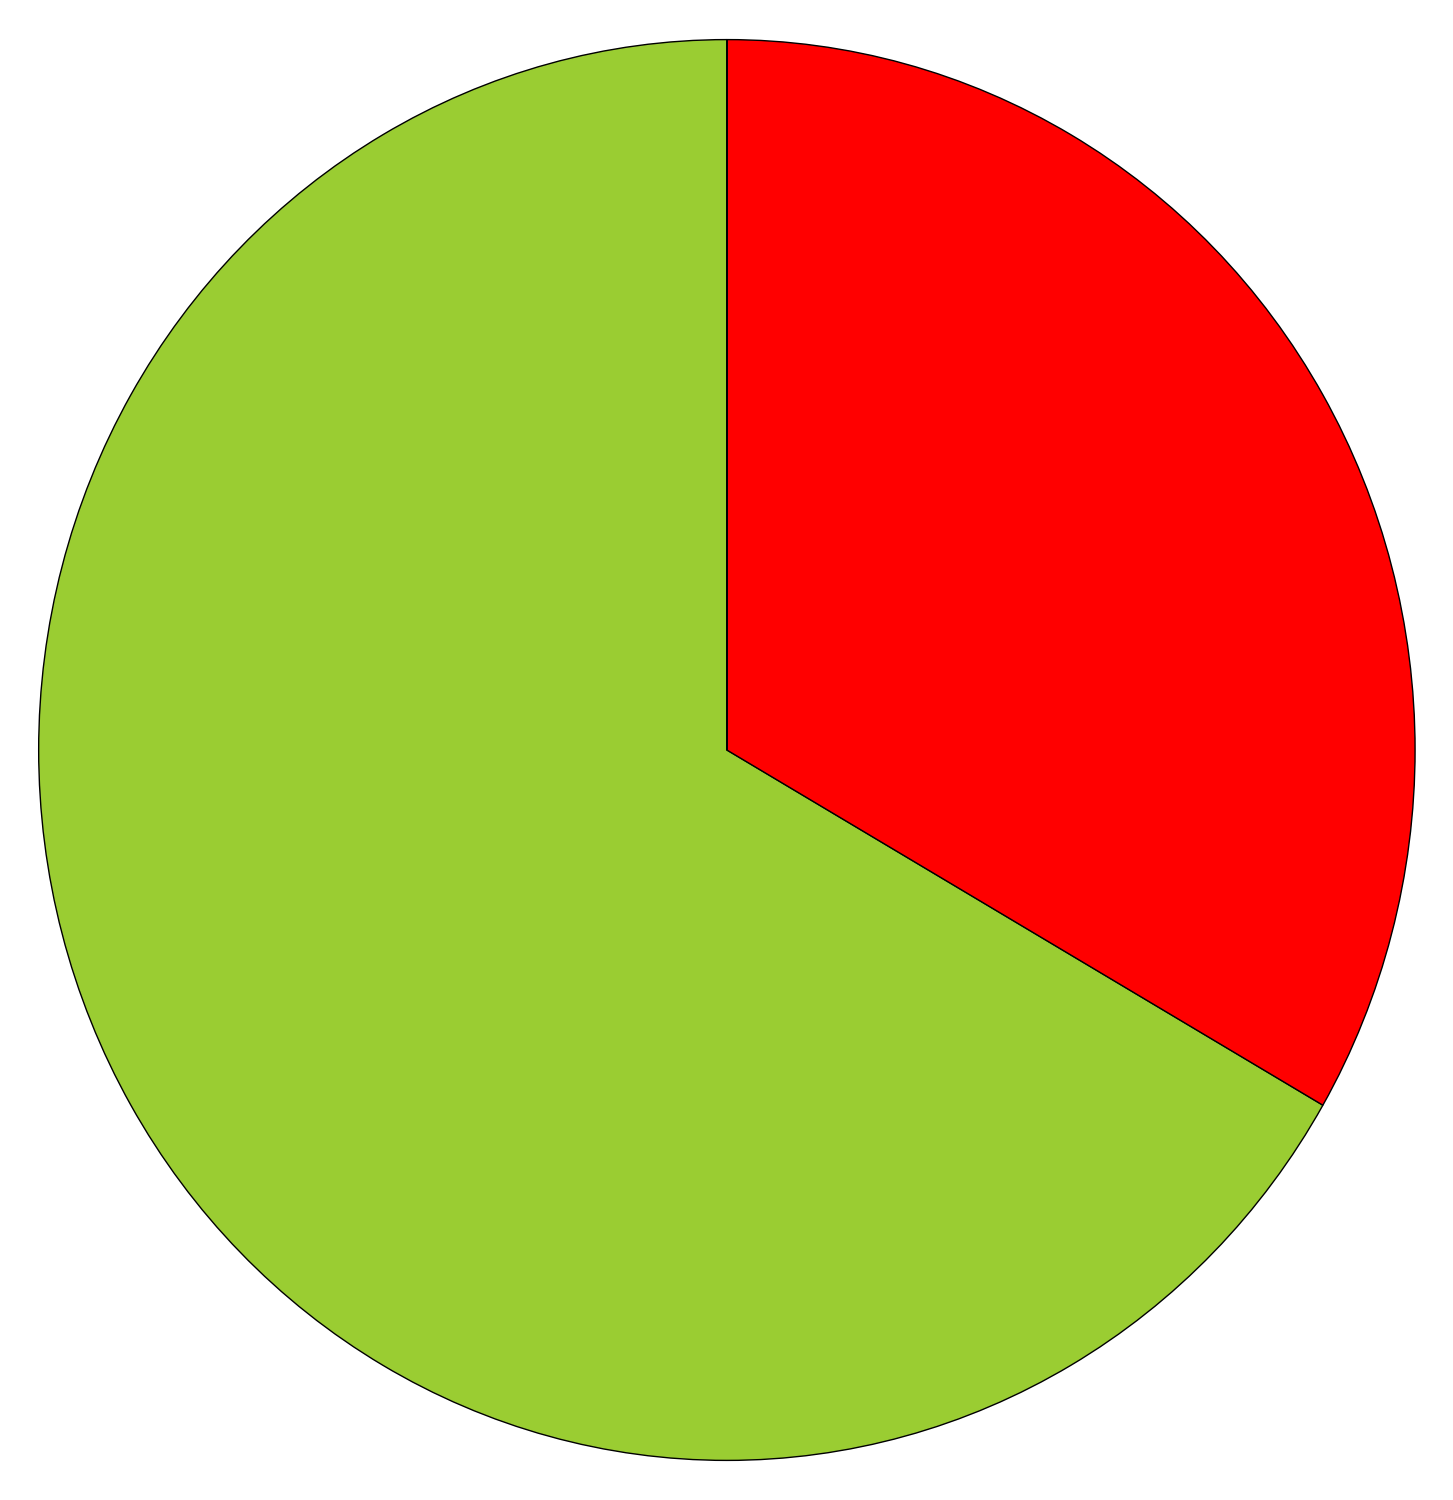
\includegraphics[width=\textwidth]{valenceALLMutInfgen}
    \caption{Mutual information}
  \end{subfigure}
  \hfill
  \begin{subfigure}[b]{0.3\textwidth}
    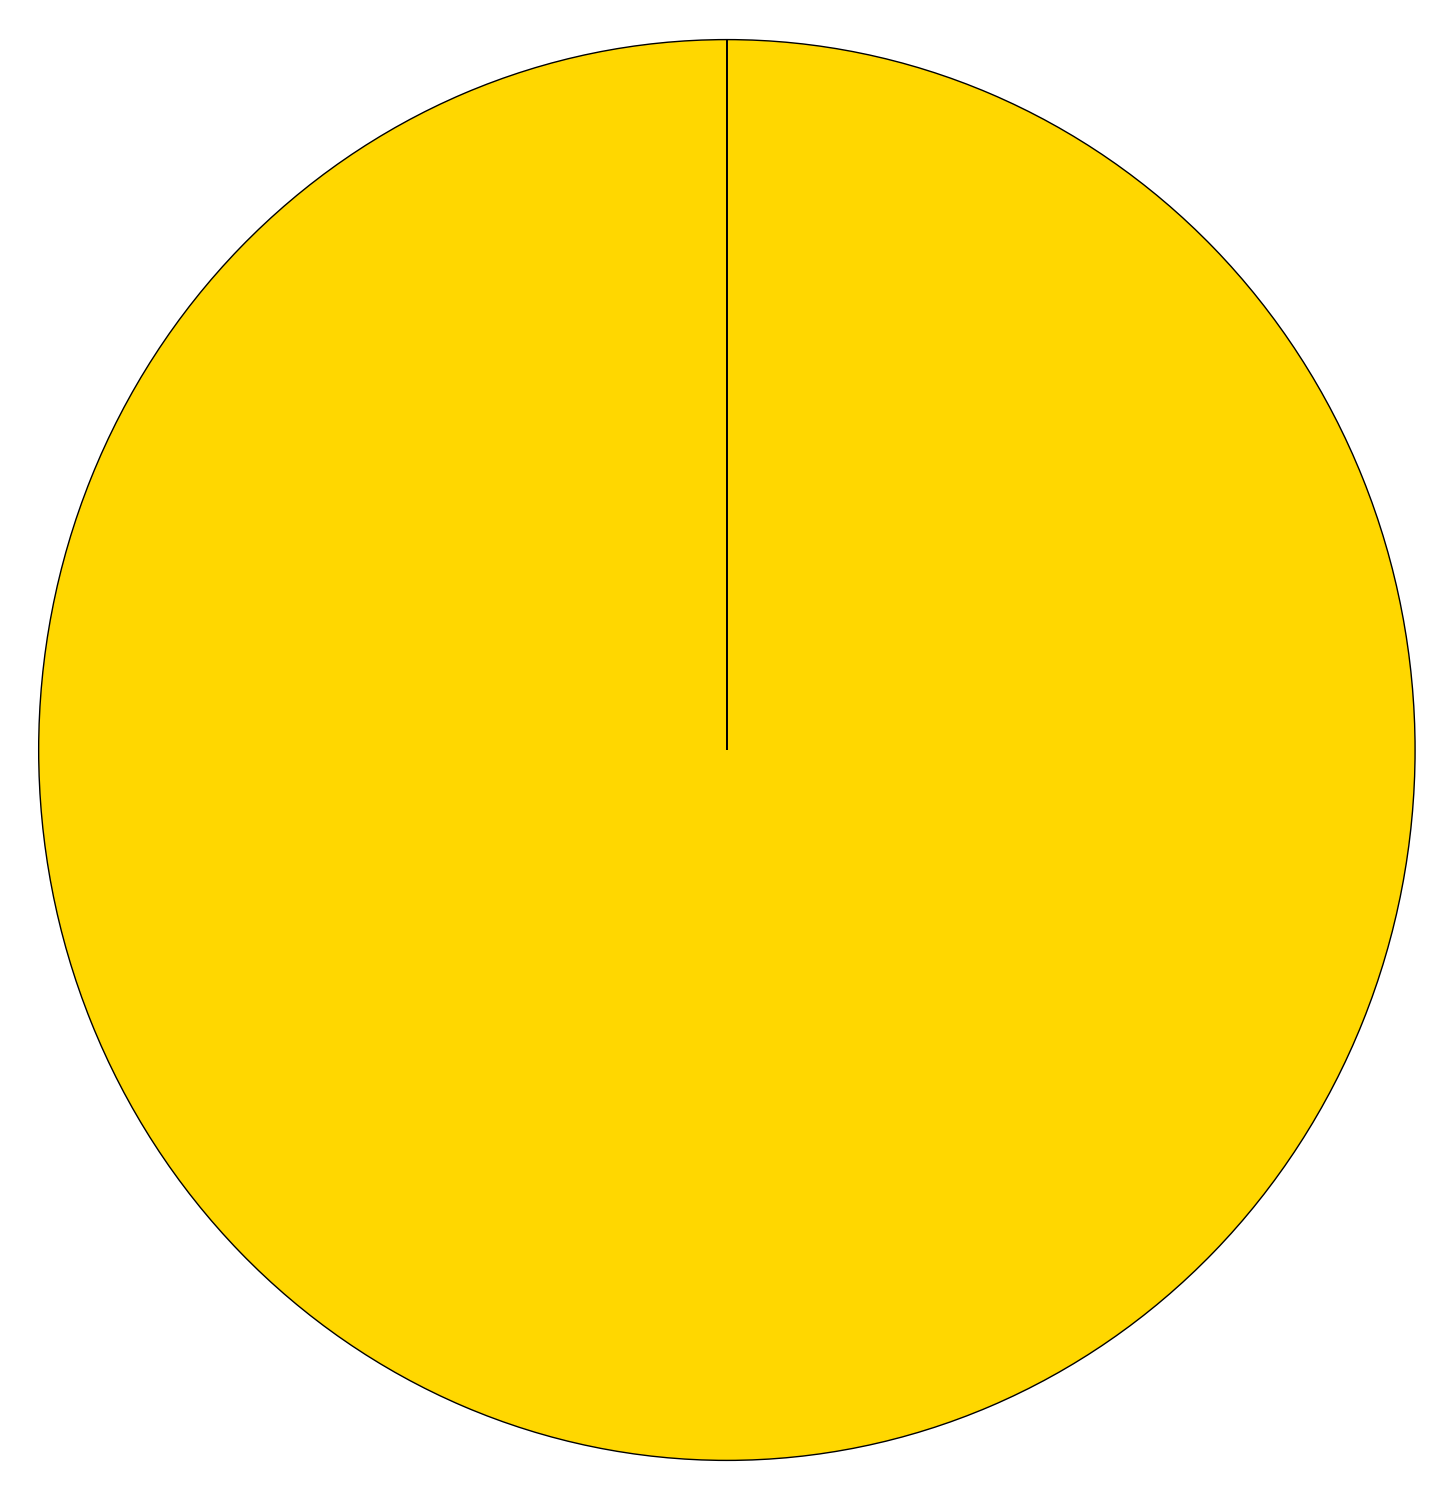
\includegraphics[width=\textwidth]{valenceALLdCorrgen}
    \caption{Distance Correlation}
  \end{subfigure}
  
  \begin{subfigure}[b]{0.3\textwidth}
    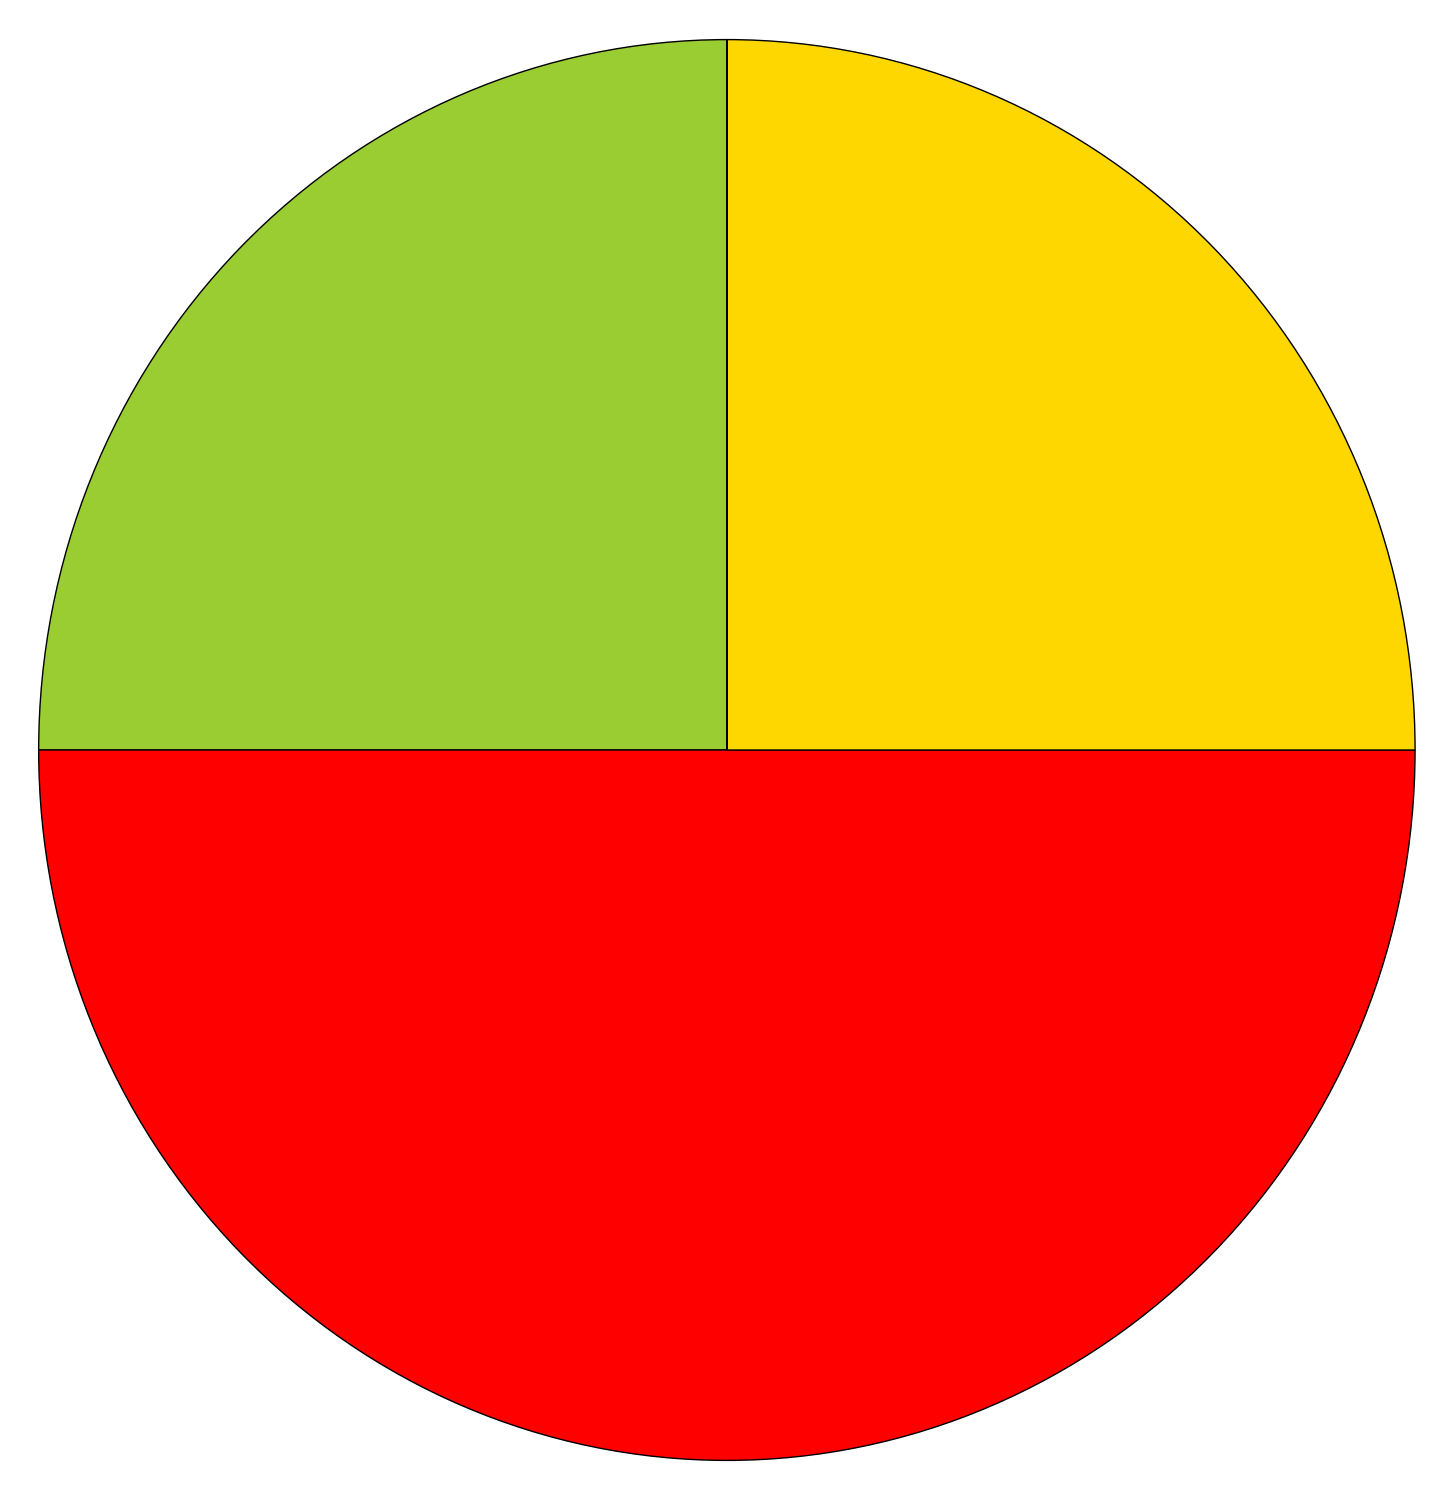
\includegraphics[width=\textwidth]{valenceALLANOVAgen}
    \caption{ANOVA}
  \end{subfigure}
  \hfill
  \begin{subfigure}[b]{0.3\textwidth}
    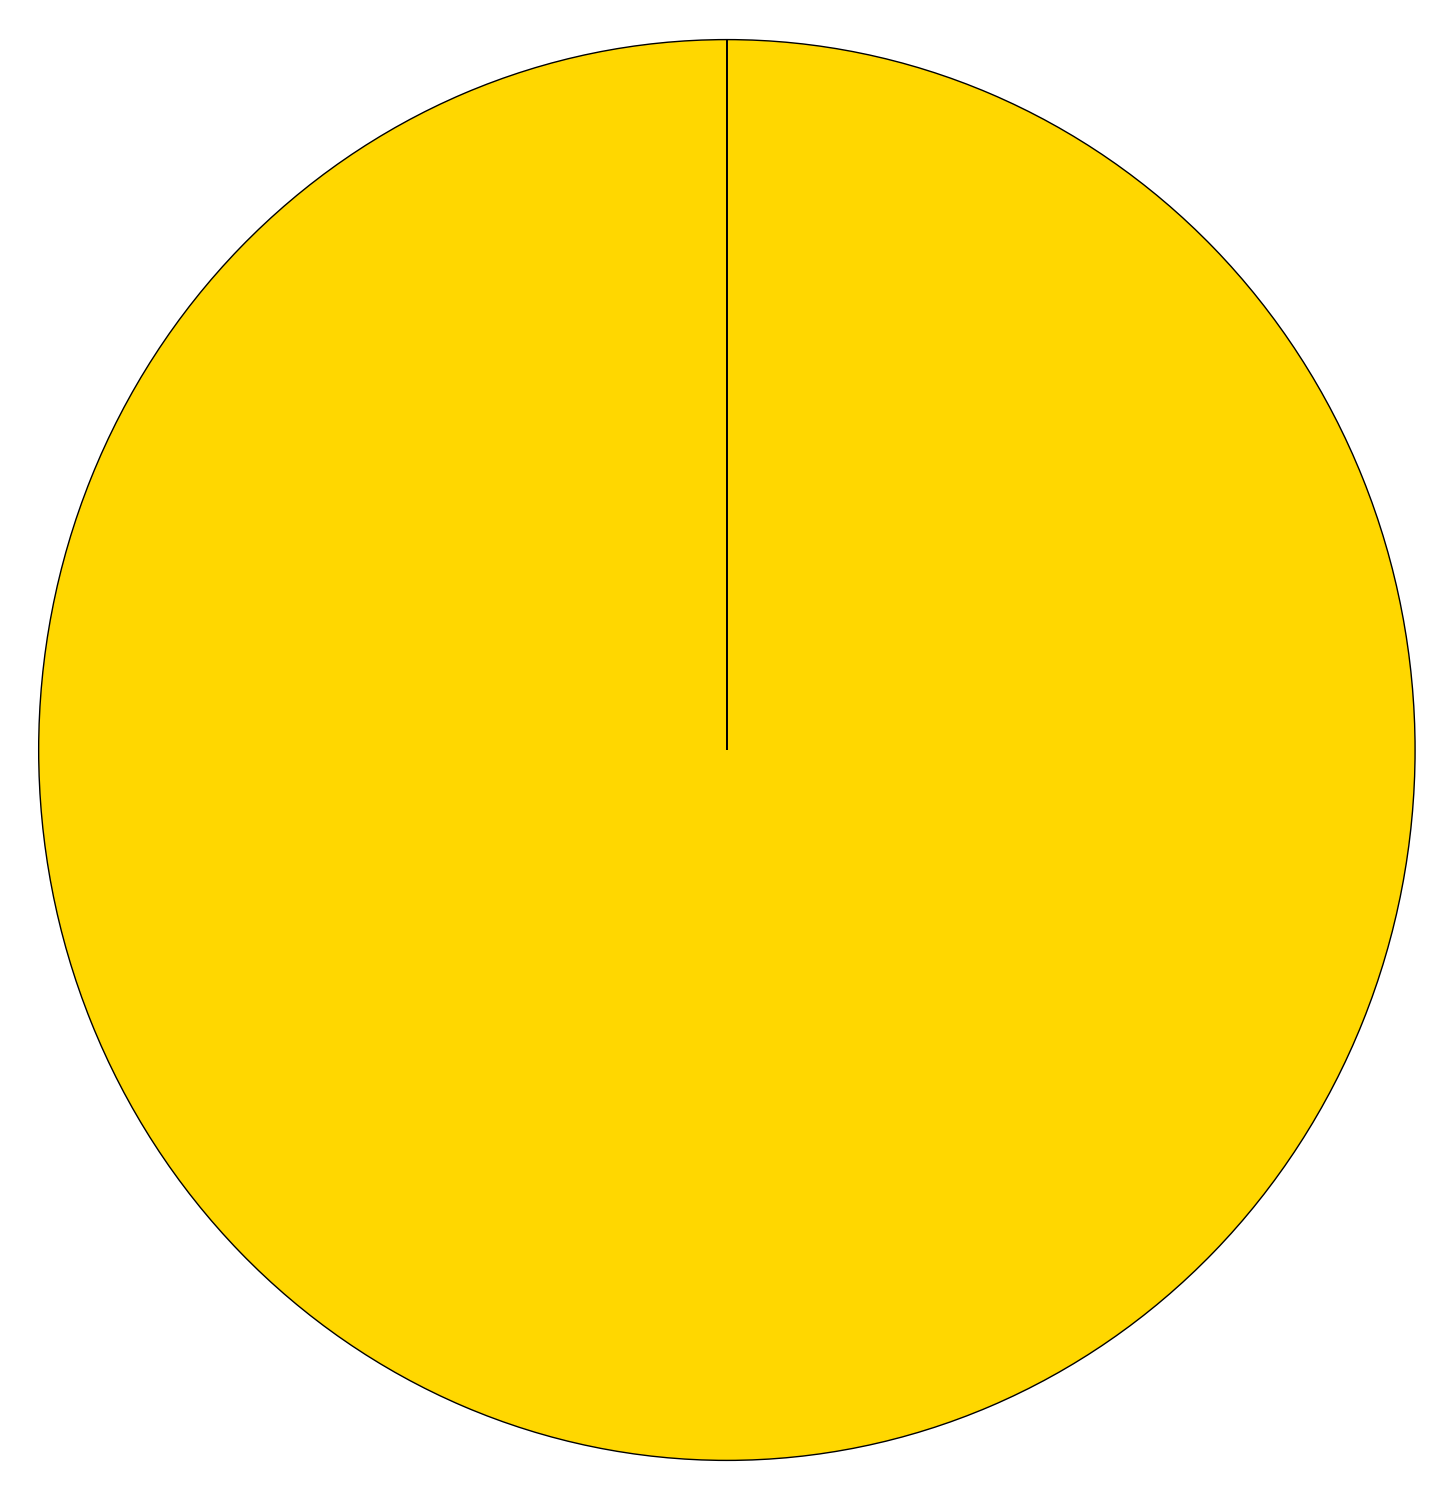
\includegraphics[width=\textwidth]{valenceALLLRgen}
    \caption{Linear regression}
  \end{subfigure}
  \hfill
  \begin{subfigure}[b]{0.3\textwidth}
    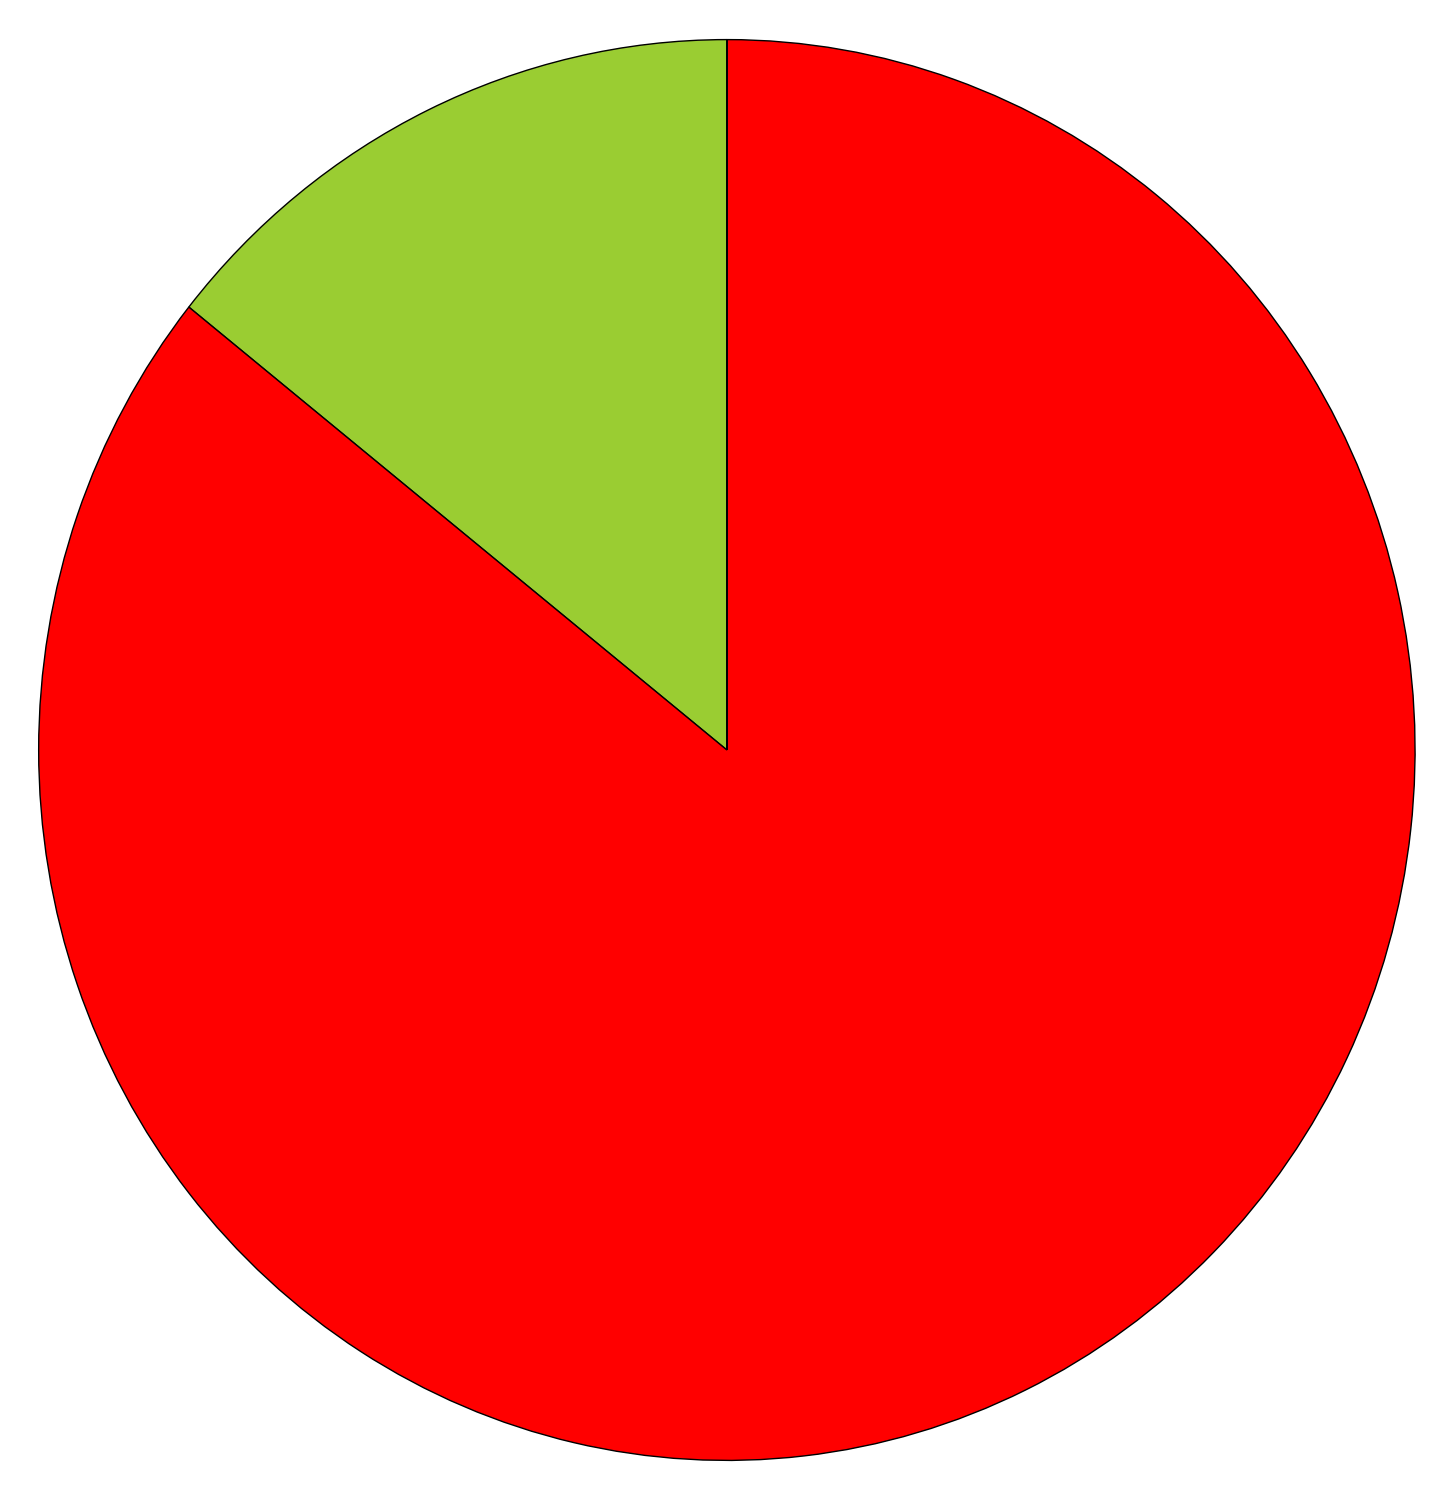
\includegraphics[width=\textwidth]{valenceALLSVMgen}
    \caption{SVM}
  \end{subfigure}
  
  \begin{subfigure}[b]{0.3\textwidth}
    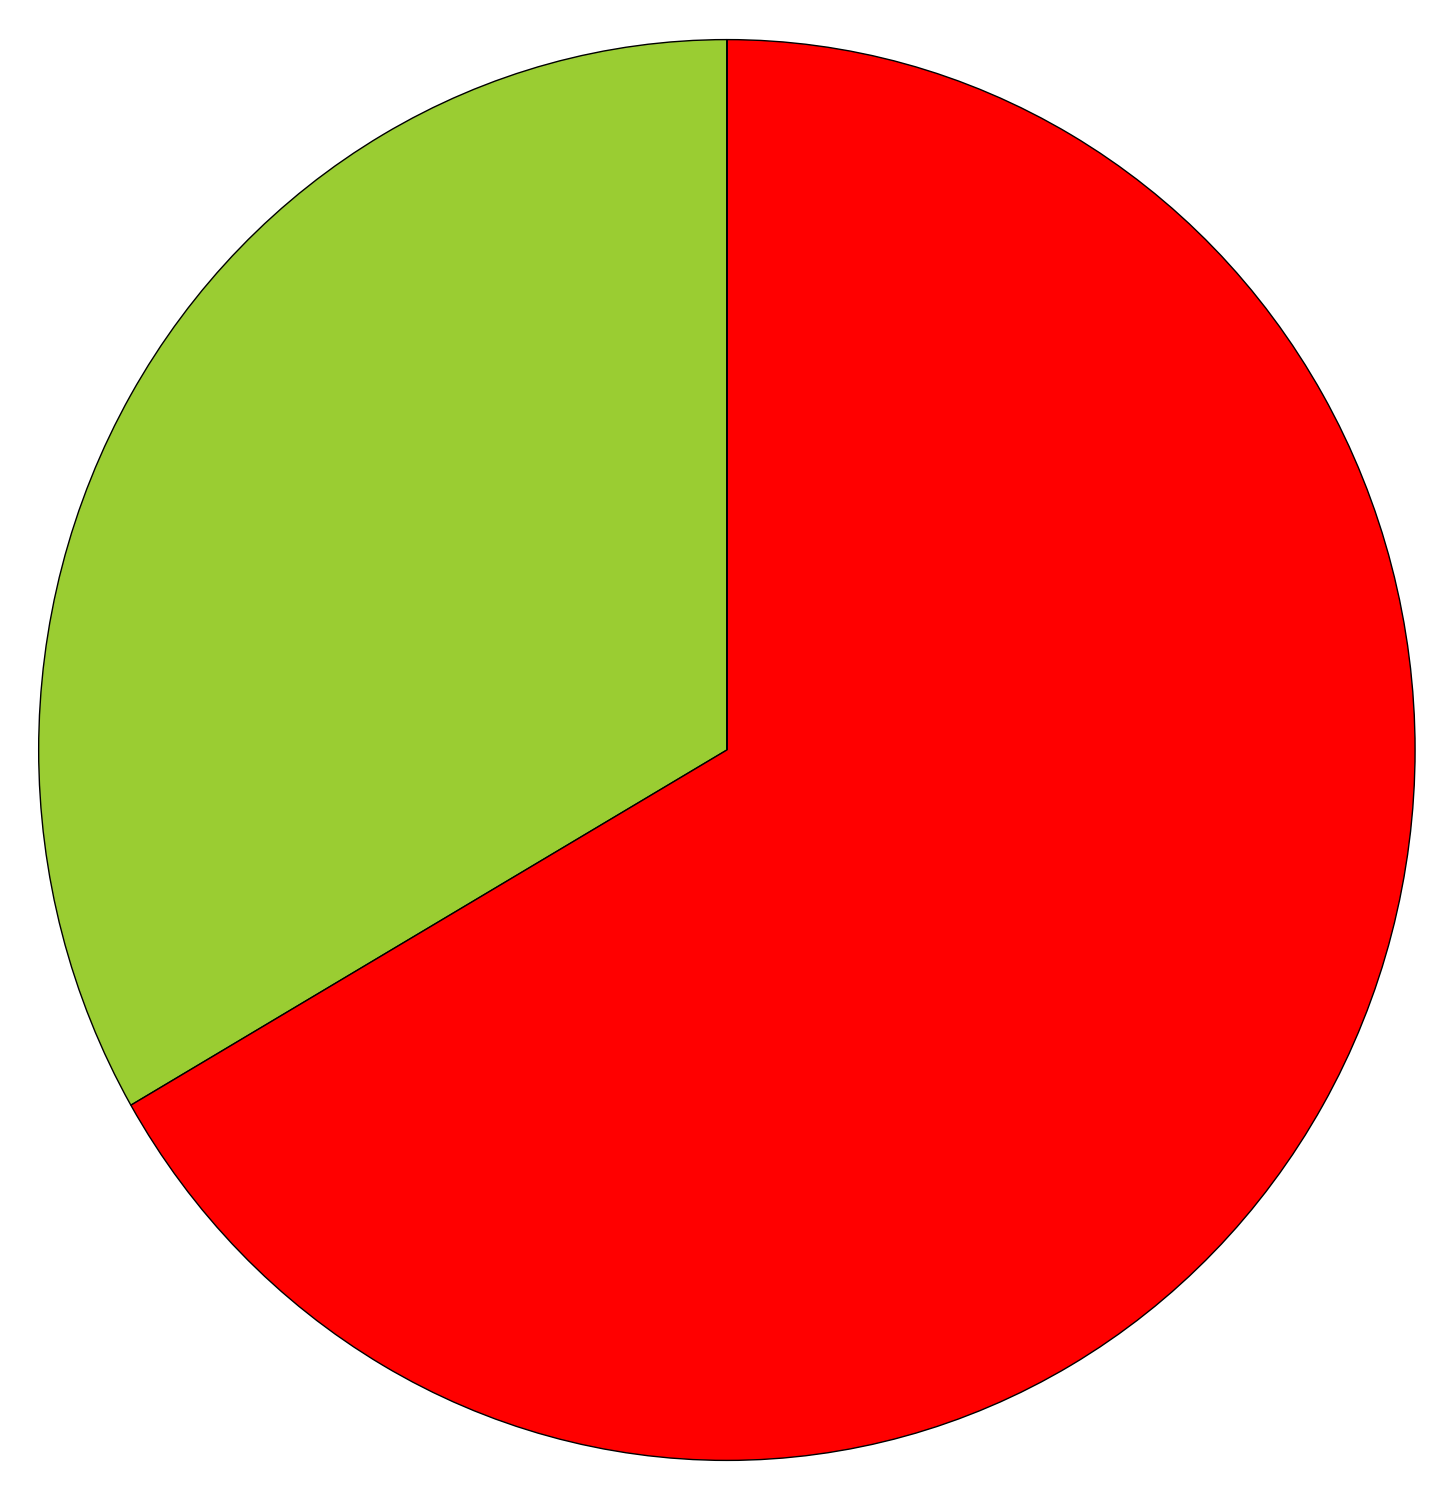
\includegraphics[width=\textwidth]{valenceALLLDAgen}
    \caption{LDA}
  \end{subfigure}
  \hfill
  \begin{subfigure}[b]{0.3\textwidth}
    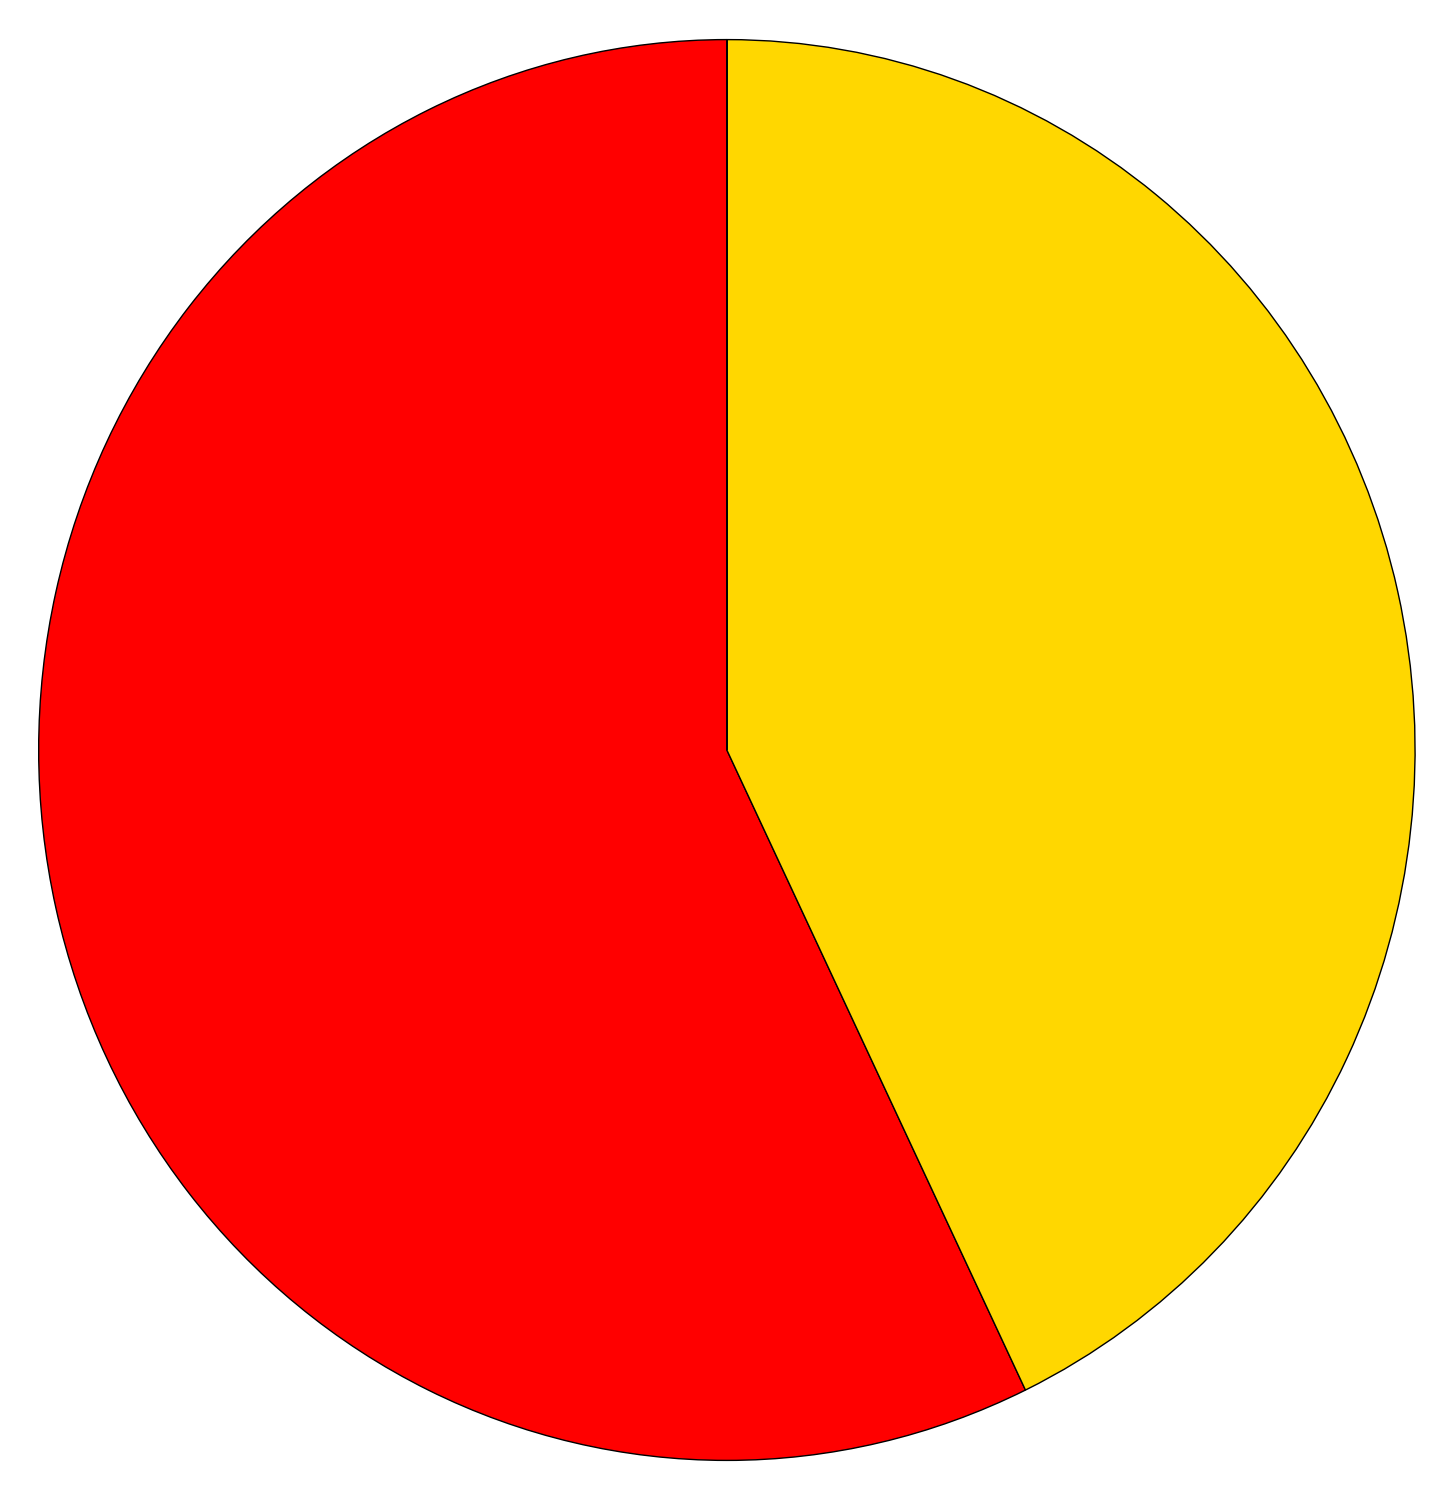
\includegraphics[width=\textwidth]{valenceALLL1gen}
    \caption{Lasso regression}
  \end{subfigure}
  \hfill
  \begin{subfigure}[b]{0.3\textwidth}
    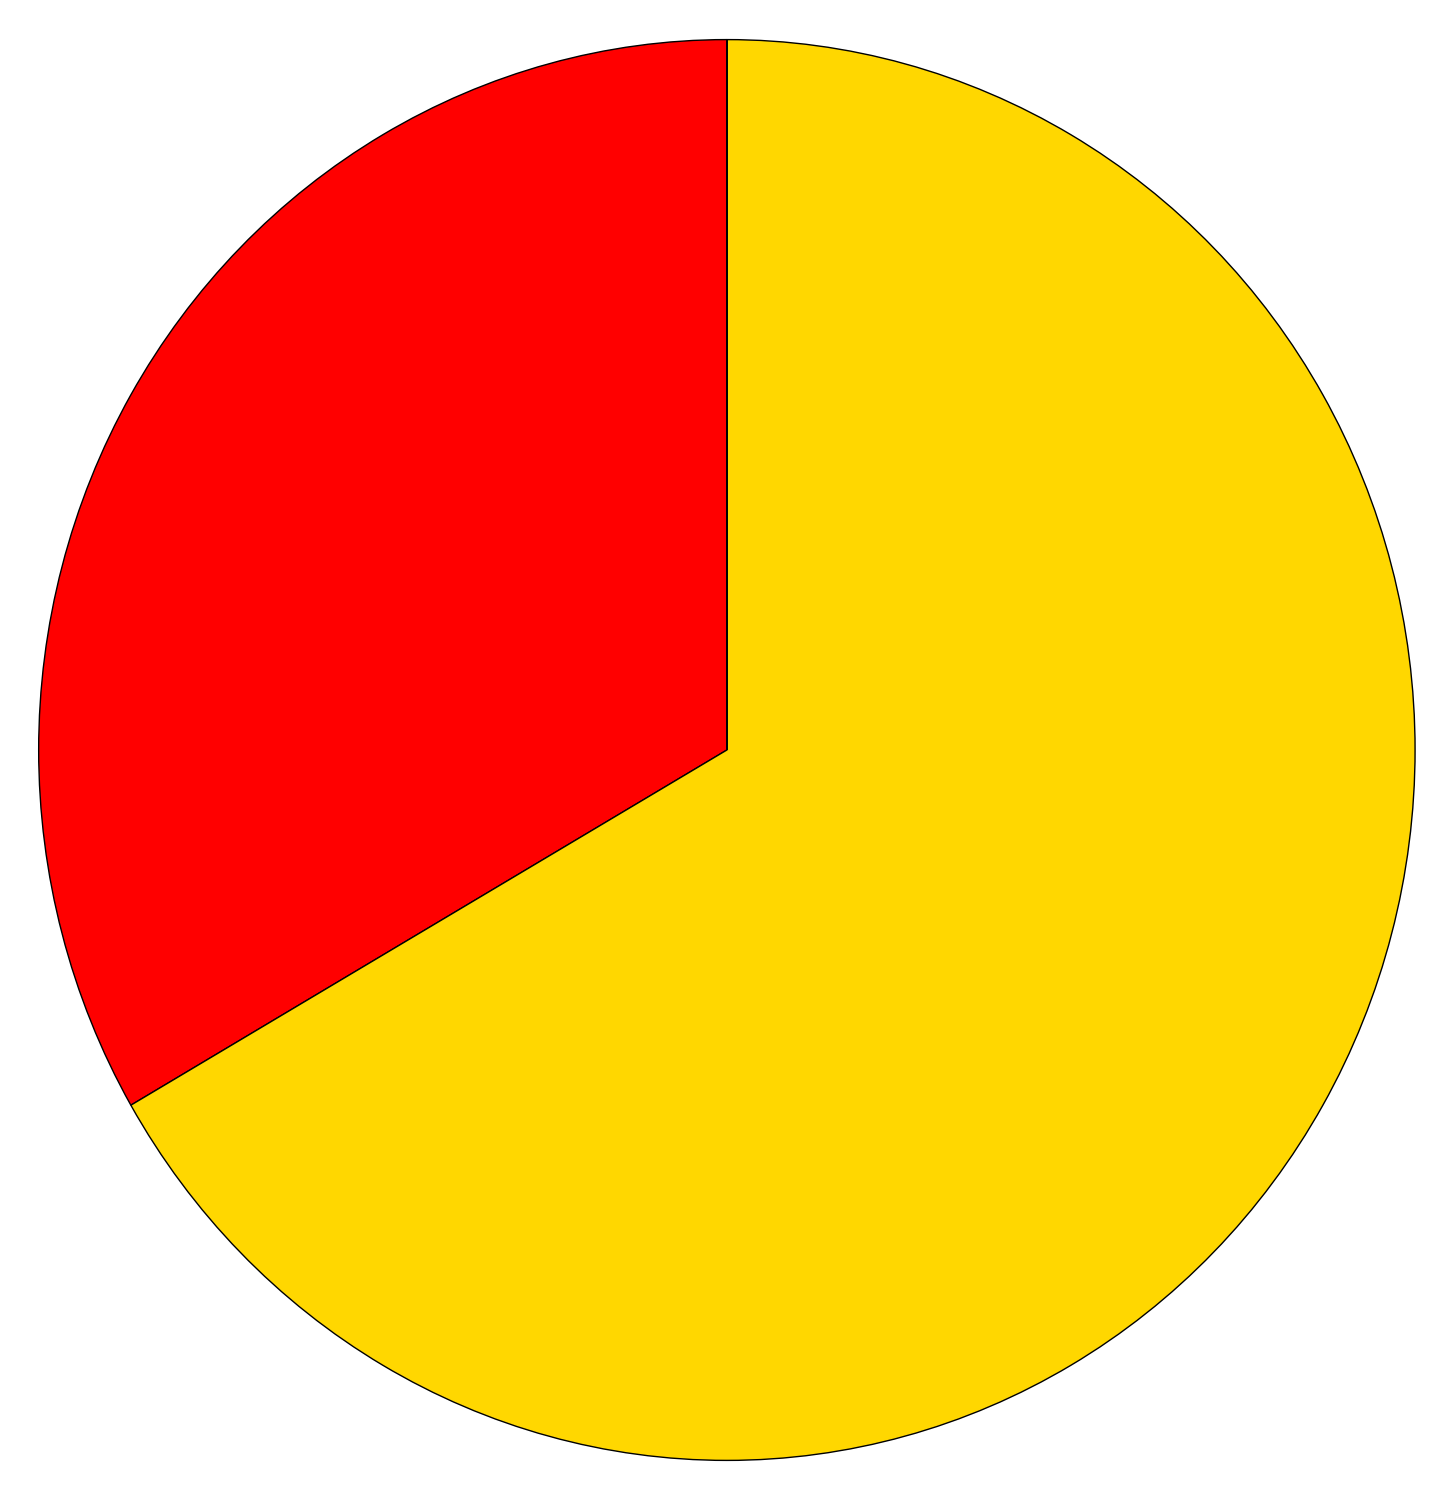
\includegraphics[width=\textwidth]{valenceALLL2gen}
    \caption{Ridge regression}
  \end{subfigure}
  
  \begin{subfigure}[b]{0.3\textwidth}
    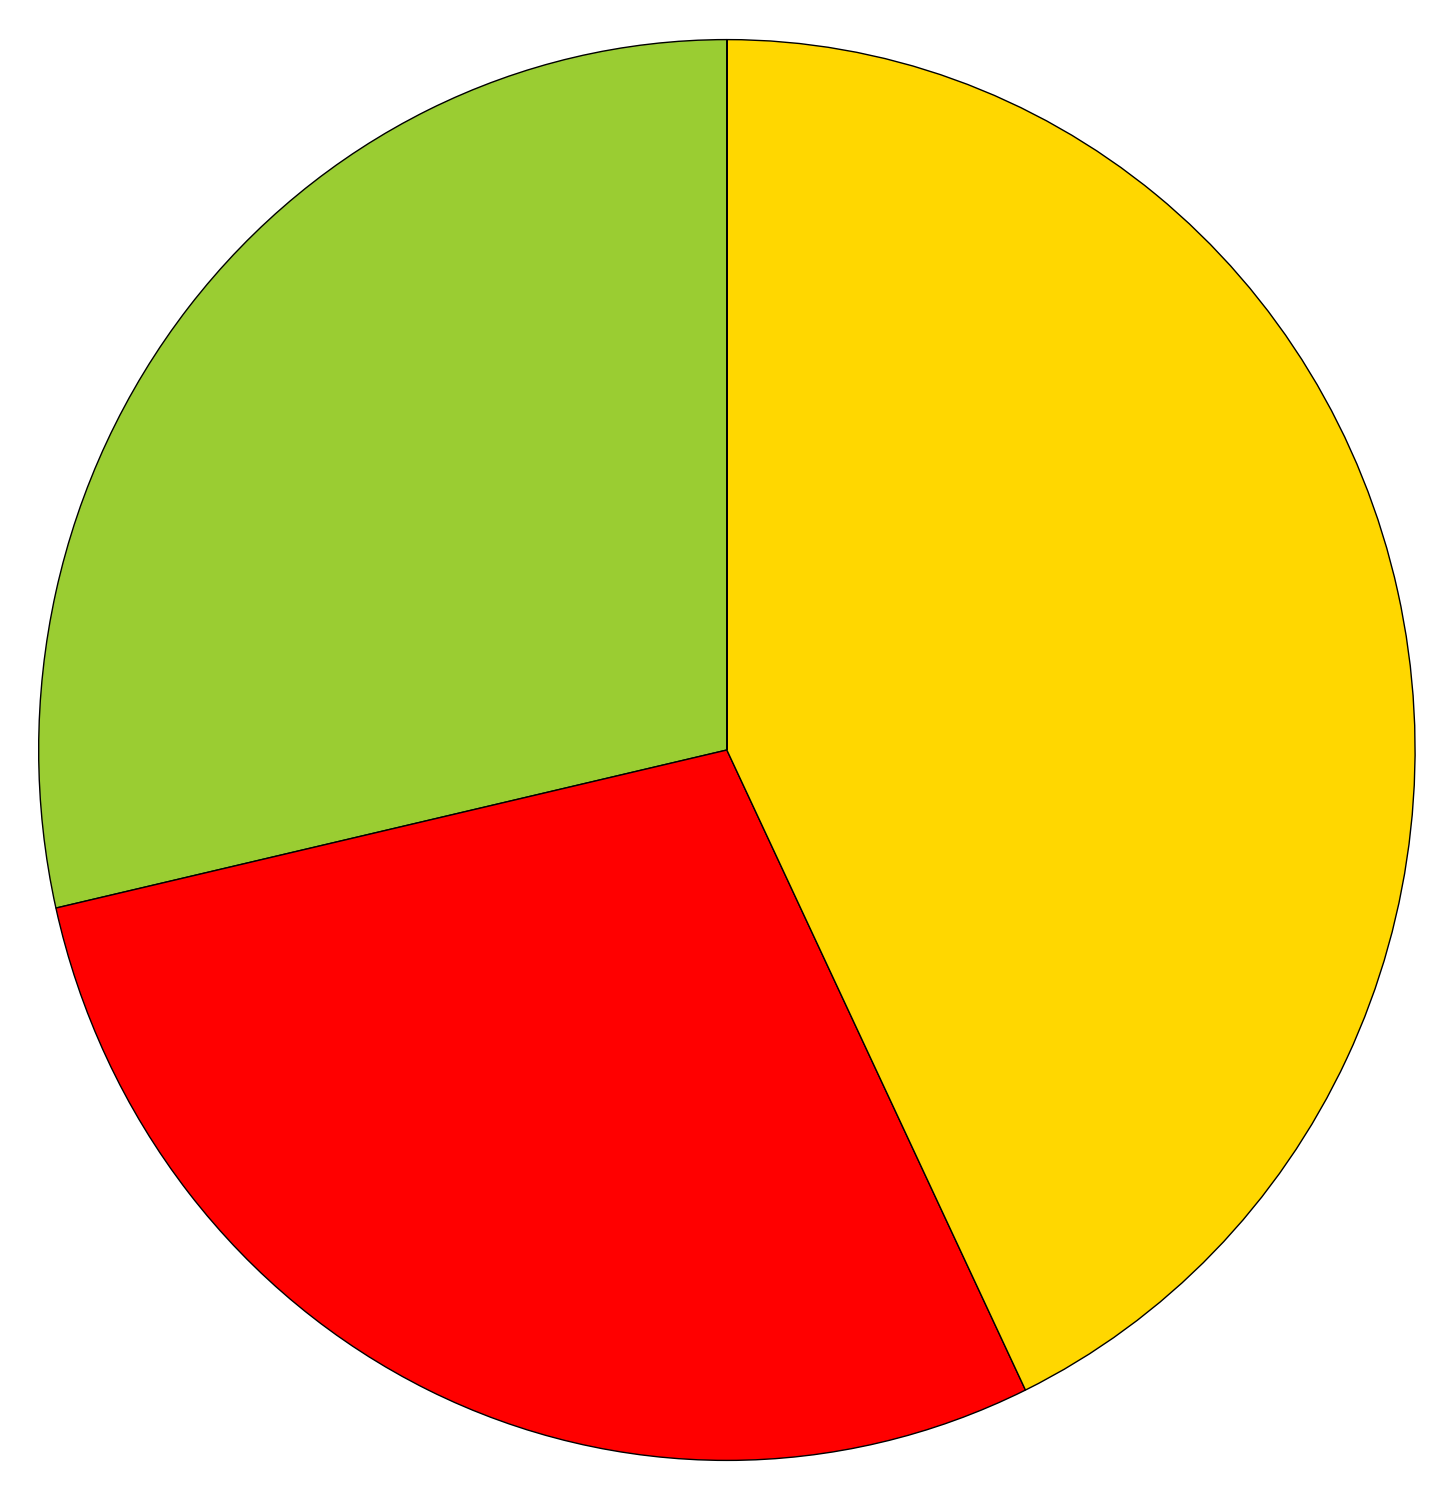
\includegraphics[width=\textwidth]{valenceALLRFgen}
    \caption{Random forests}
  \end{subfigure}
  \hfill
  \begin{subfigure}[b]{0.3\textwidth}
    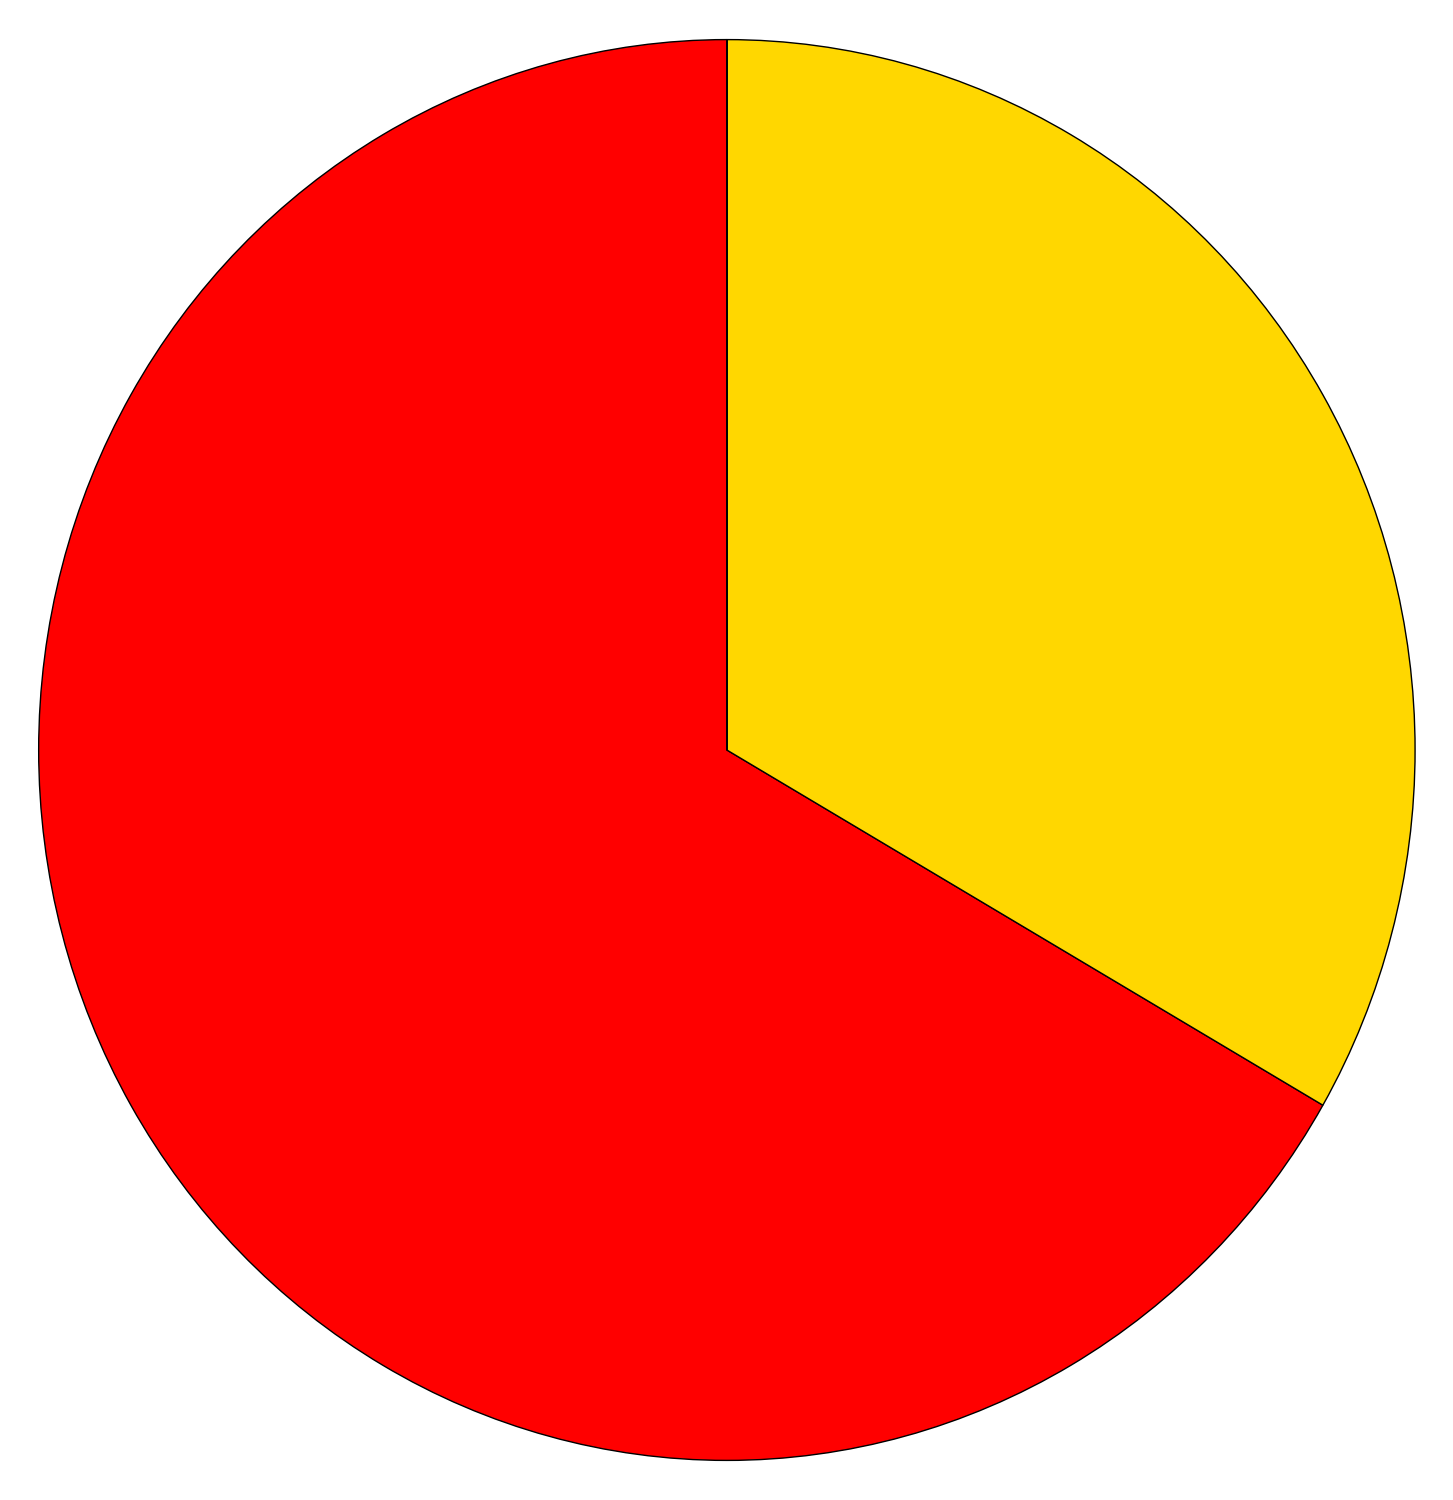
\includegraphics[width=\textwidth]{valenceALLPCAgen}
    \caption{PCA}
  \end{subfigure}
  \hfill
  \begin{subfigure}[b]{0.3\textwidth}
    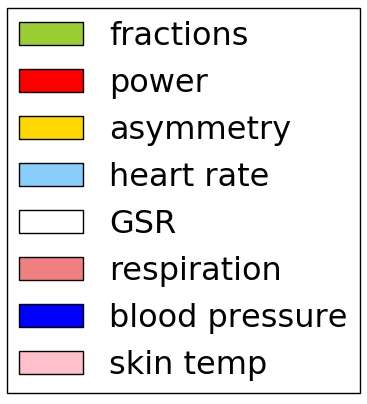
\includegraphics[width=\textwidth]{legend}
    \caption{Legend\label{valencepieslegendgen}}
  \end{subfigure}
\end{figure}
\clearpage

For arousal, it is clear that the EEG features are quite dominant. None the non-EEG features were selected. The EEG features themselves different from selection method to selection method. One possible explanation for this is that the accuracies of the models are not great. The models are thus not fitting very well. This may cause unstable behaviour in the less stable feature selection methods like linear regression , lasso regression, Pearson correlation, distance correlation, etc. The random forest method is the most advanced feature selection method and it gives a small preference to asymmetry features. This concurs with the finding in the personal specific setting. Similar things can be observed for valence. Again, the asymmetry features are preferred by the random forest, which concurs with the literature and similar studies. It might be important to note that there is a high correlation between asymmetry and the valence, which is visible when looking at the Pearson correlation output.

\npar

To further look at the difference between EEG and non-EEG features, the random forest selection method was again used three times. The first time, all features were available. The second time, only EEG features were available and the third time, only non-EEG features. The results are shown in Figure \ref{arousalphyeegall_gen}, for arousal and Figure \ref{valencephyeegall_gen} for valence. The exact values are shown in Table \ref{phyeegallgenTable}


\mijnfiguur{width=1.\textwidth}{arousalphyeegall_gen}{The performance of arousal prediction for all, EEG and non-EEG features in a cross-subject setting.}

\mijnfiguur{width=1.\textwidth}{valencephyeegall_gen}{The performance of valence prediction for all, EEG and non-EEG features in a cross-subject setting.}

\begin{table}[H]
\centering
\begin{tabular}{lll}
\textbf{} & \textbf{arousal} & \textbf{valence} \\
\textbf{feat set}  & \textbf{avg acc}       & \textbf{avg acc}          \\
\textbf{all}       & 0.6344           & 0.5531           \\
\textbf{EEG}       & 0.6094           & 0.5656           \\
\textbf{non-EEG}   & 0.6344           & 0.5531          
\end{tabular}
\caption{The test accuracies for both arousal and valence, using different feature sets.\label{phyeegallgenTable}}
\end{table}

Comparing Table \ref{phyeegallgenTable} with Table \ref{phyeegalltable}, one can see that the difference in accuracy between non-EEG features and all and/or EEG features only is much smaller. This is an indication that the non-EEG features might work better in a cross subject setting. The reason that the feature selection methods select only EEG features might be due to the fact there are more EEG features available. Given that EEG features often contain a lot of noise, chances are that the selection methods are able to find EEG features that fit the limit sample set well. 

\npar

To find out which non-EEG feature might be useful, the selected non-EEG features from the random forest selection method were analysed. Again one can observe that the selected features for each feature selected method are quite different. The random focus seems to prefer skin temperature, heart rate and GSR for arousal and blood pressure combined with GSR for valence.

\clearpage

\begin{figure}[!tbp]
  \centering
  \caption{Selection features for arousal classification, using only non-EEG features in a cross-subject setting.\label{arousalnon-EEGpiesgen}}
  \begin{subfigure}[b]{0.3\textwidth}
    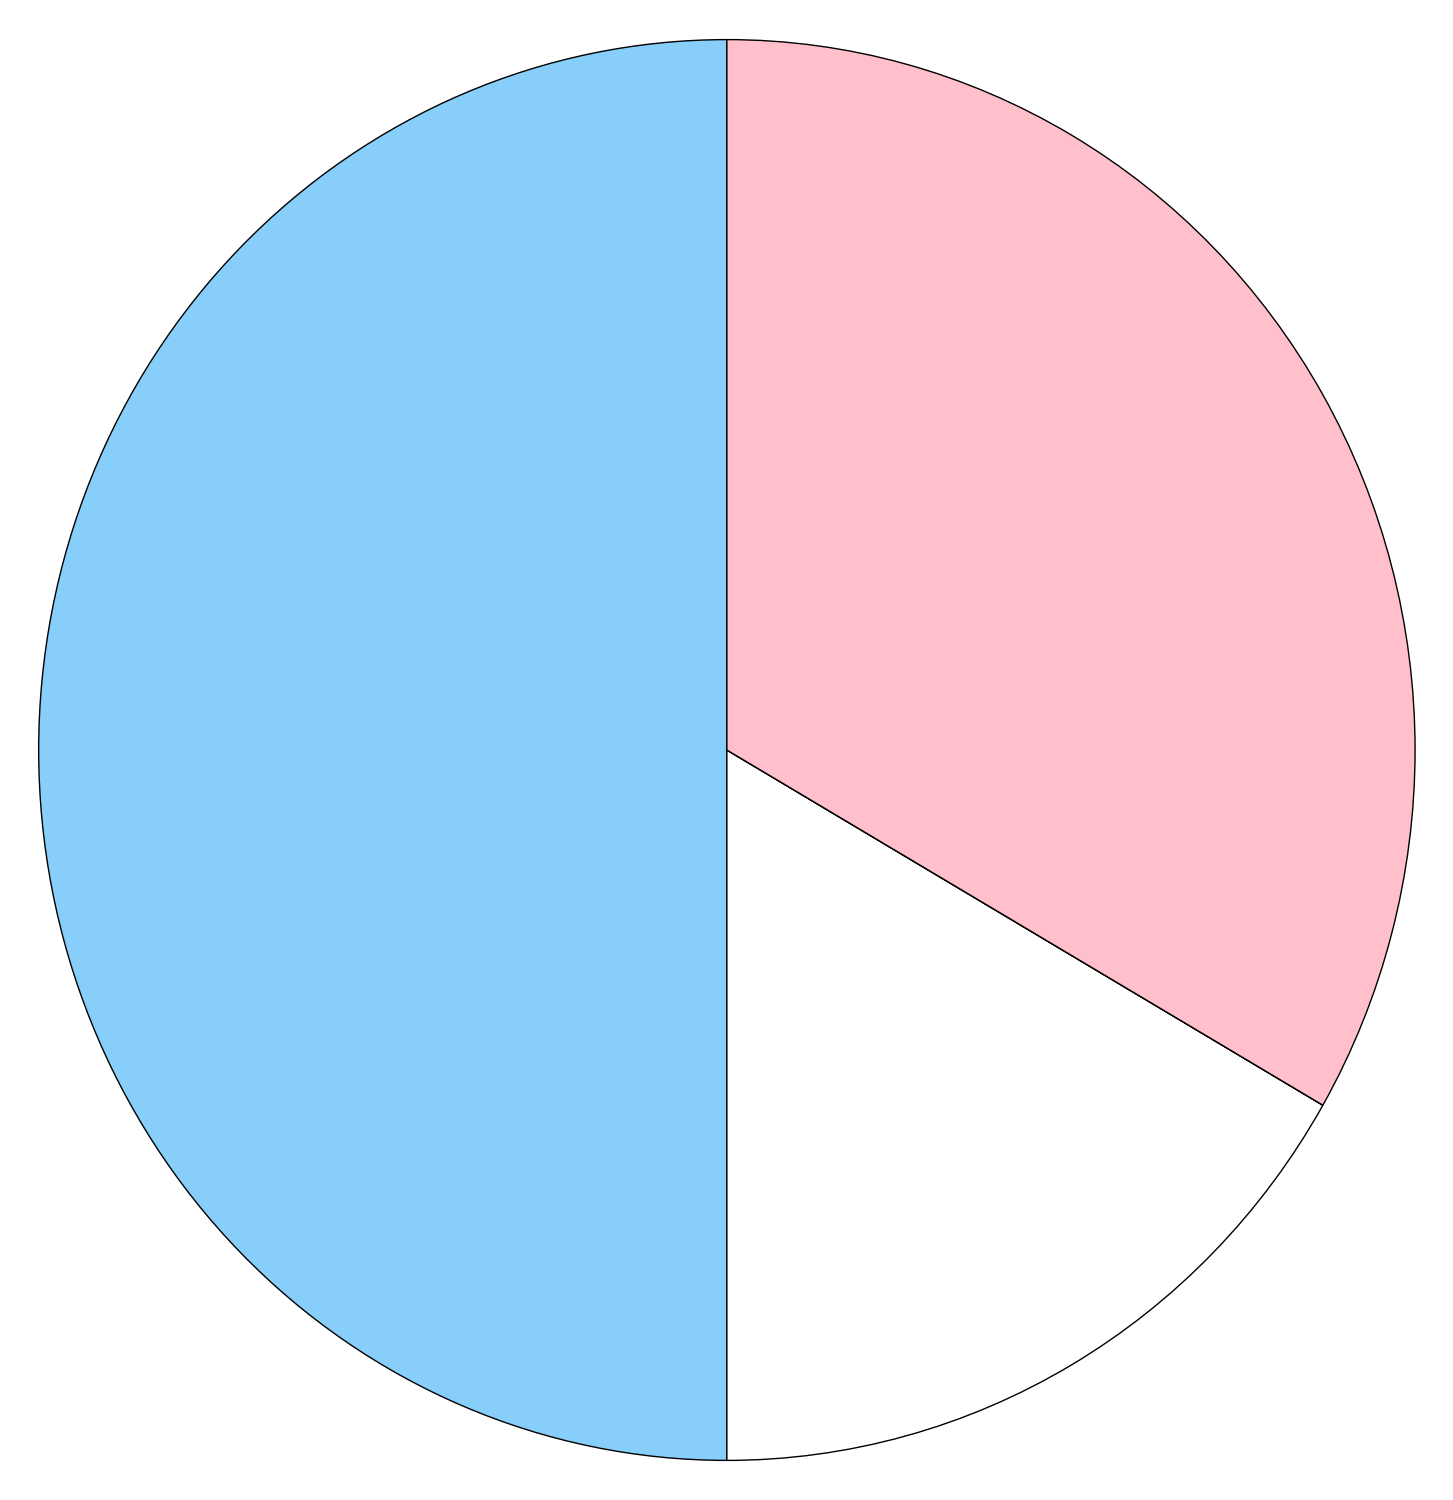
\includegraphics[width=\textwidth]{arousalnon-EEGpearsonRgen}
    \caption{Pearson correlation}
  \end{subfigure}
  \hfill
  \begin{subfigure}[b]{0.3\textwidth}
    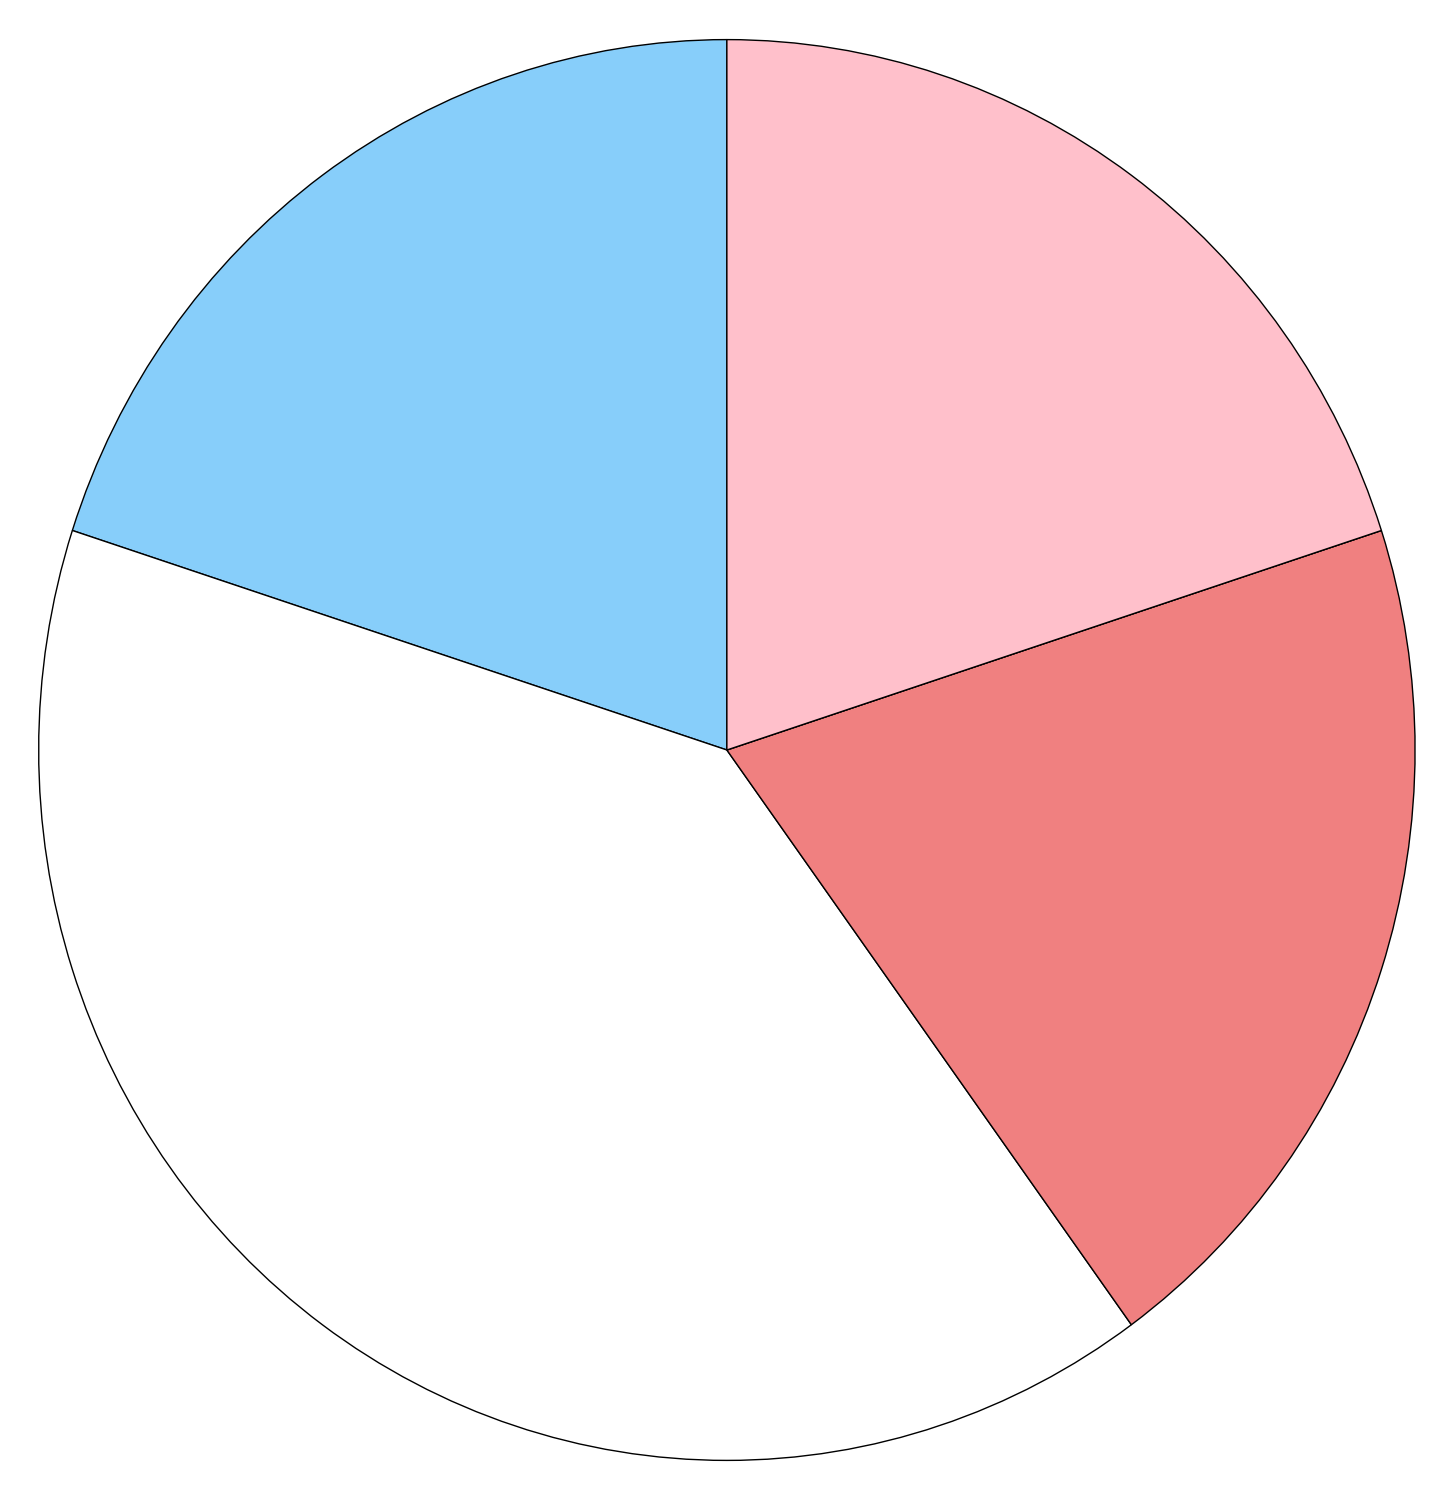
\includegraphics[width=\textwidth]{arousalnon-EEGMutInfgen}
    \caption{Mutual information}
  \end{subfigure}
  \hfill
  \begin{subfigure}[b]{0.3\textwidth}
    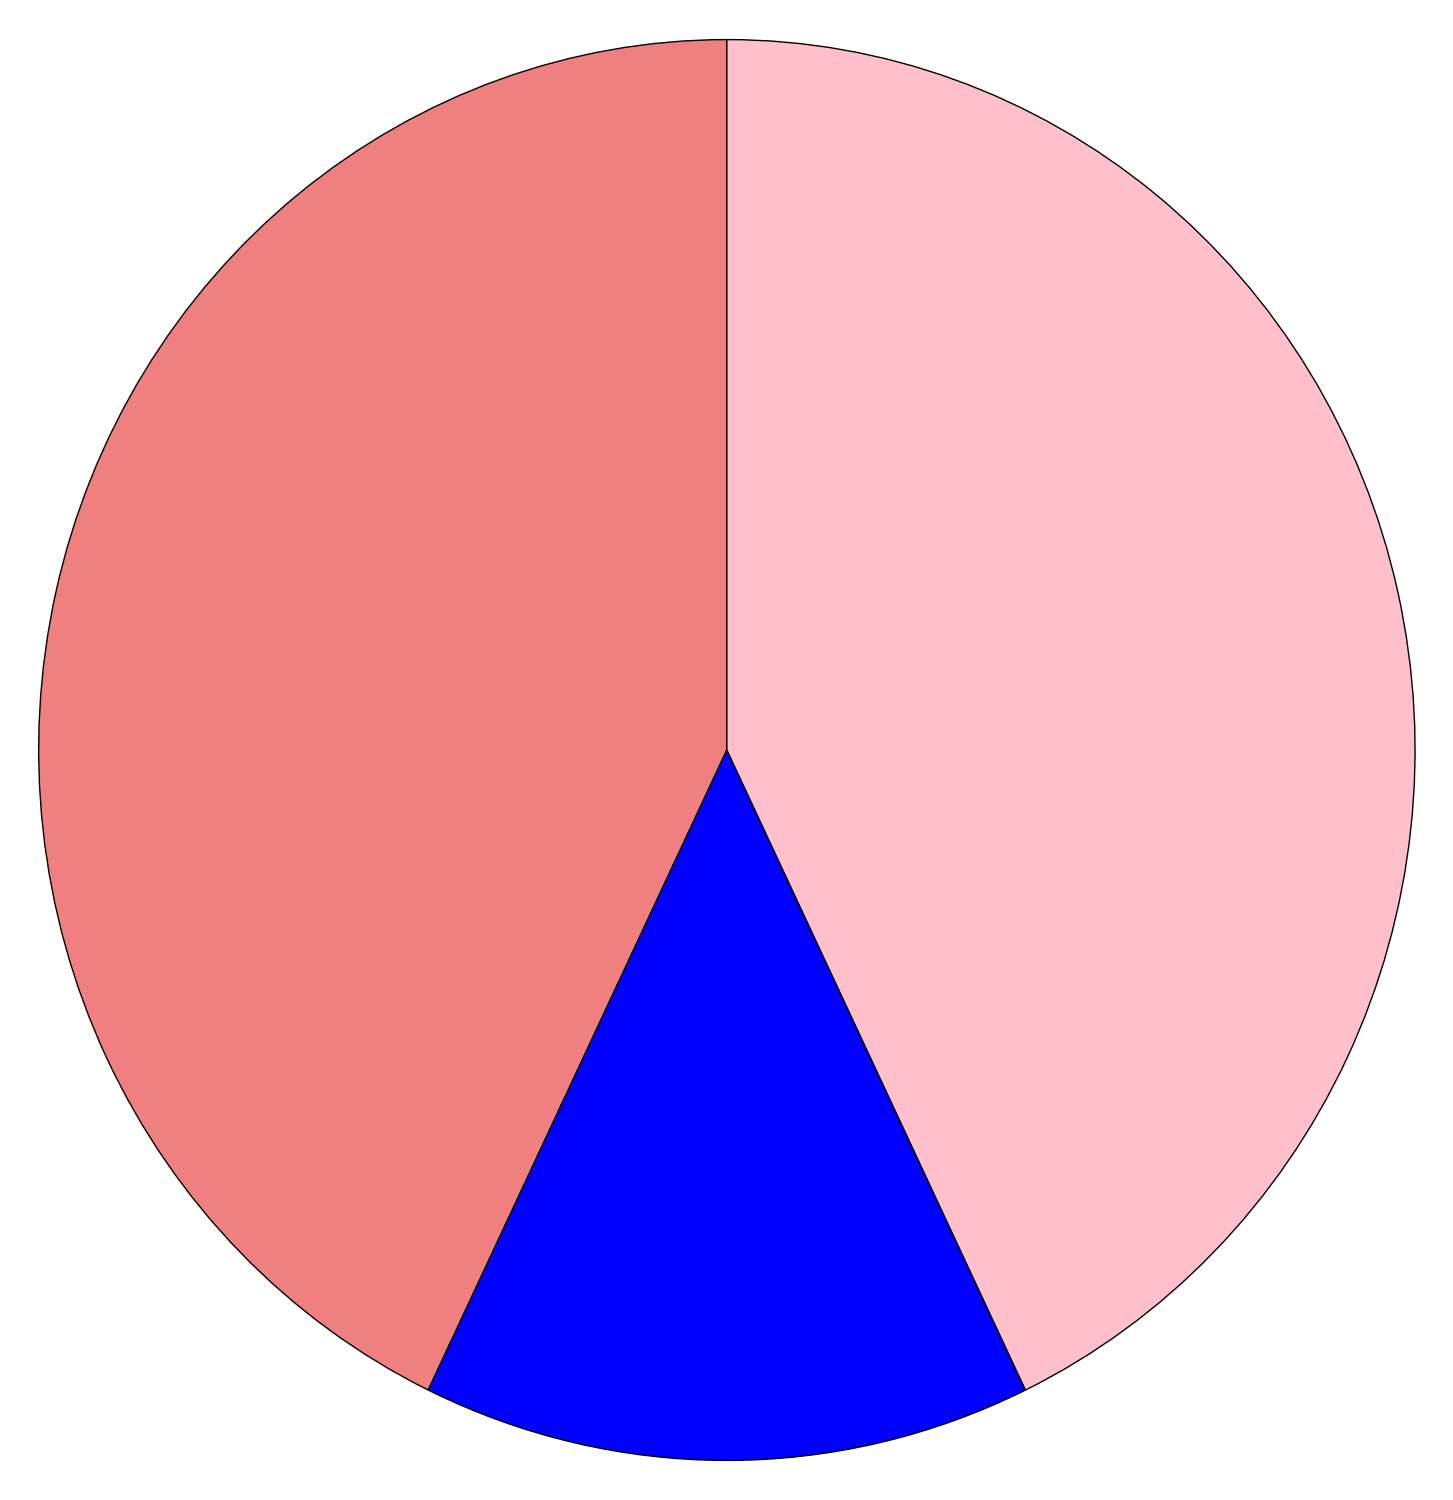
\includegraphics[width=\textwidth]{arousalnon-EEGdCorrgen}
    \caption{Distance Correlation}
  \end{subfigure}
  
  \begin{subfigure}[b]{0.3\textwidth}
    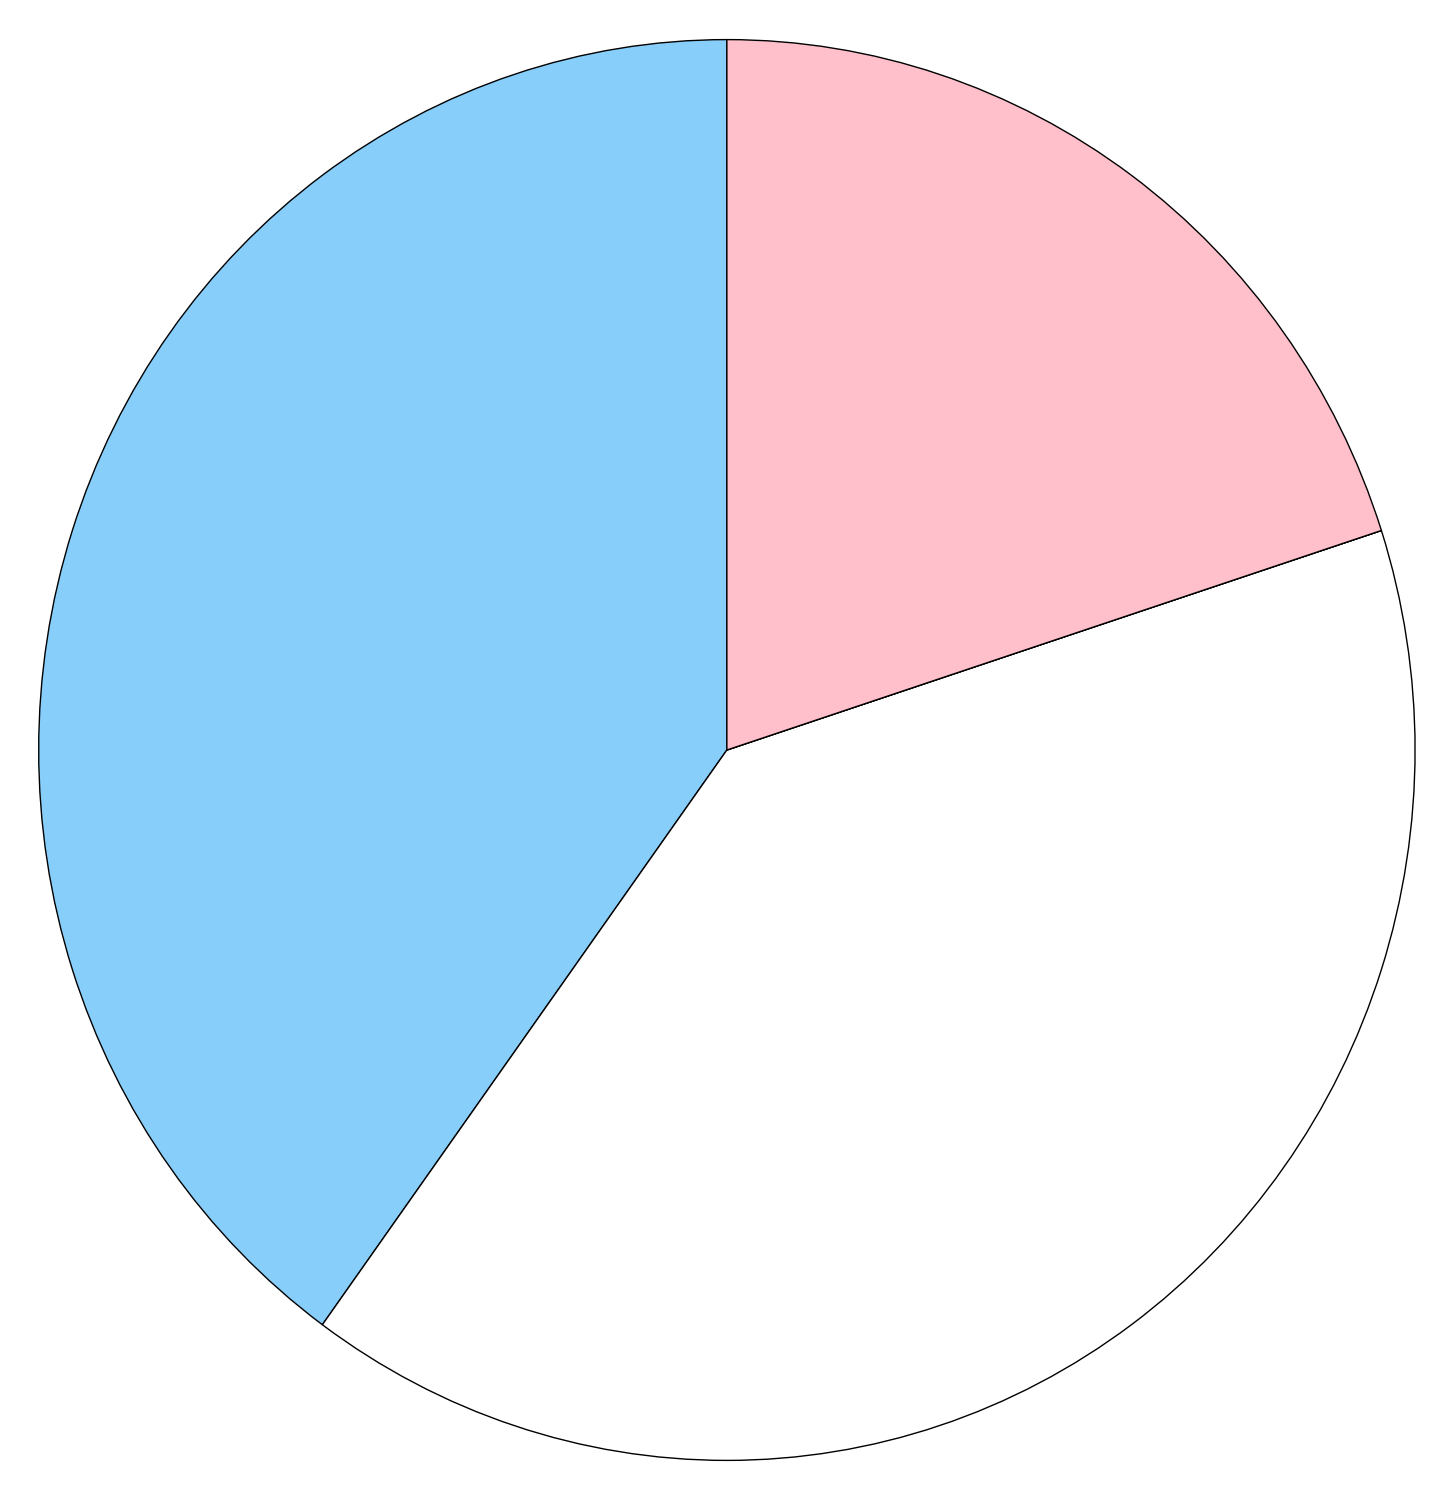
\includegraphics[width=\textwidth]{arousalnon-EEGANOVAgen}
    \caption{ANOVA}
  \end{subfigure}
  \hfill
  \begin{subfigure}[b]{0.3\textwidth}
    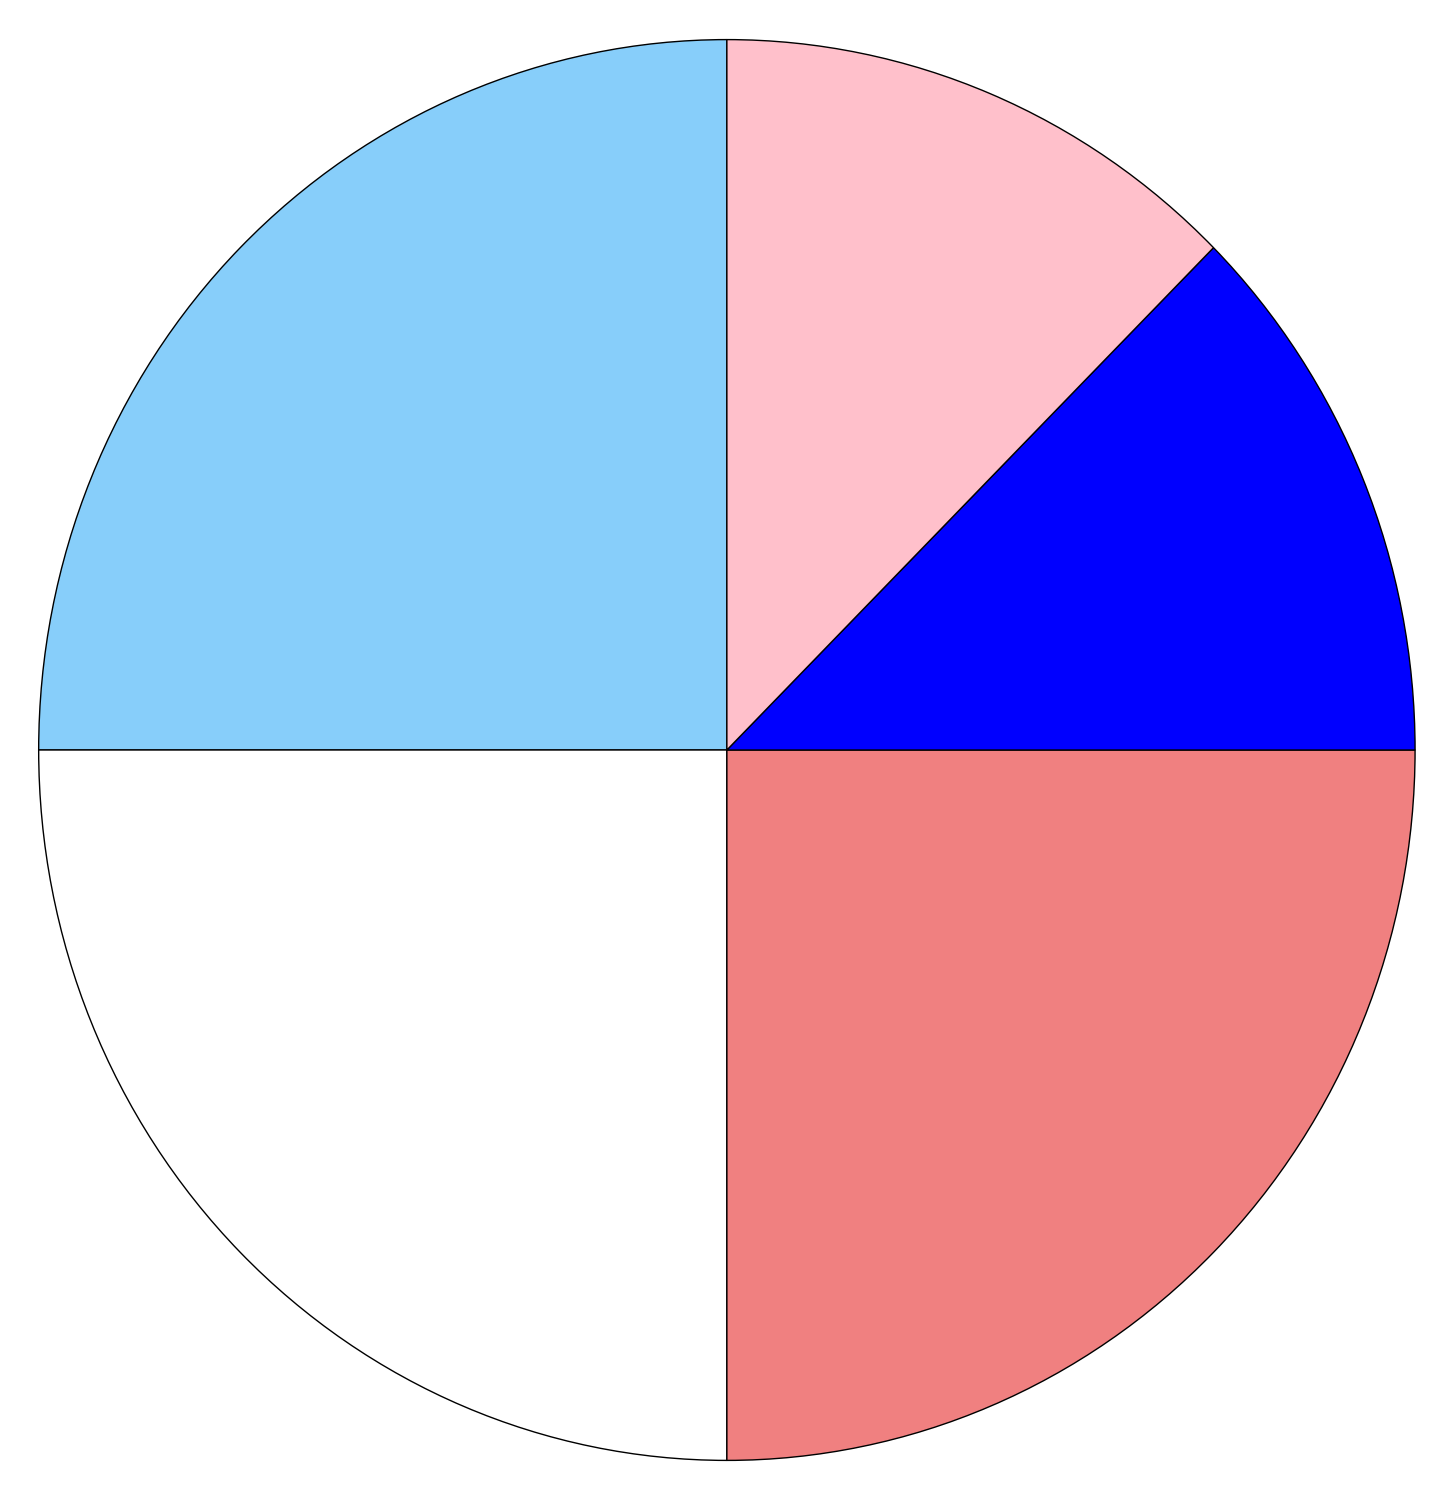
\includegraphics[width=\textwidth]{arousalnon-EEGLRgen}
    \caption{Linear regression}
  \end{subfigure}
  \hfill
  \begin{subfigure}[b]{0.3\textwidth}
    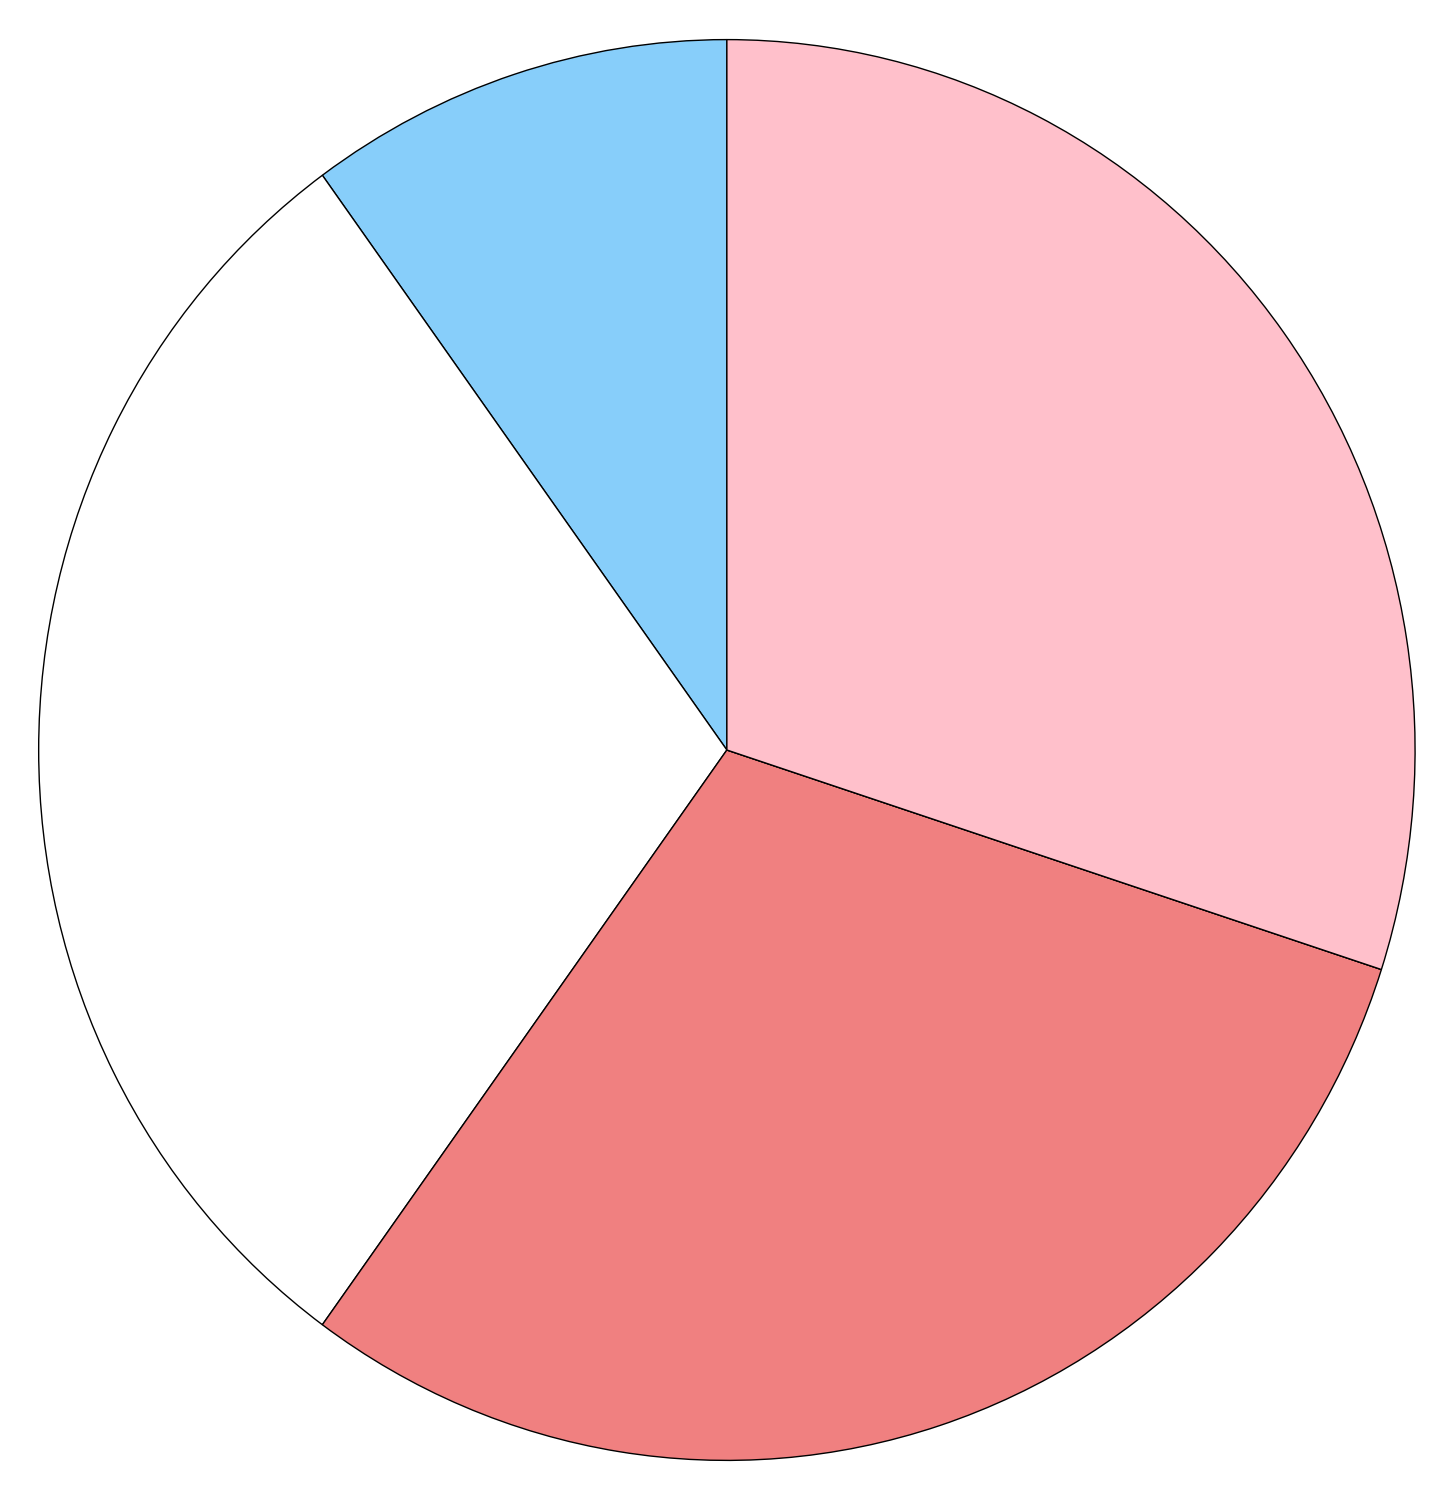
\includegraphics[width=\textwidth]{arousalnon-EEGSVMgen}
    \caption{SVM}
  \end{subfigure}
  
  \begin{subfigure}[b]{0.3\textwidth}
    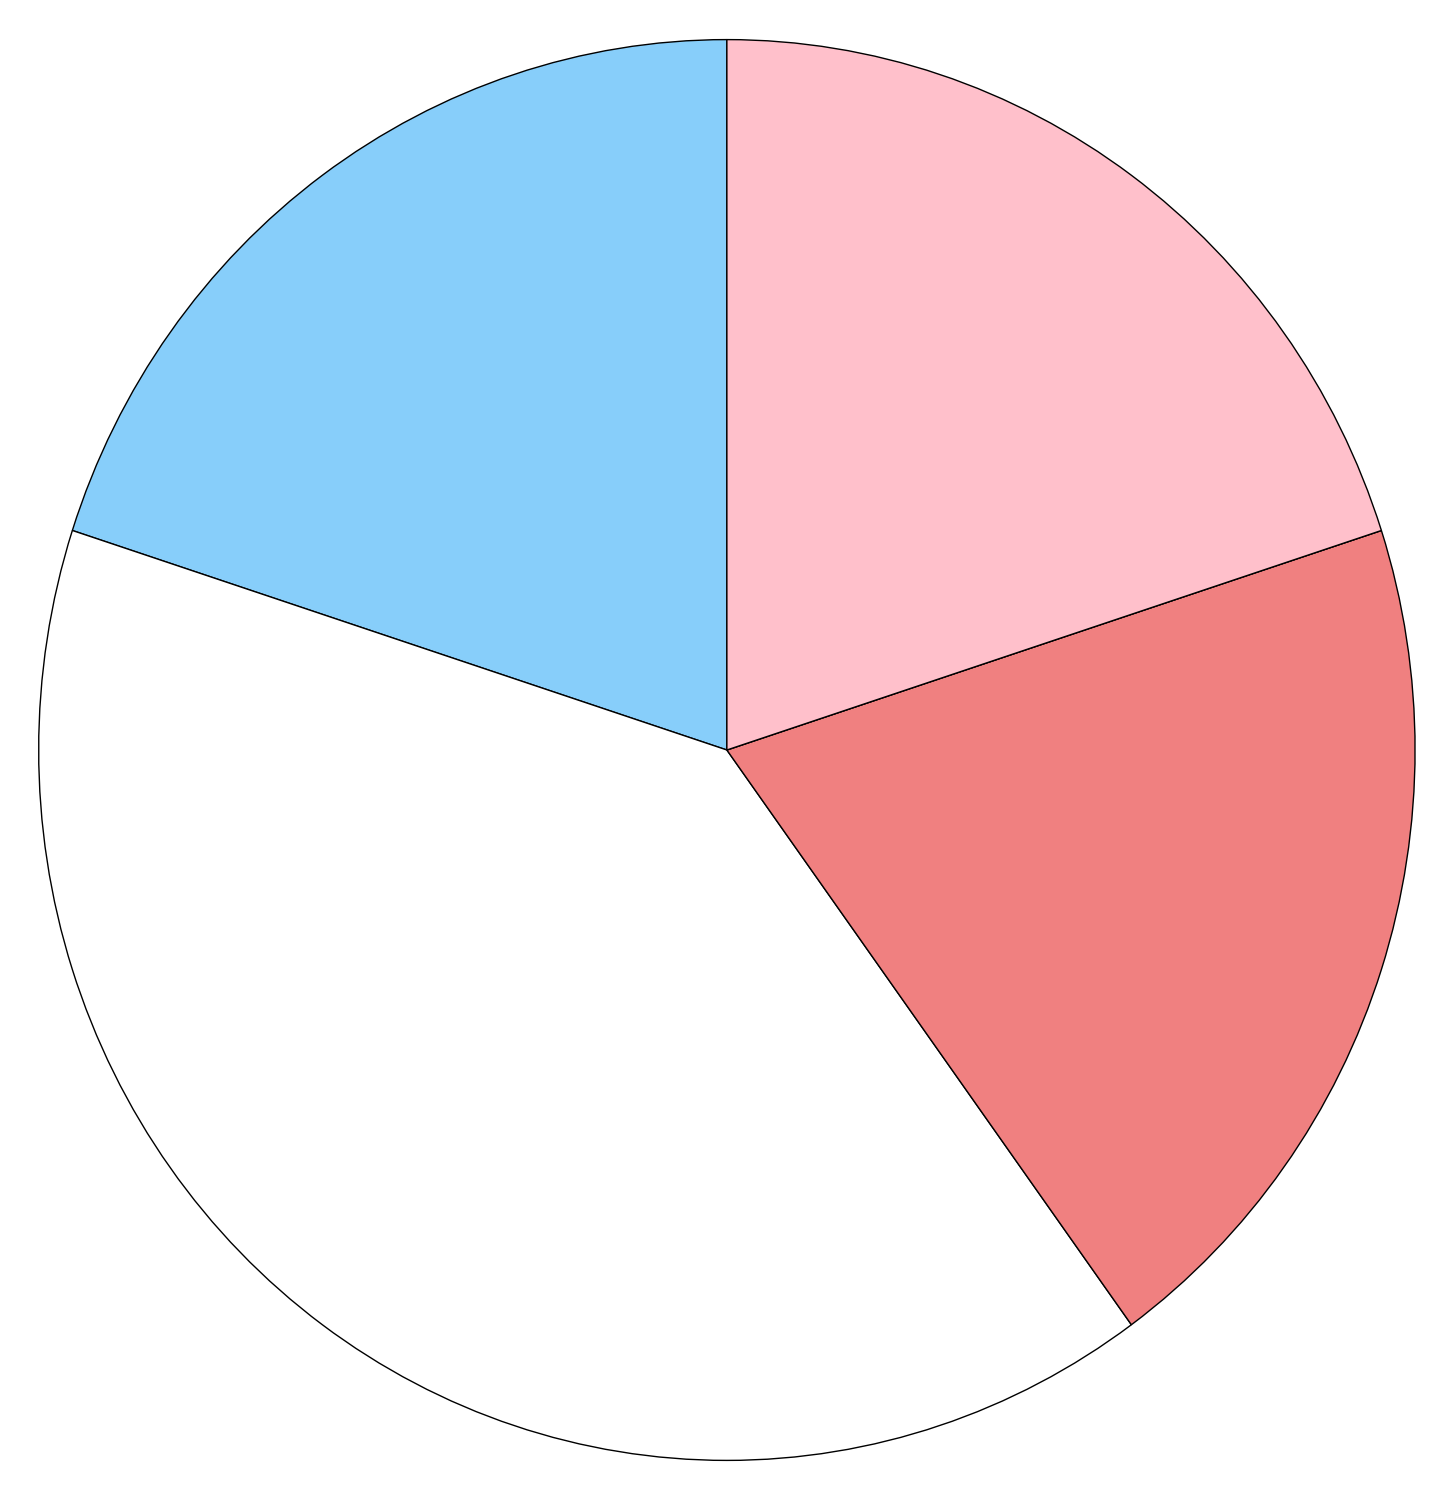
\includegraphics[width=\textwidth]{arousalnon-EEGLDAgen}
    \caption{LDA}
  \end{subfigure}
  \hfill
  \begin{subfigure}[b]{0.3\textwidth}
    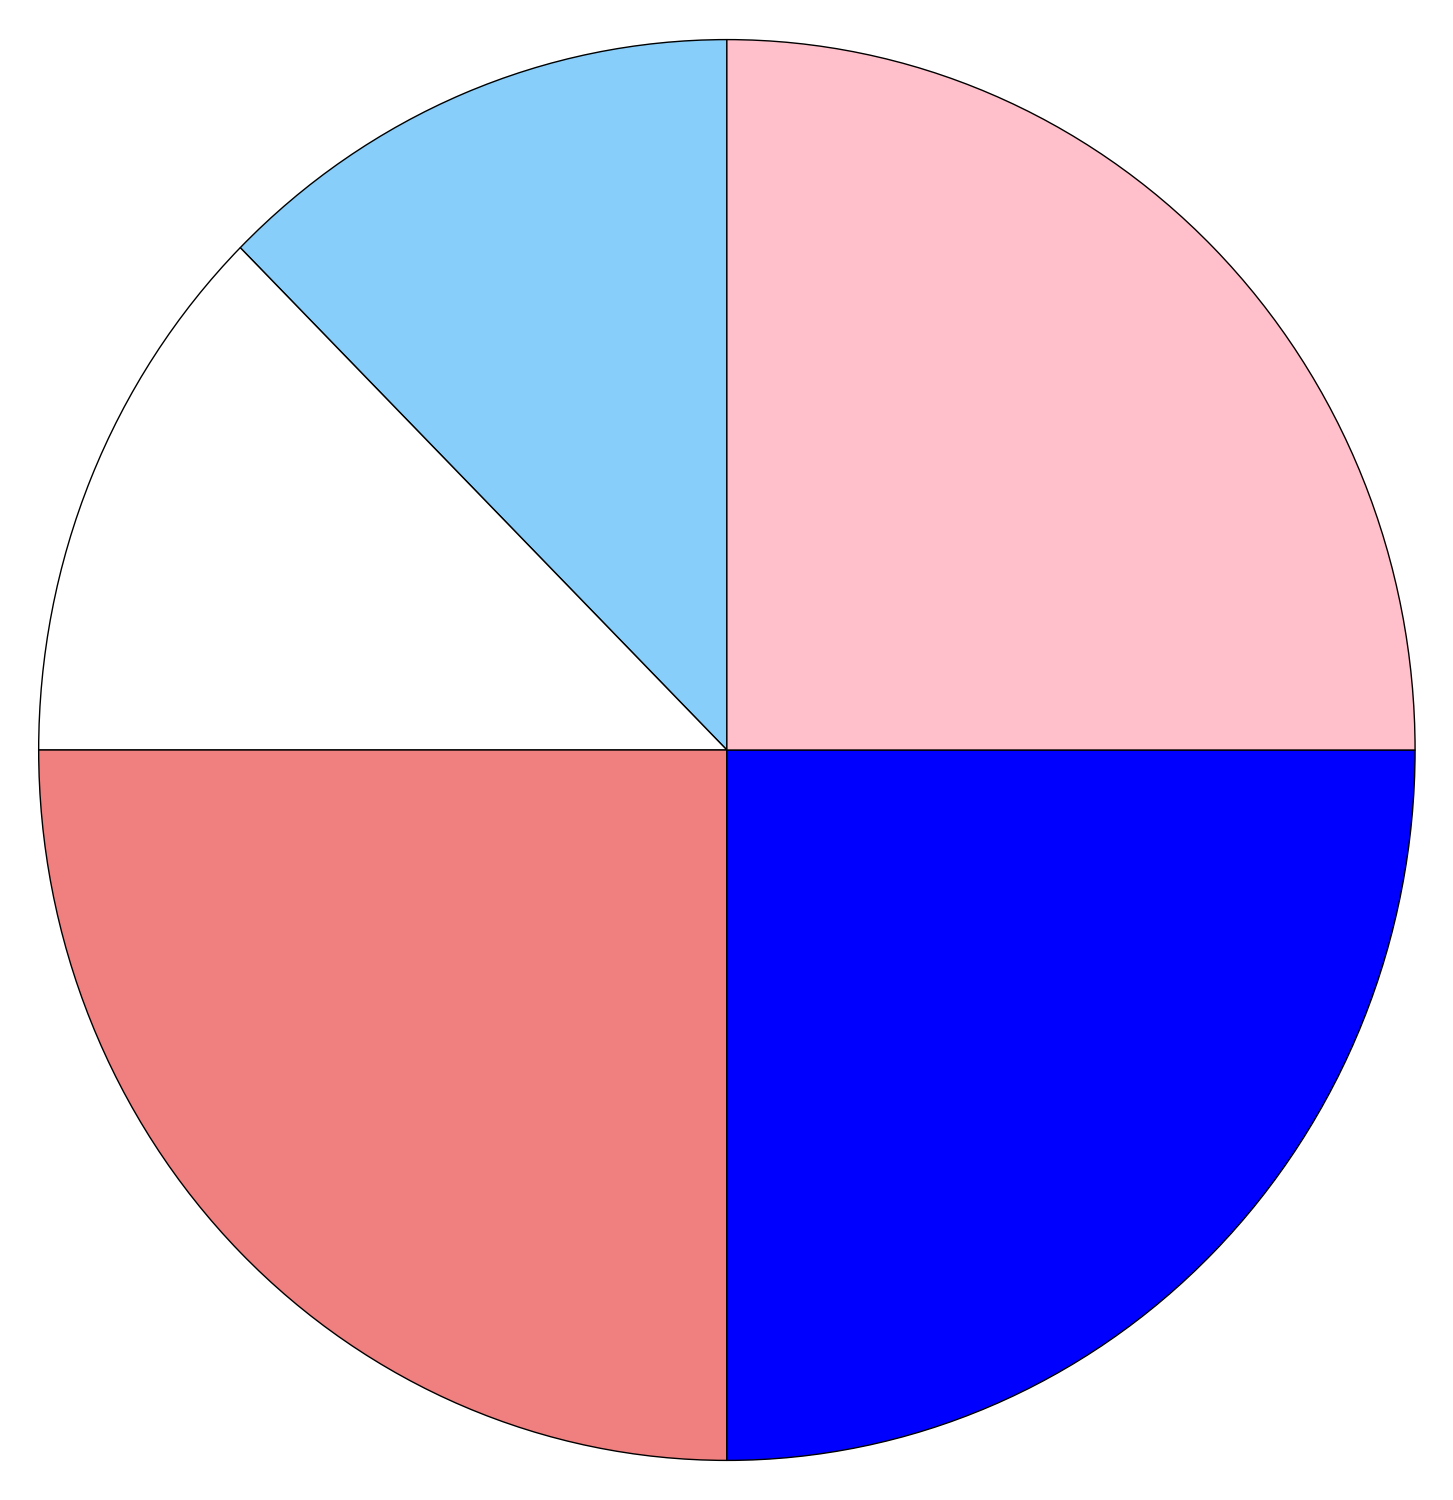
\includegraphics[width=\textwidth]{arousalnon-EEGL1gen}
    \caption{Lasso regression}
  \end{subfigure}
  \hfill
  \begin{subfigure}[b]{0.3\textwidth}
    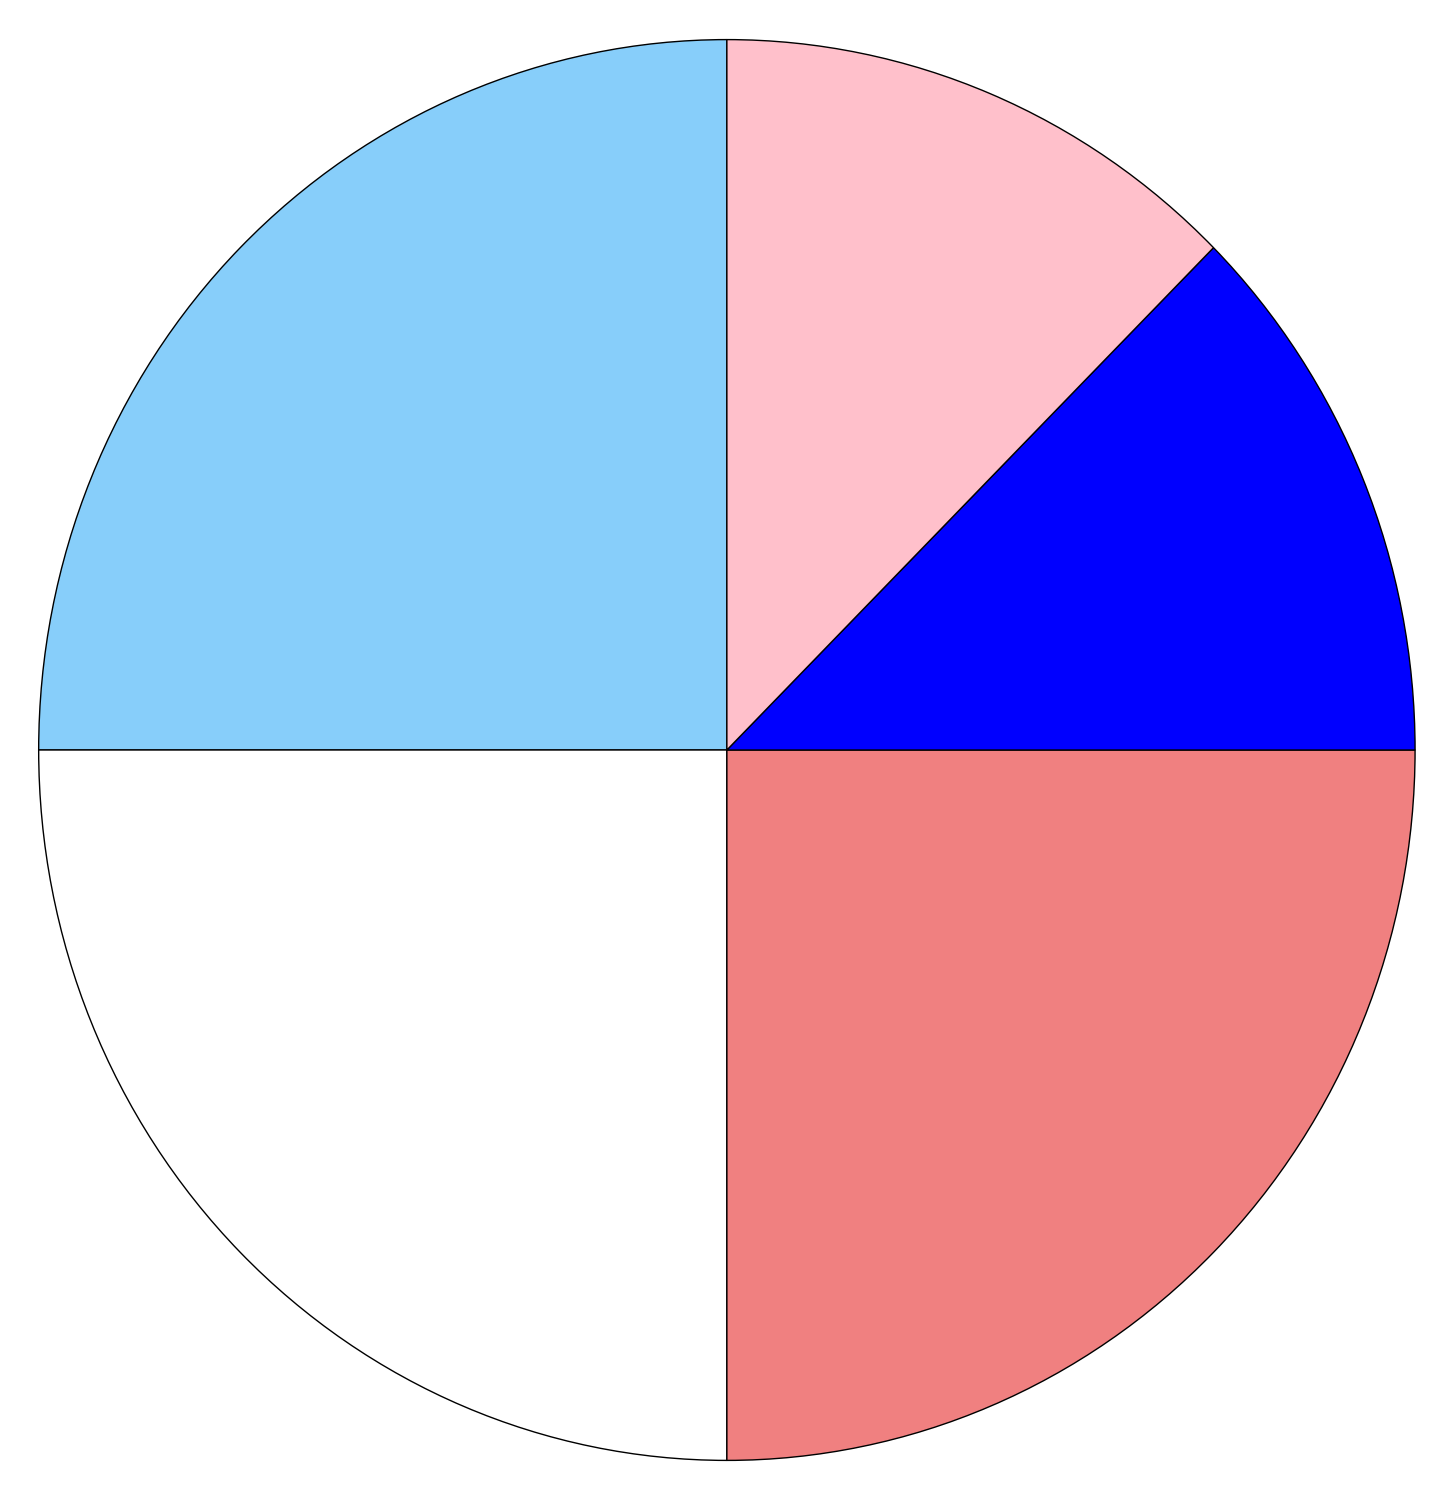
\includegraphics[width=\textwidth]{arousalnon-EEGL2gen}
    \caption{Ridge regression}
  \end{subfigure}
  
  \begin{subfigure}[b]{0.3\textwidth}
    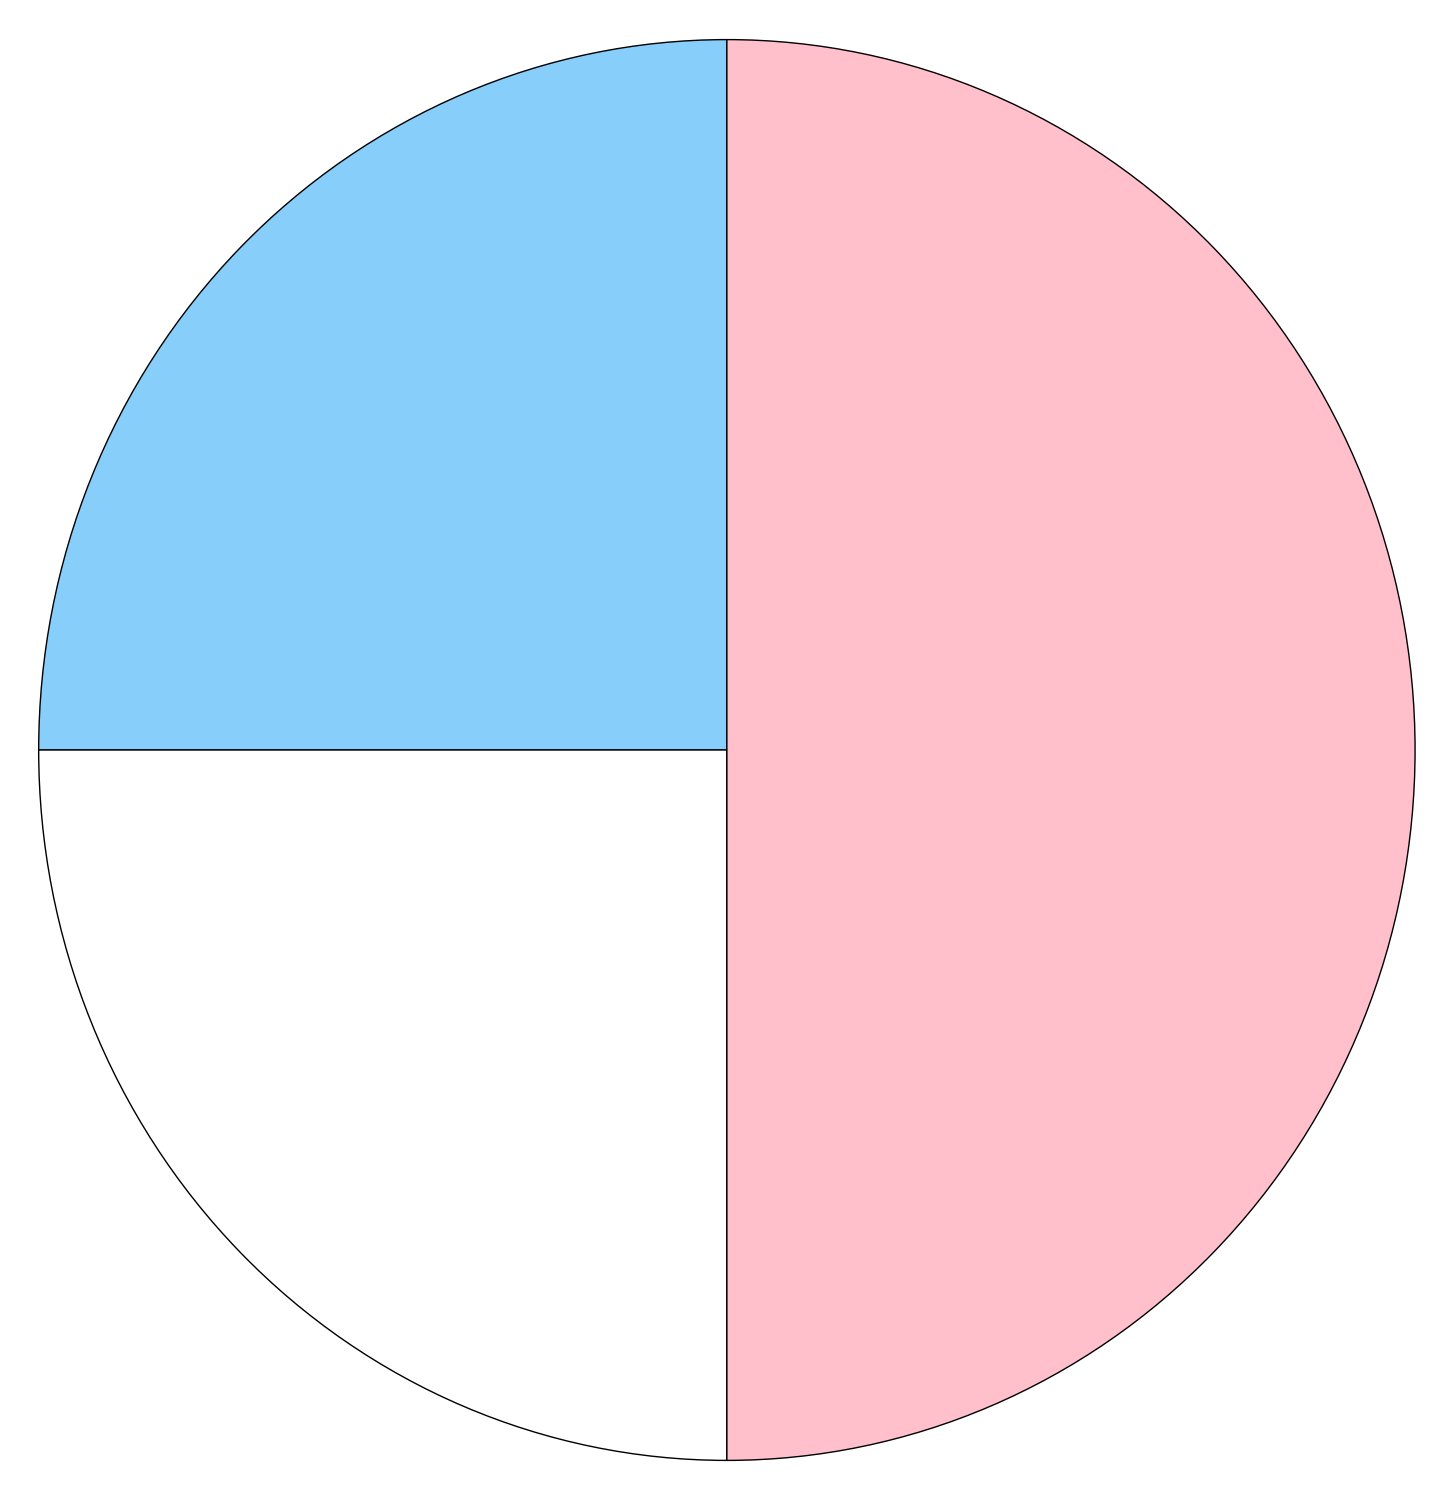
\includegraphics[width=\textwidth]{arousalnon-EEGRFgen}
    \caption{Random forests}
  \end{subfigure}
  \hfill
  \begin{subfigure}[b]{0.3\textwidth}
    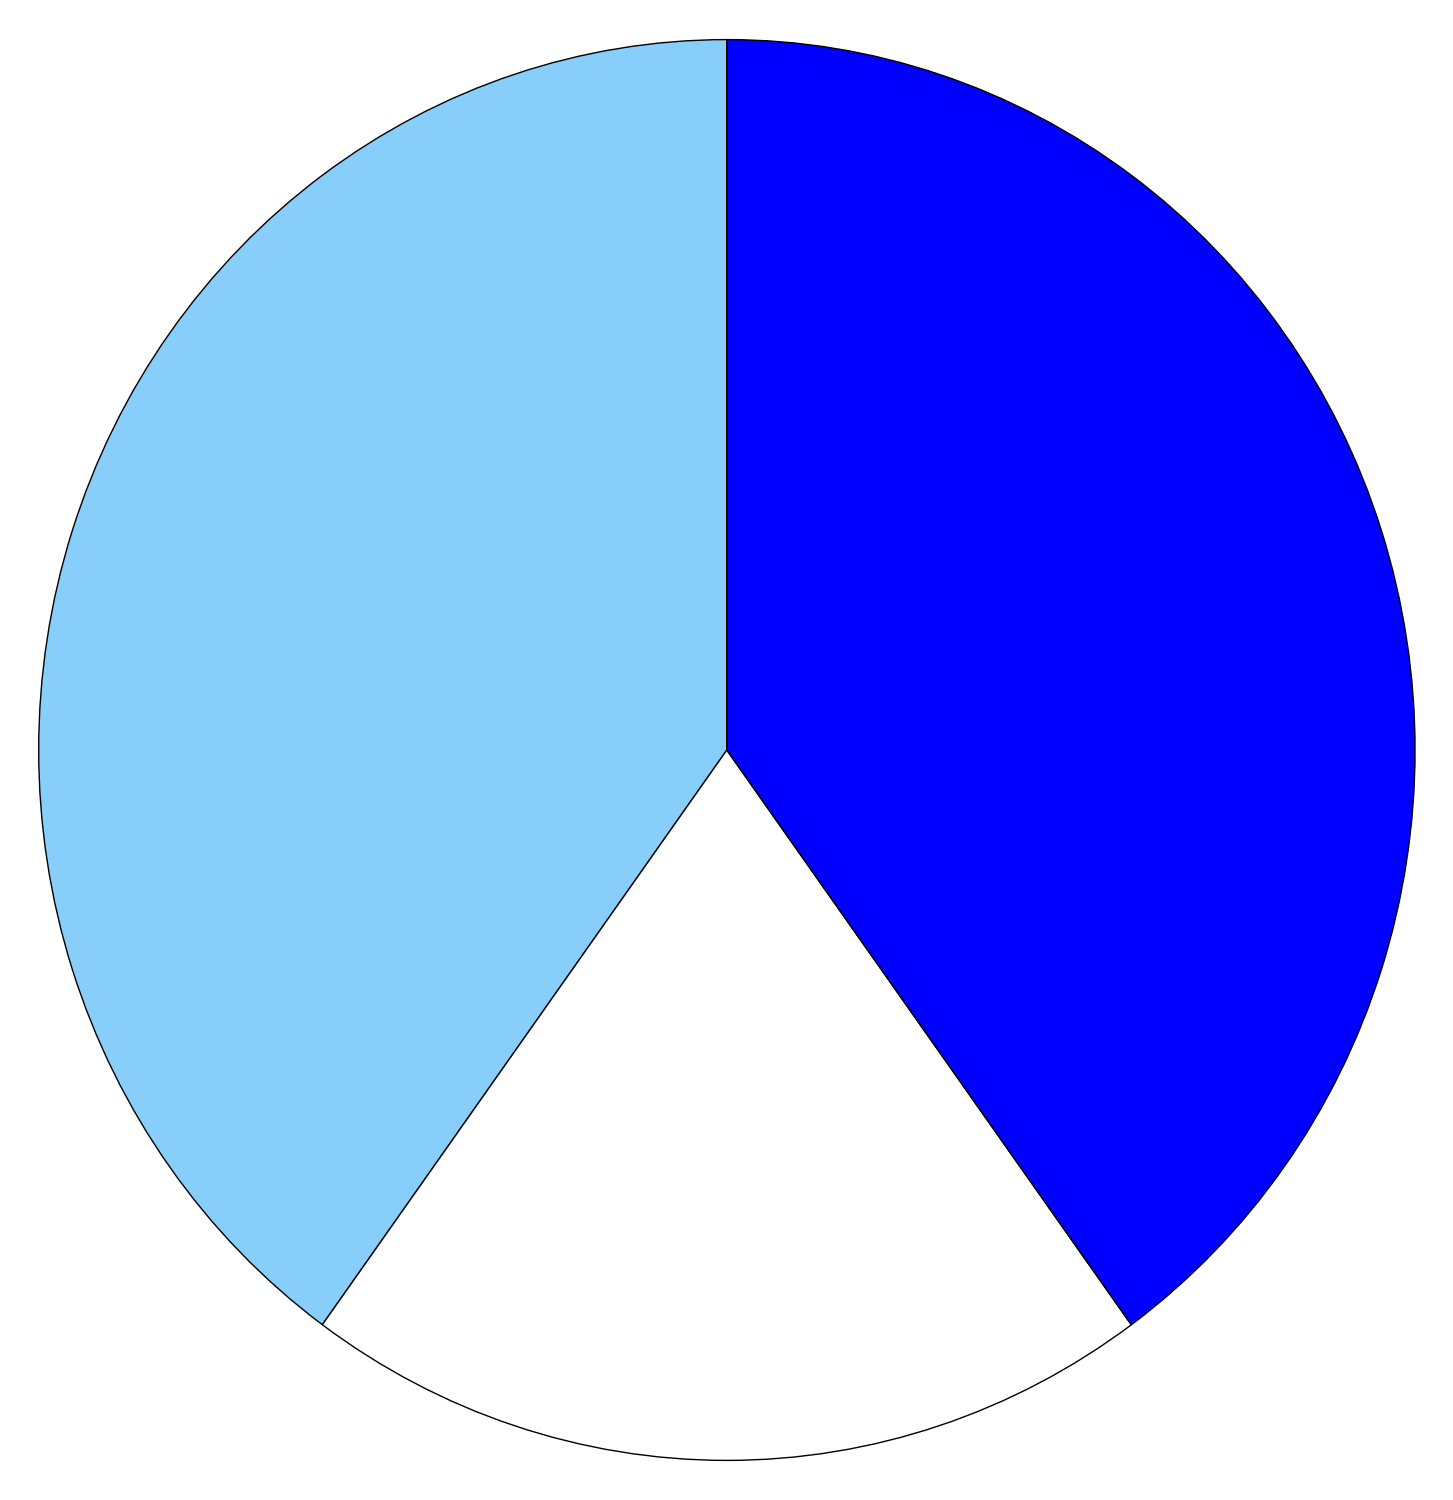
\includegraphics[width=\textwidth]{arousalnon-EEGPCAgen}
    \caption{PCA}
  \end{subfigure}
  \hfill
  \begin{subfigure}[b]{0.3\textwidth}
    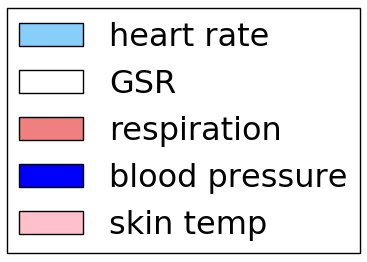
\includegraphics[width=\textwidth]{non-EEGlegend}
    \caption{Legend\label{arousalpiesnon-EEGlegendgen}}
  \end{subfigure}
\end{figure}

\clearpage

\begin{figure}[!tbp]
  \centering
  \caption{Selection features for valence classification, using only non-EEG features in a cross-subject setting.\label{valencenon-EEGpiesgen}}
  \begin{subfigure}[b]{0.3\textwidth}
    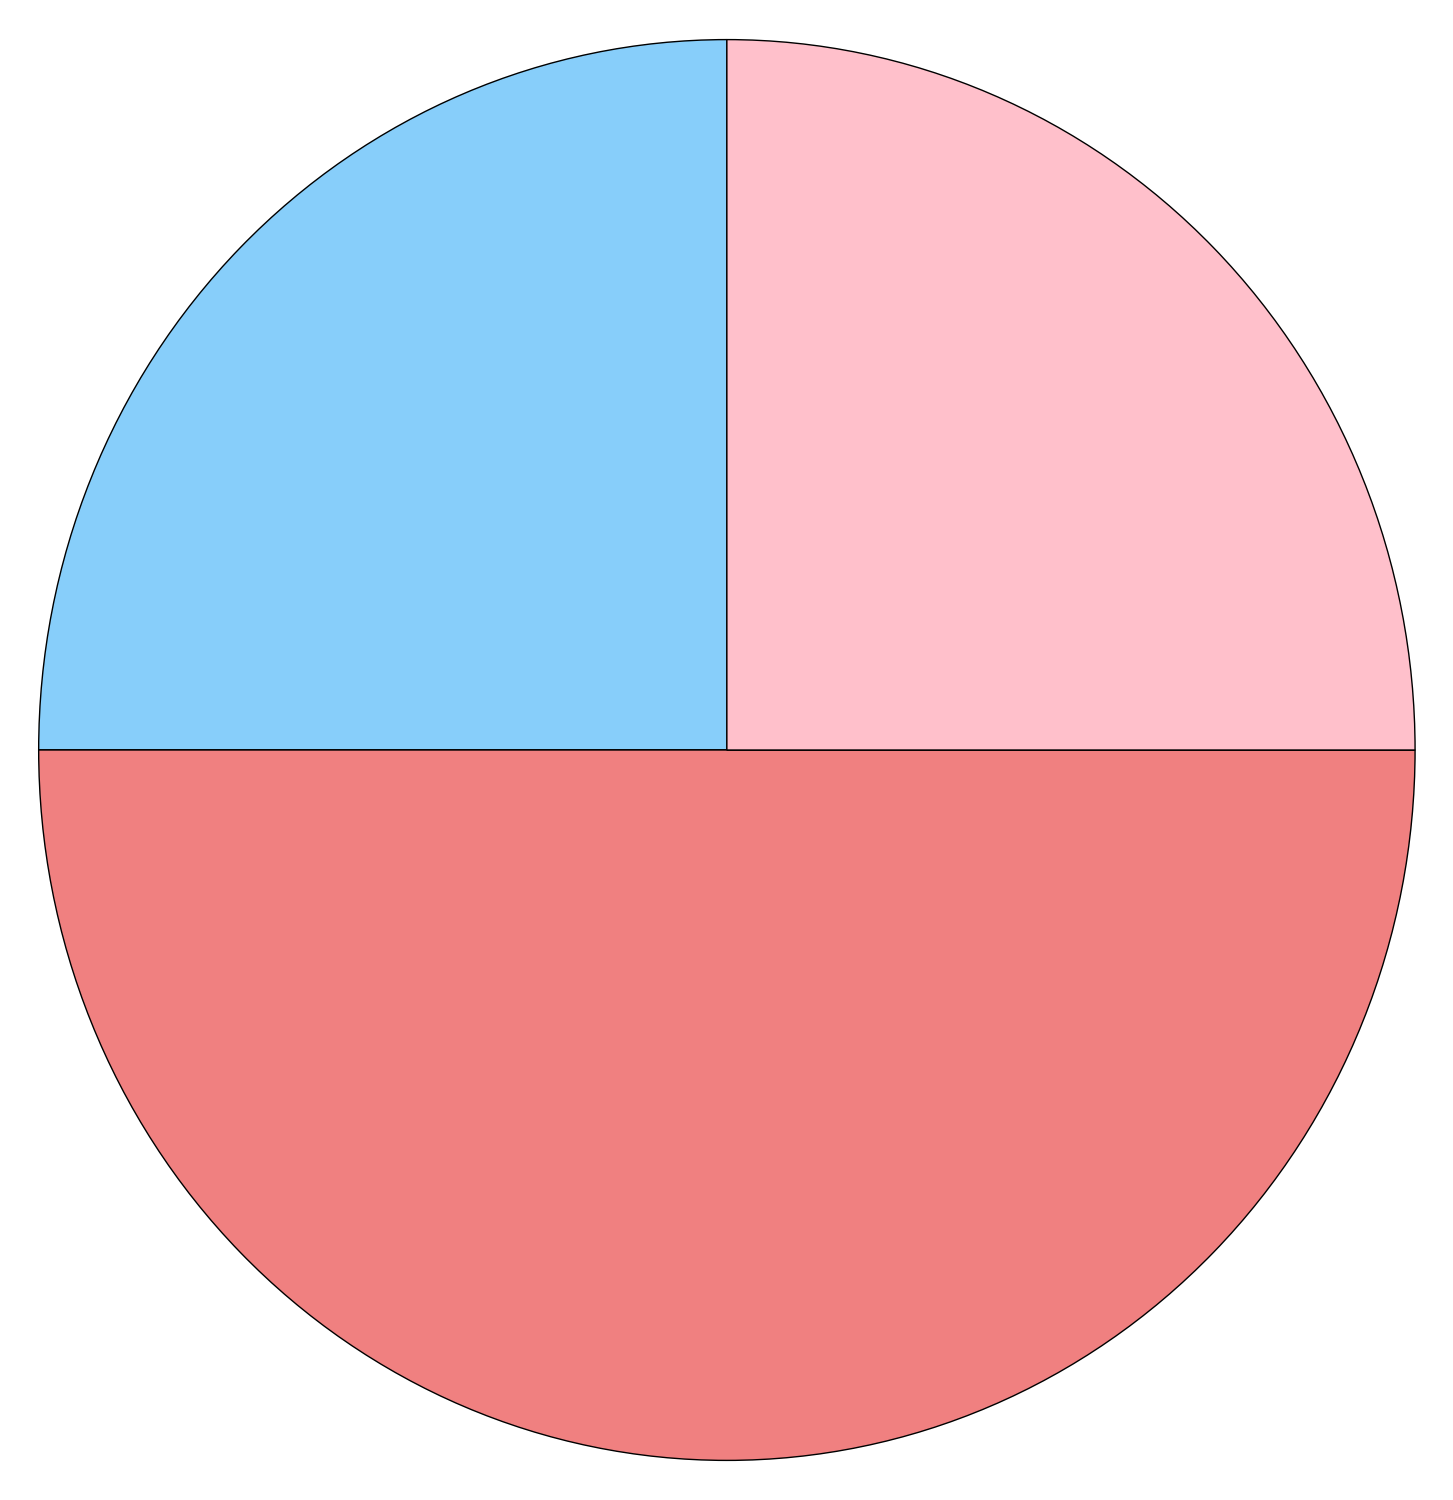
\includegraphics[width=\textwidth]{valencenon-EEGpearsonRgen}
    \caption{Pearson correlation}
  \end{subfigure}
  \hfill
  \begin{subfigure}[b]{0.3\textwidth}
    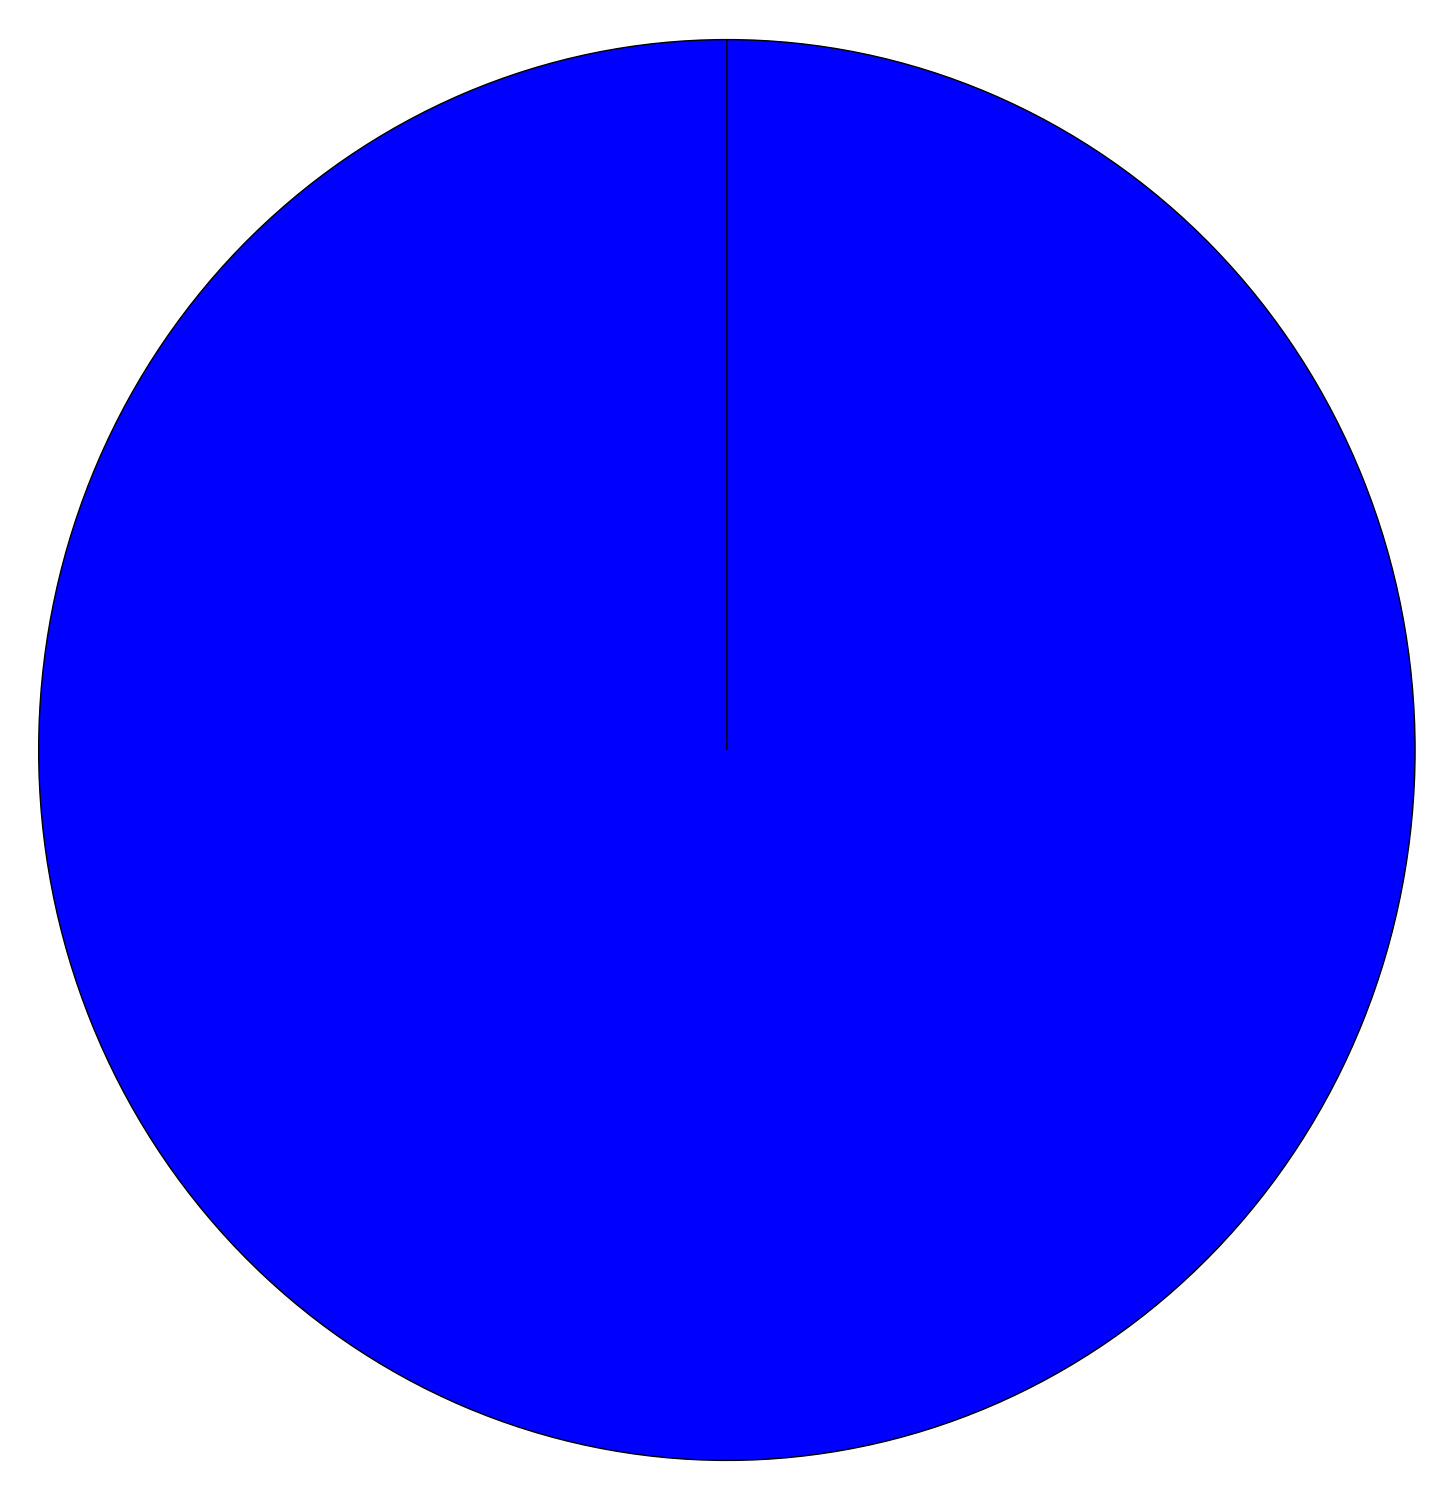
\includegraphics[width=\textwidth]{valencenon-EEGMutInfgen}
    \caption{Mutual information}
  \end{subfigure}
  \hfill
  \begin{subfigure}[b]{0.3\textwidth}
    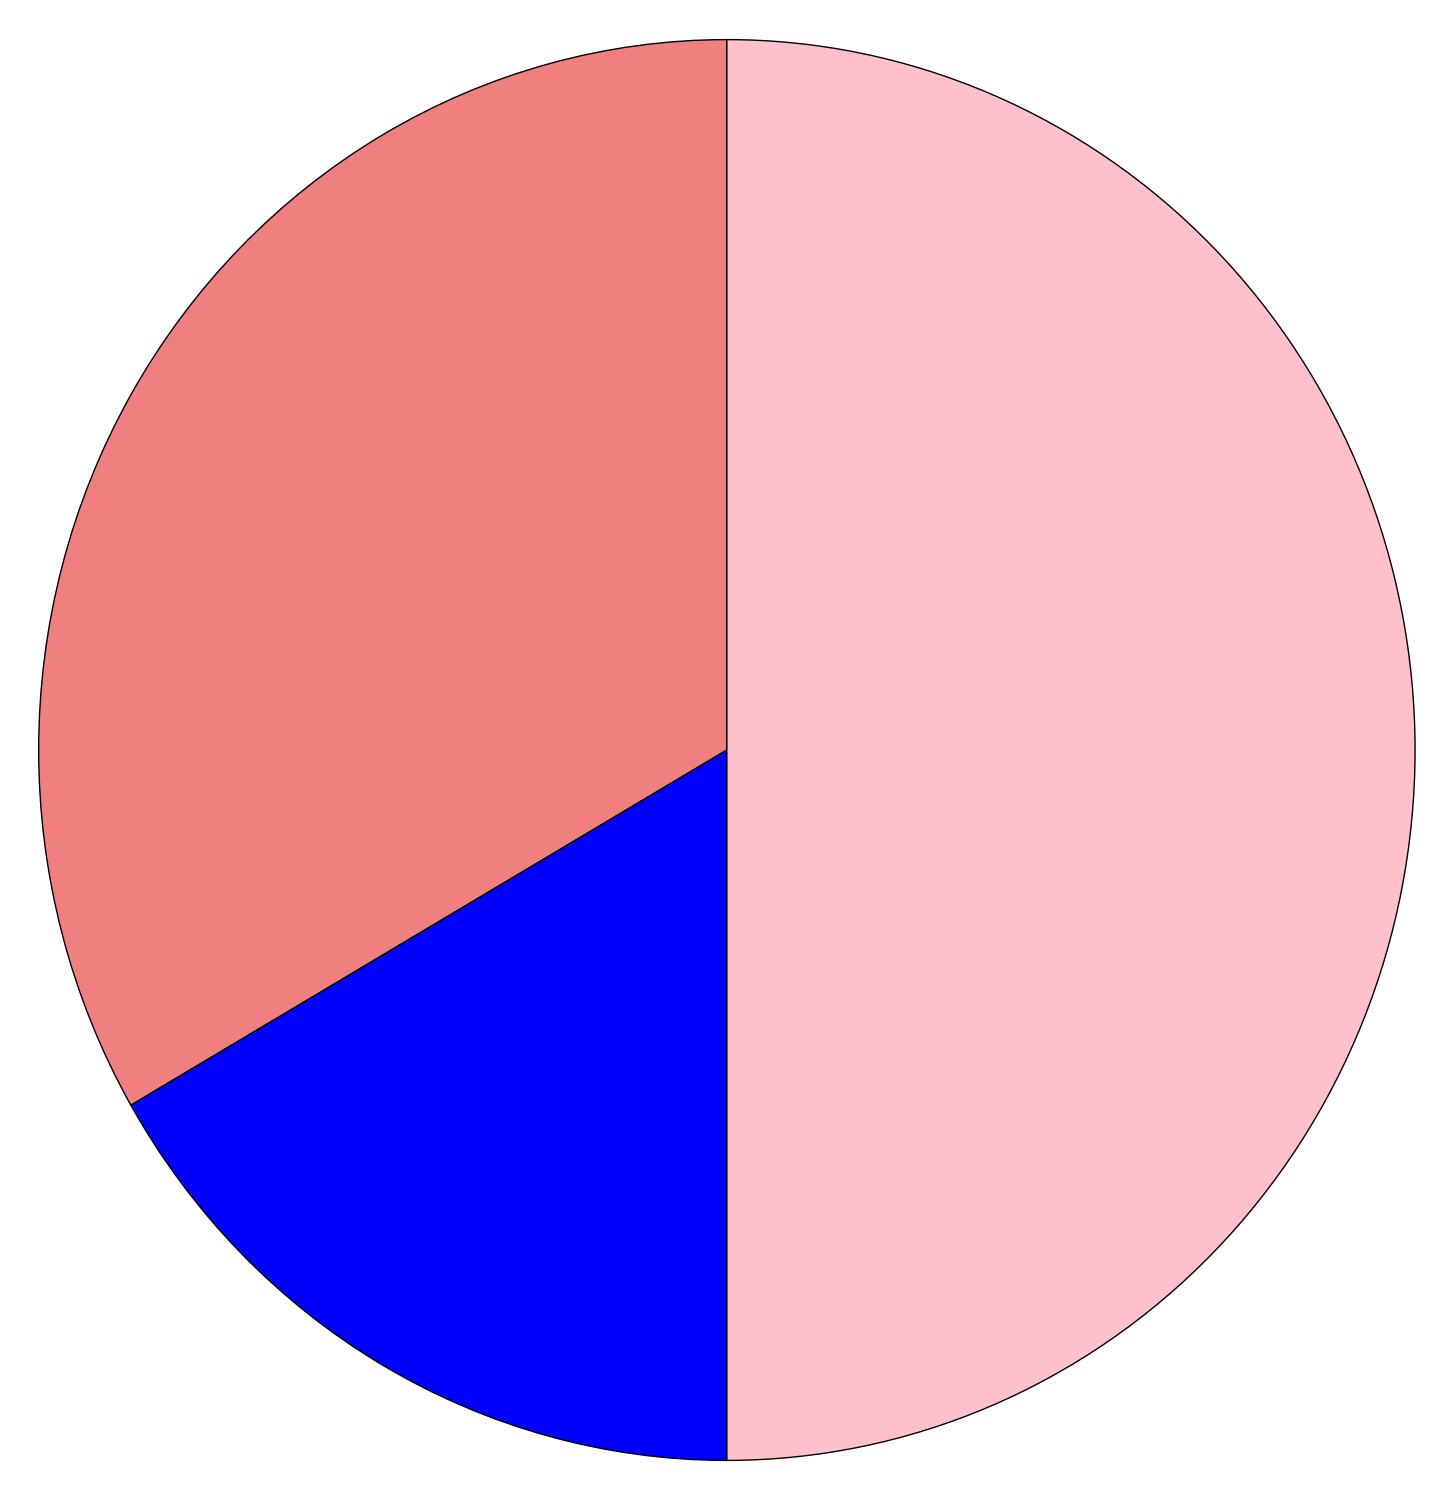
\includegraphics[width=\textwidth]{valencenon-EEGdCorrgen}
    \caption{Distance Correlation}
  \end{subfigure}
  
  \begin{subfigure}[b]{0.3\textwidth}
    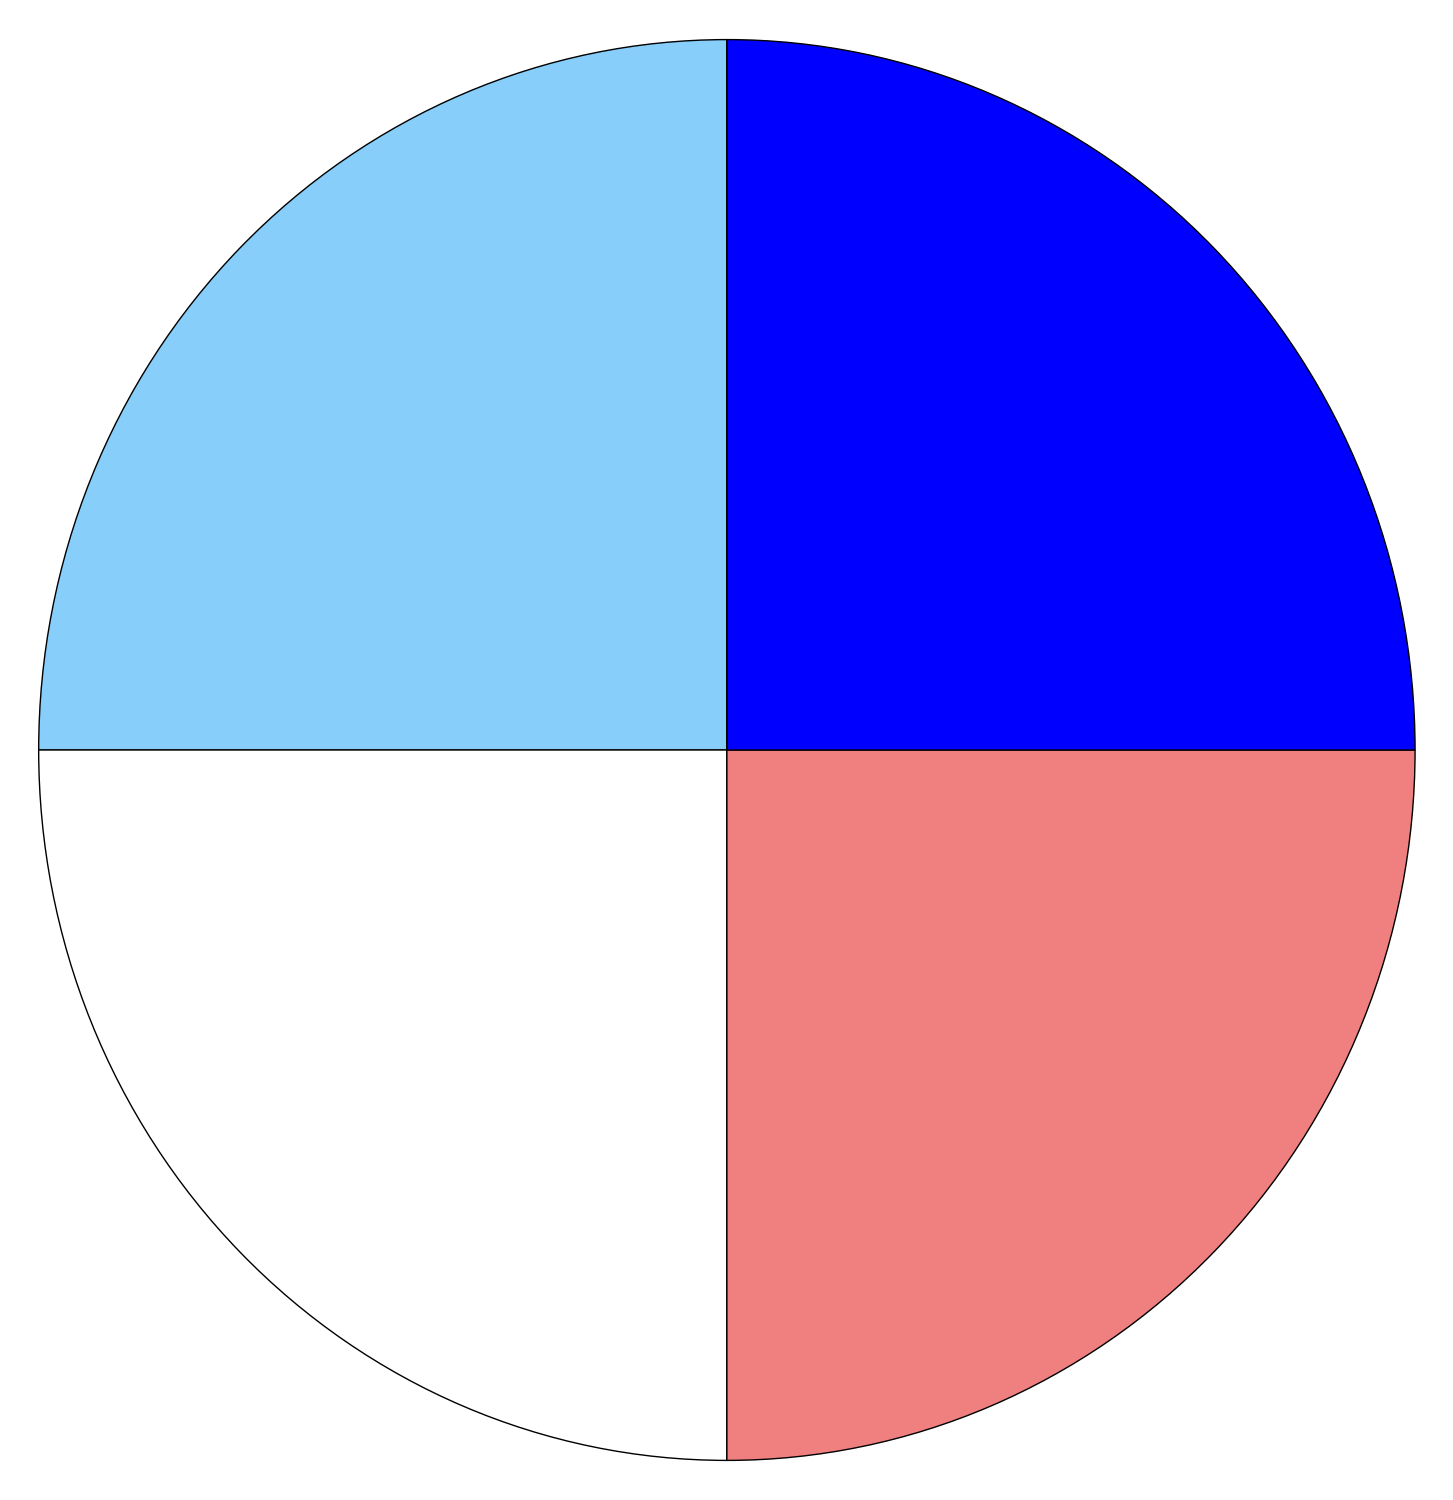
\includegraphics[width=\textwidth]{valencenon-EEGANOVAgen}
    \caption{ANOVA}
  \end{subfigure}
  \hfill
  \begin{subfigure}[b]{0.3\textwidth}
    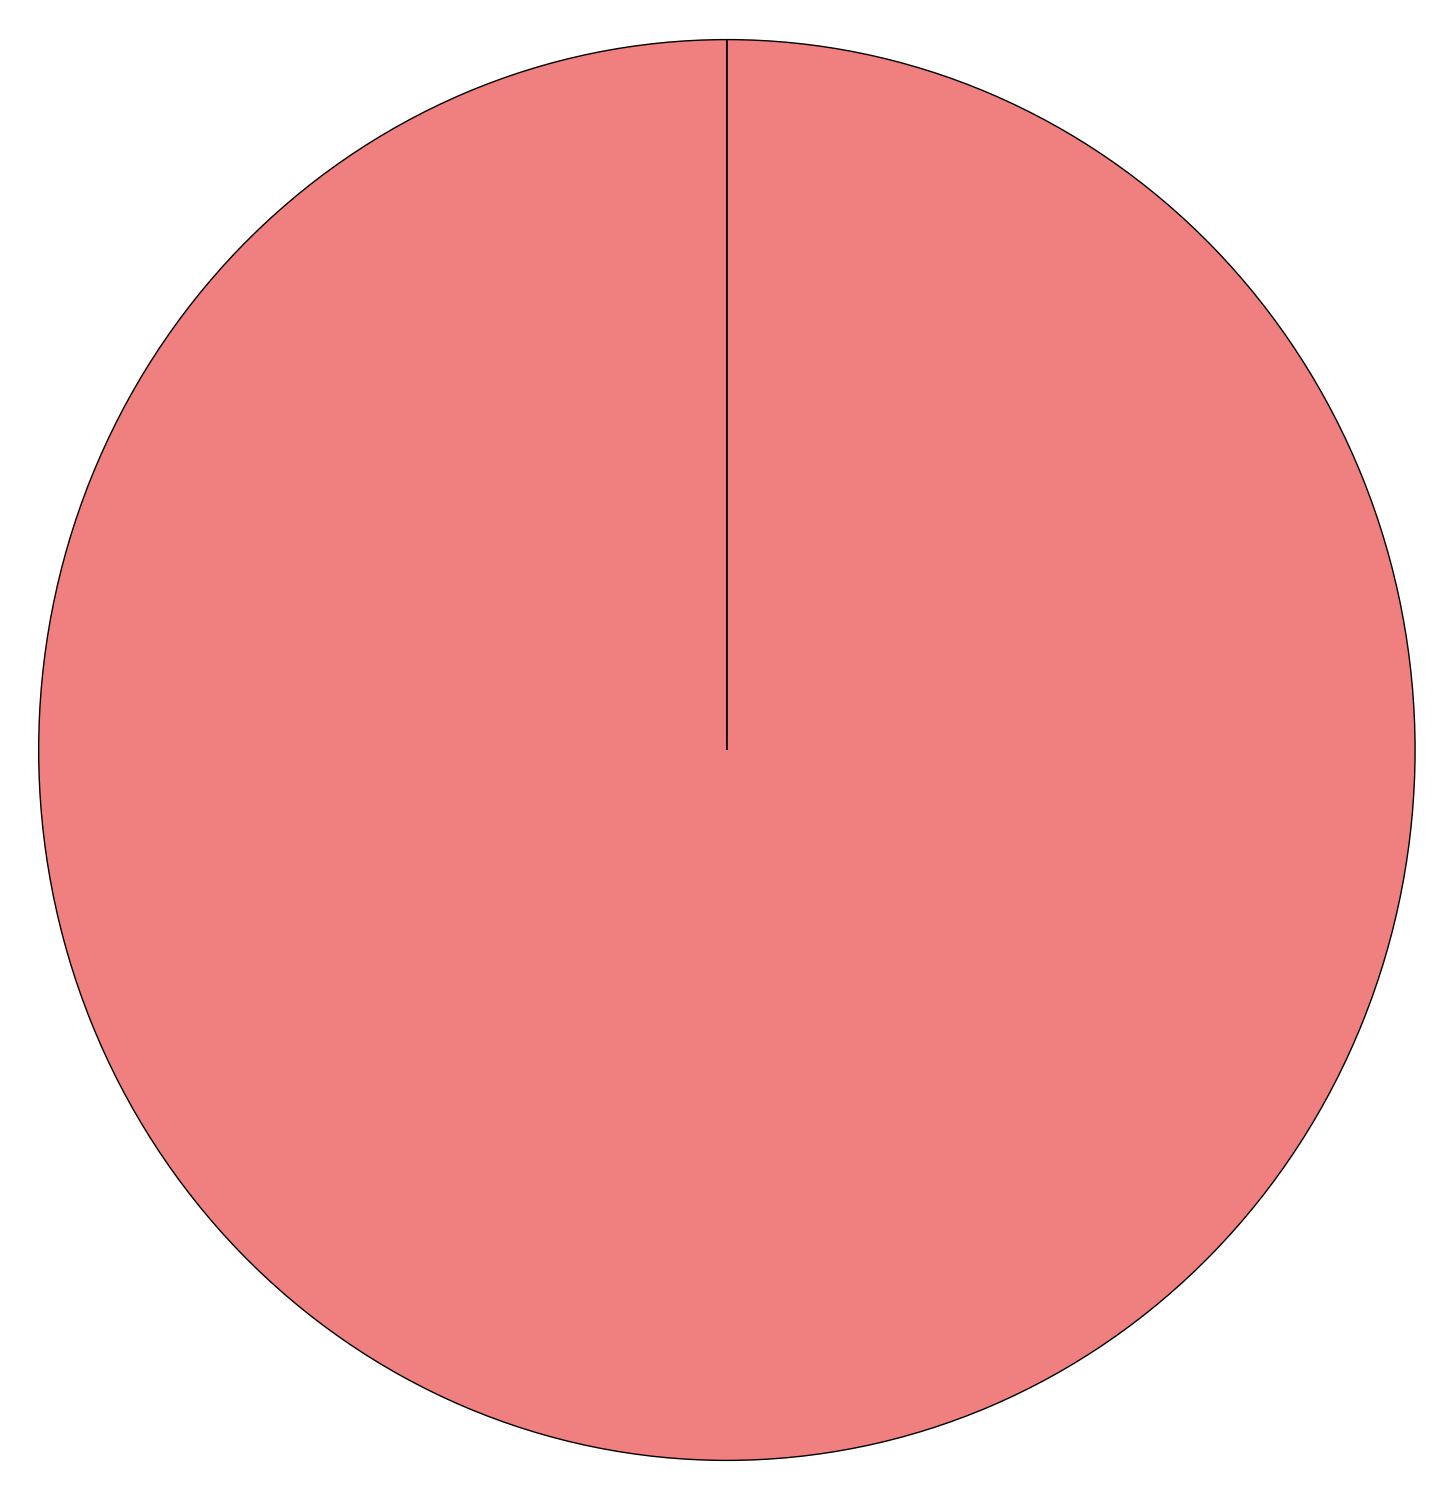
\includegraphics[width=\textwidth]{valencenon-EEGLRgen}
    \caption{Linear regression}
  \end{subfigure}
  \hfill
  \begin{subfigure}[b]{0.3\textwidth}
    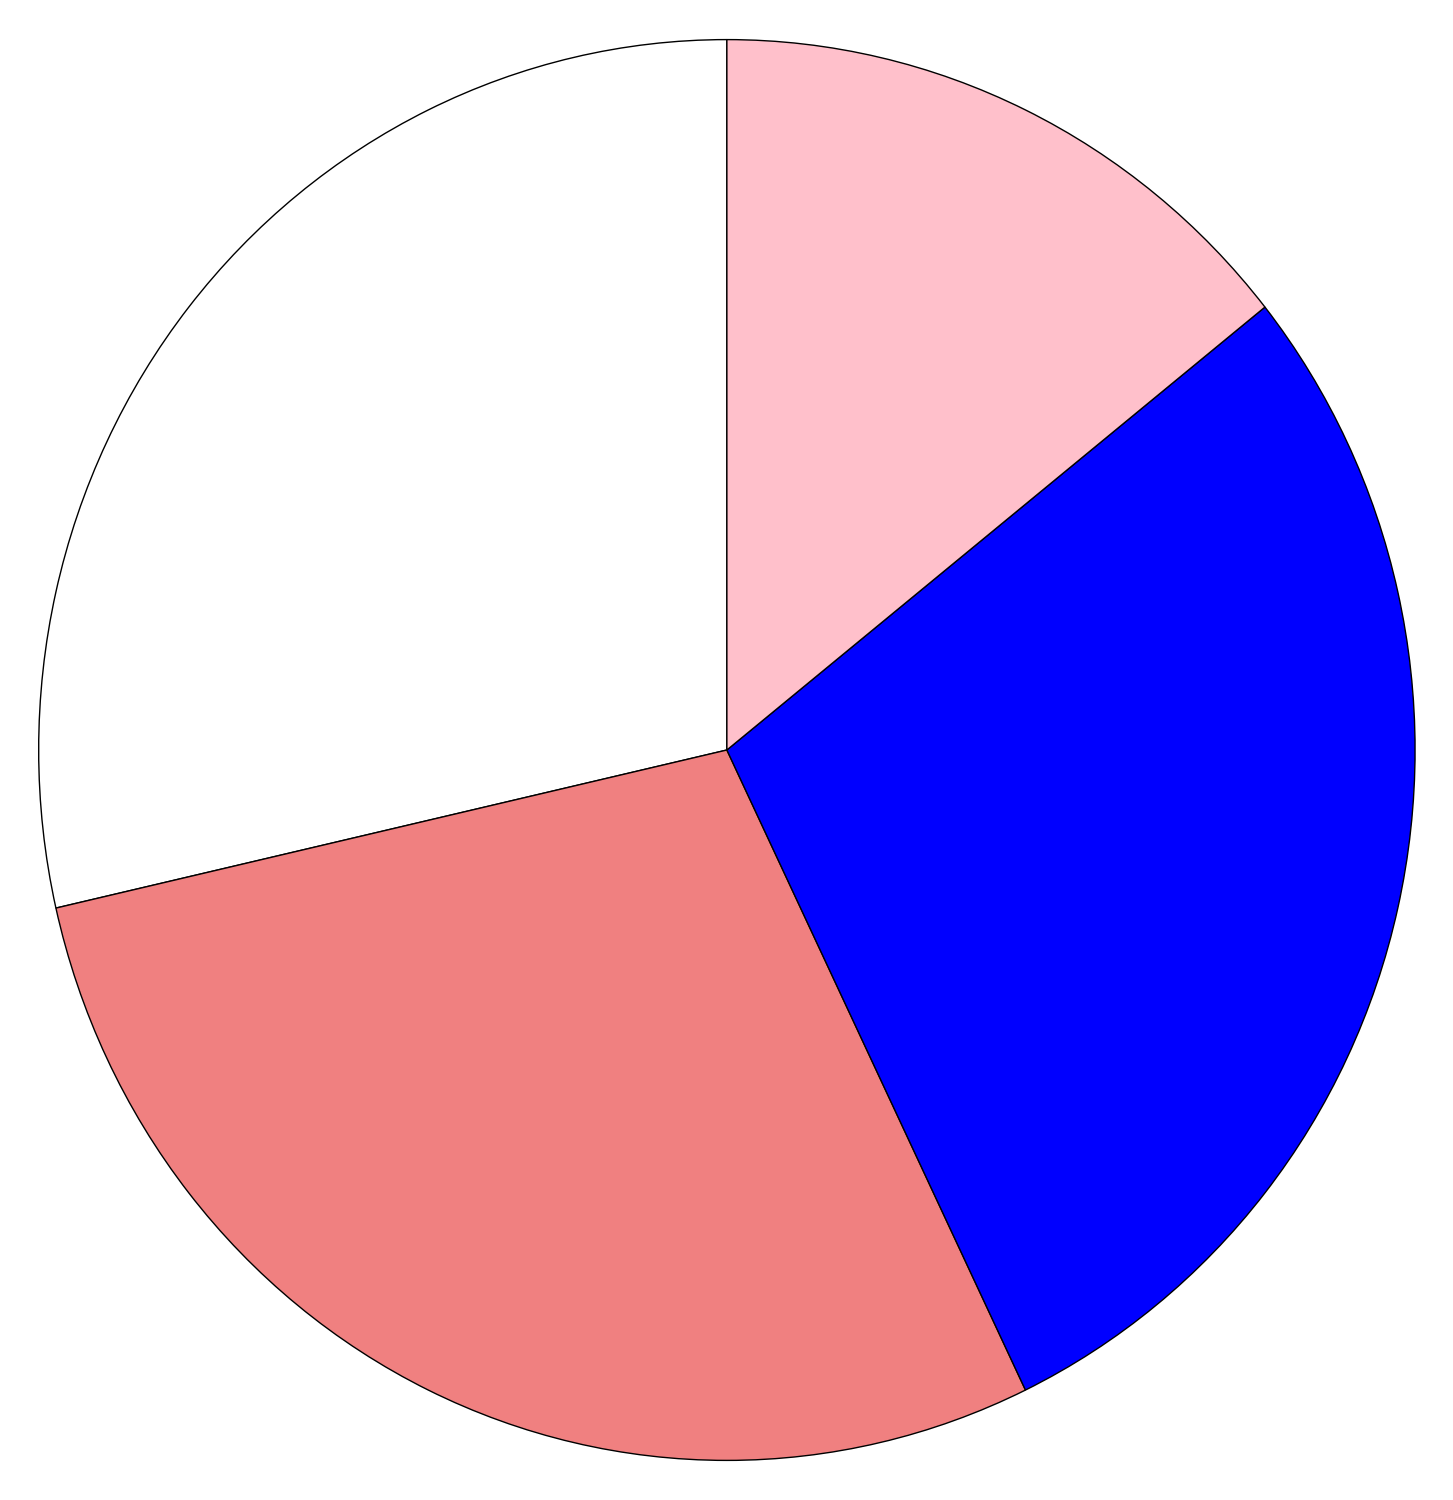
\includegraphics[width=\textwidth]{valencenon-EEGSVMgen}
    \caption{SVM}
  \end{subfigure}
  
  \begin{subfigure}[b]{0.3\textwidth}
    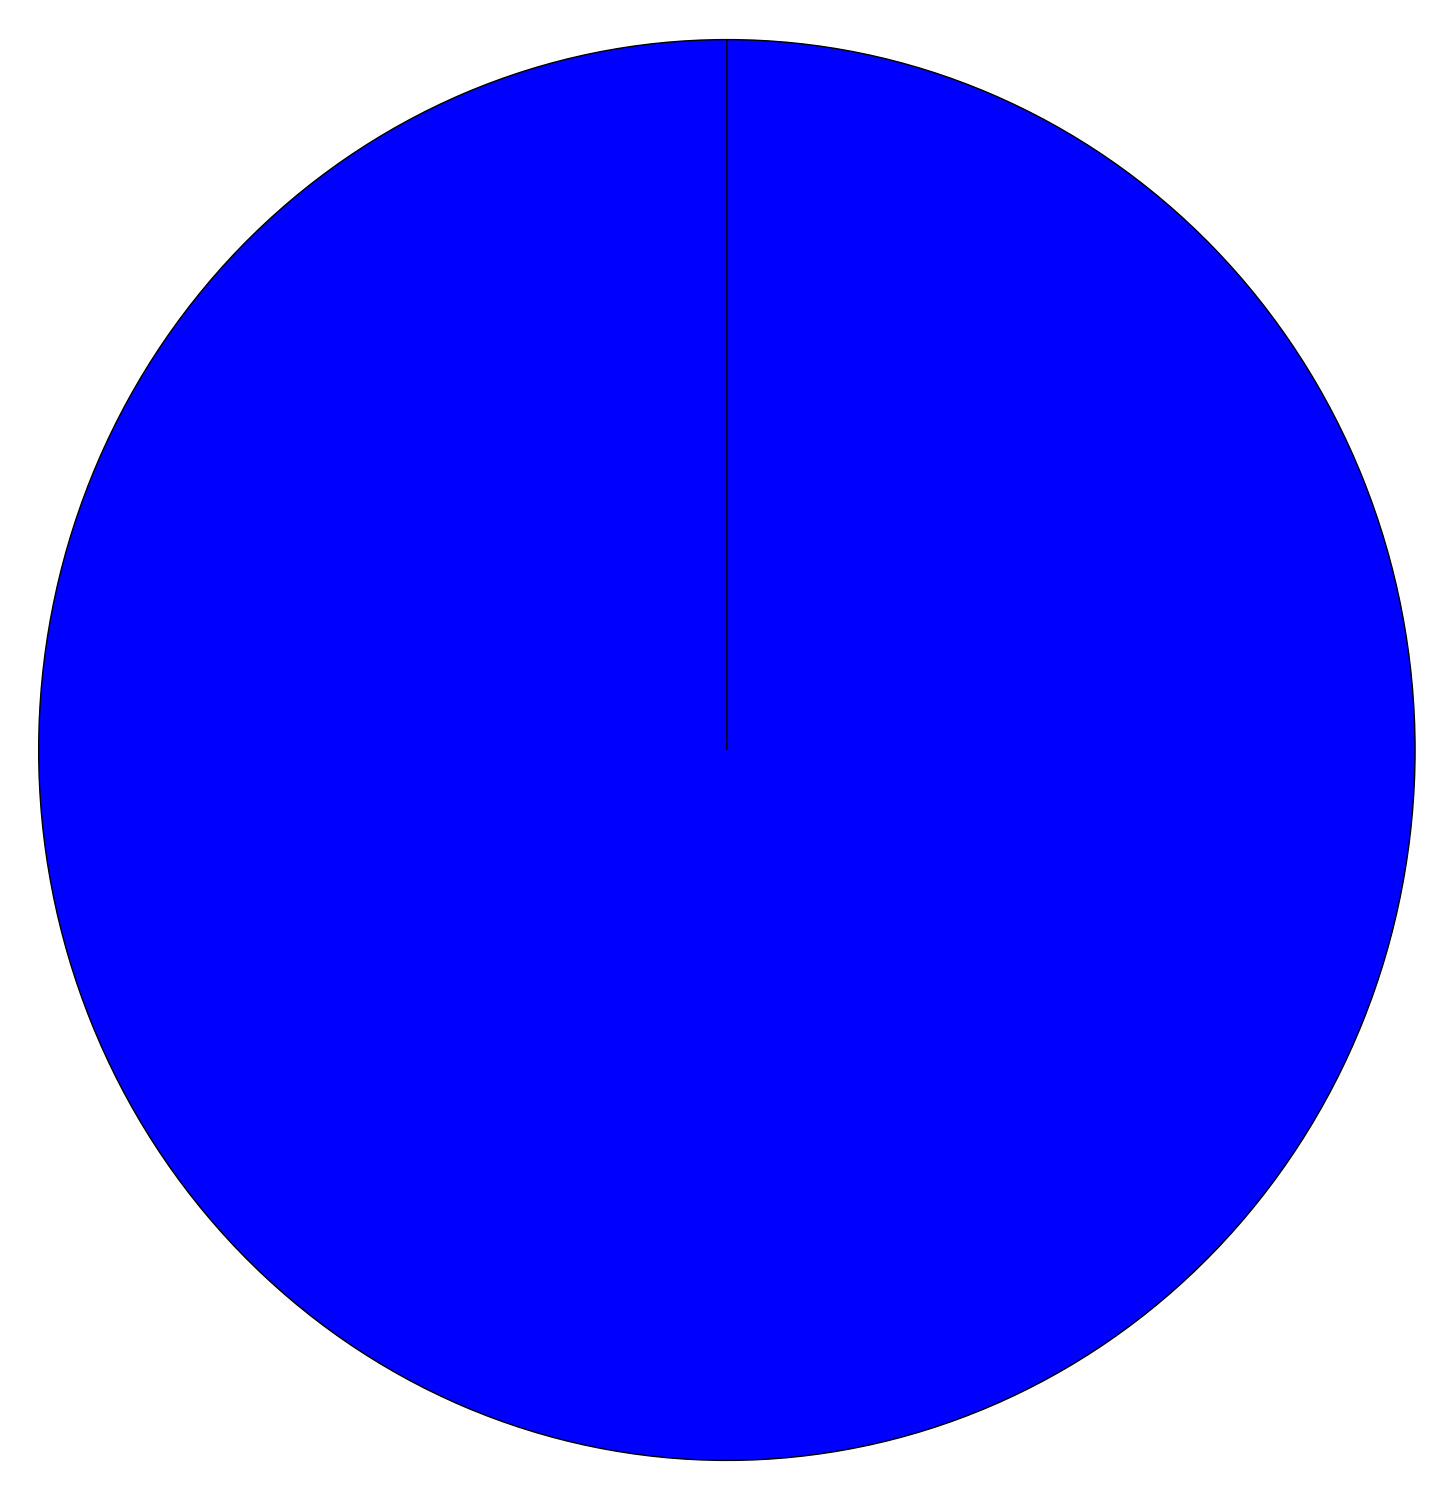
\includegraphics[width=\textwidth]{valencenon-EEGLDAgen}
    \caption{LDA}
  \end{subfigure}
  \hfill
  \begin{subfigure}[b]{0.3\textwidth}
    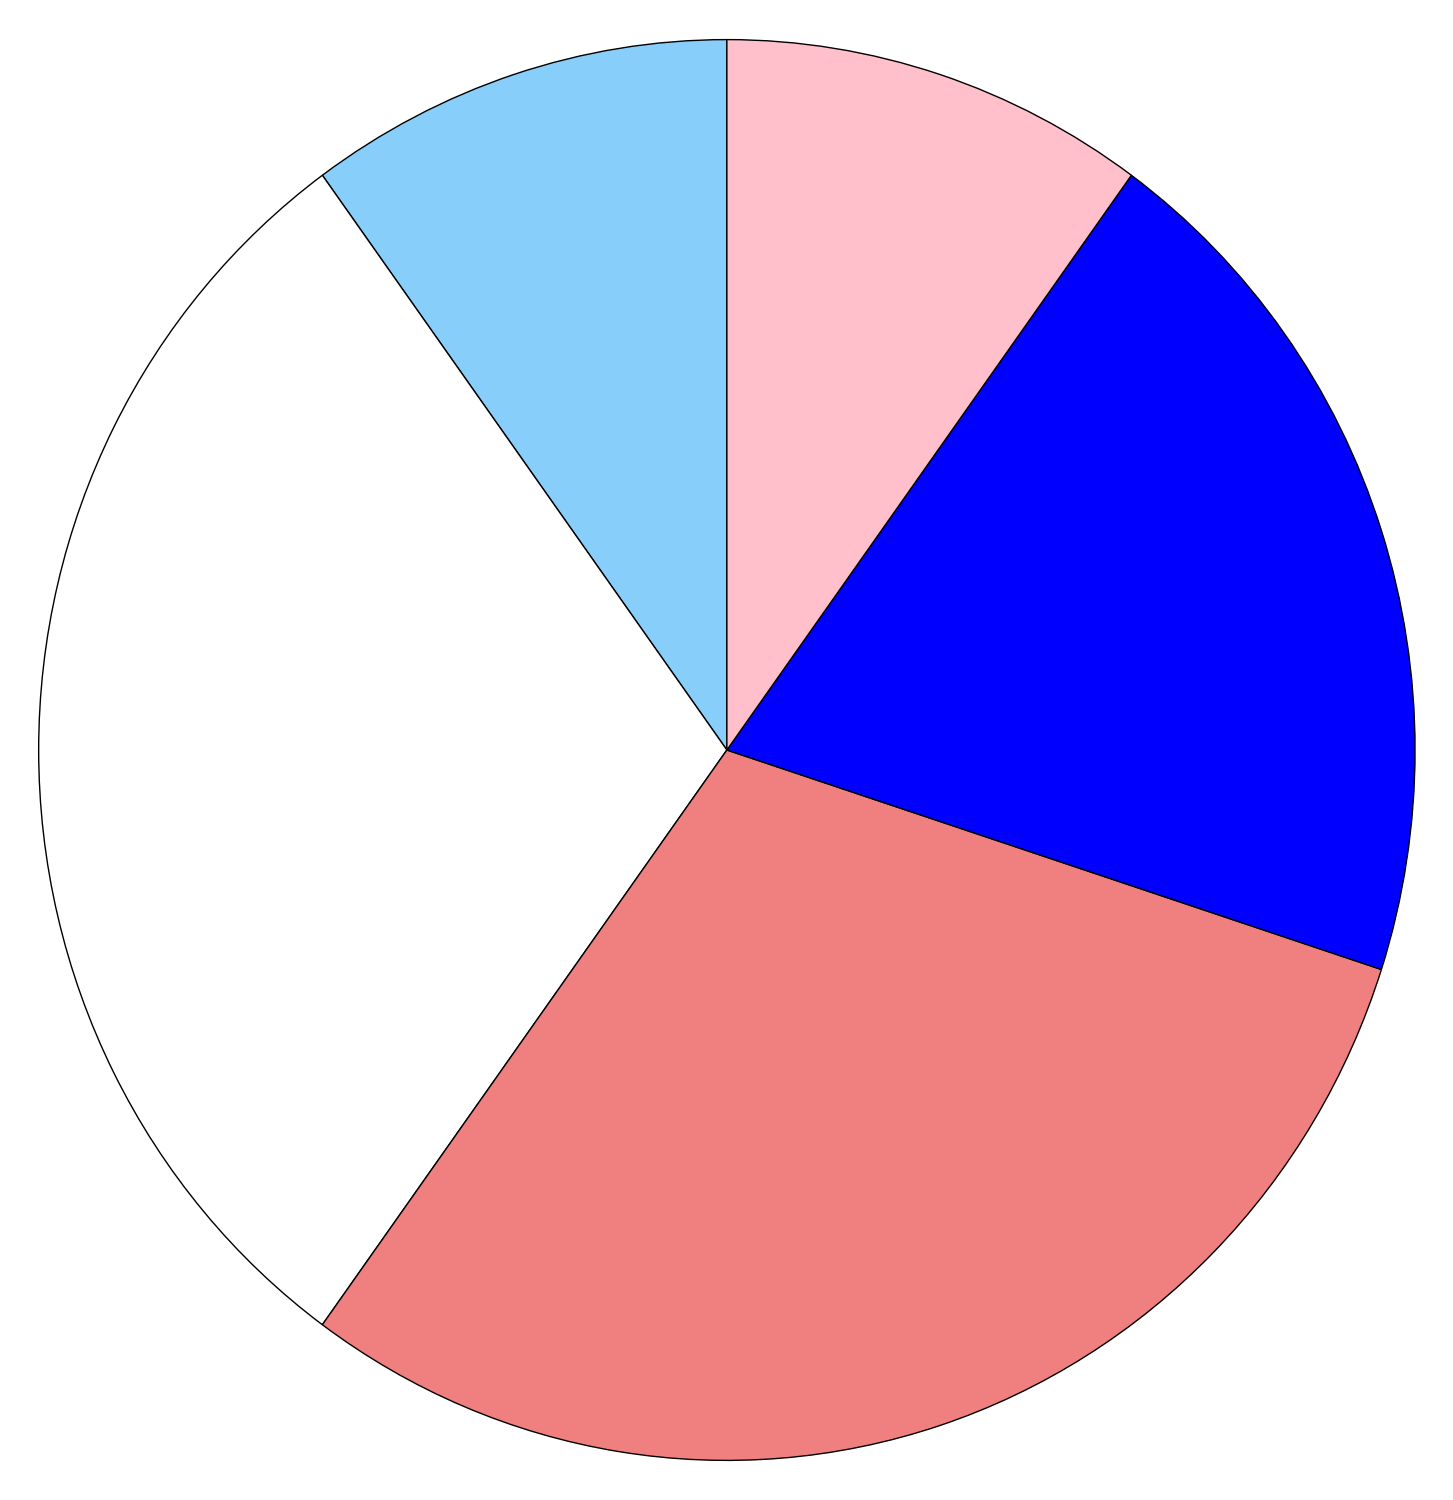
\includegraphics[width=\textwidth]{valencenon-EEGL1gen}
    \caption{Lasso regression}
  \end{subfigure}
  \hfill
  \begin{subfigure}[b]{0.3\textwidth}
    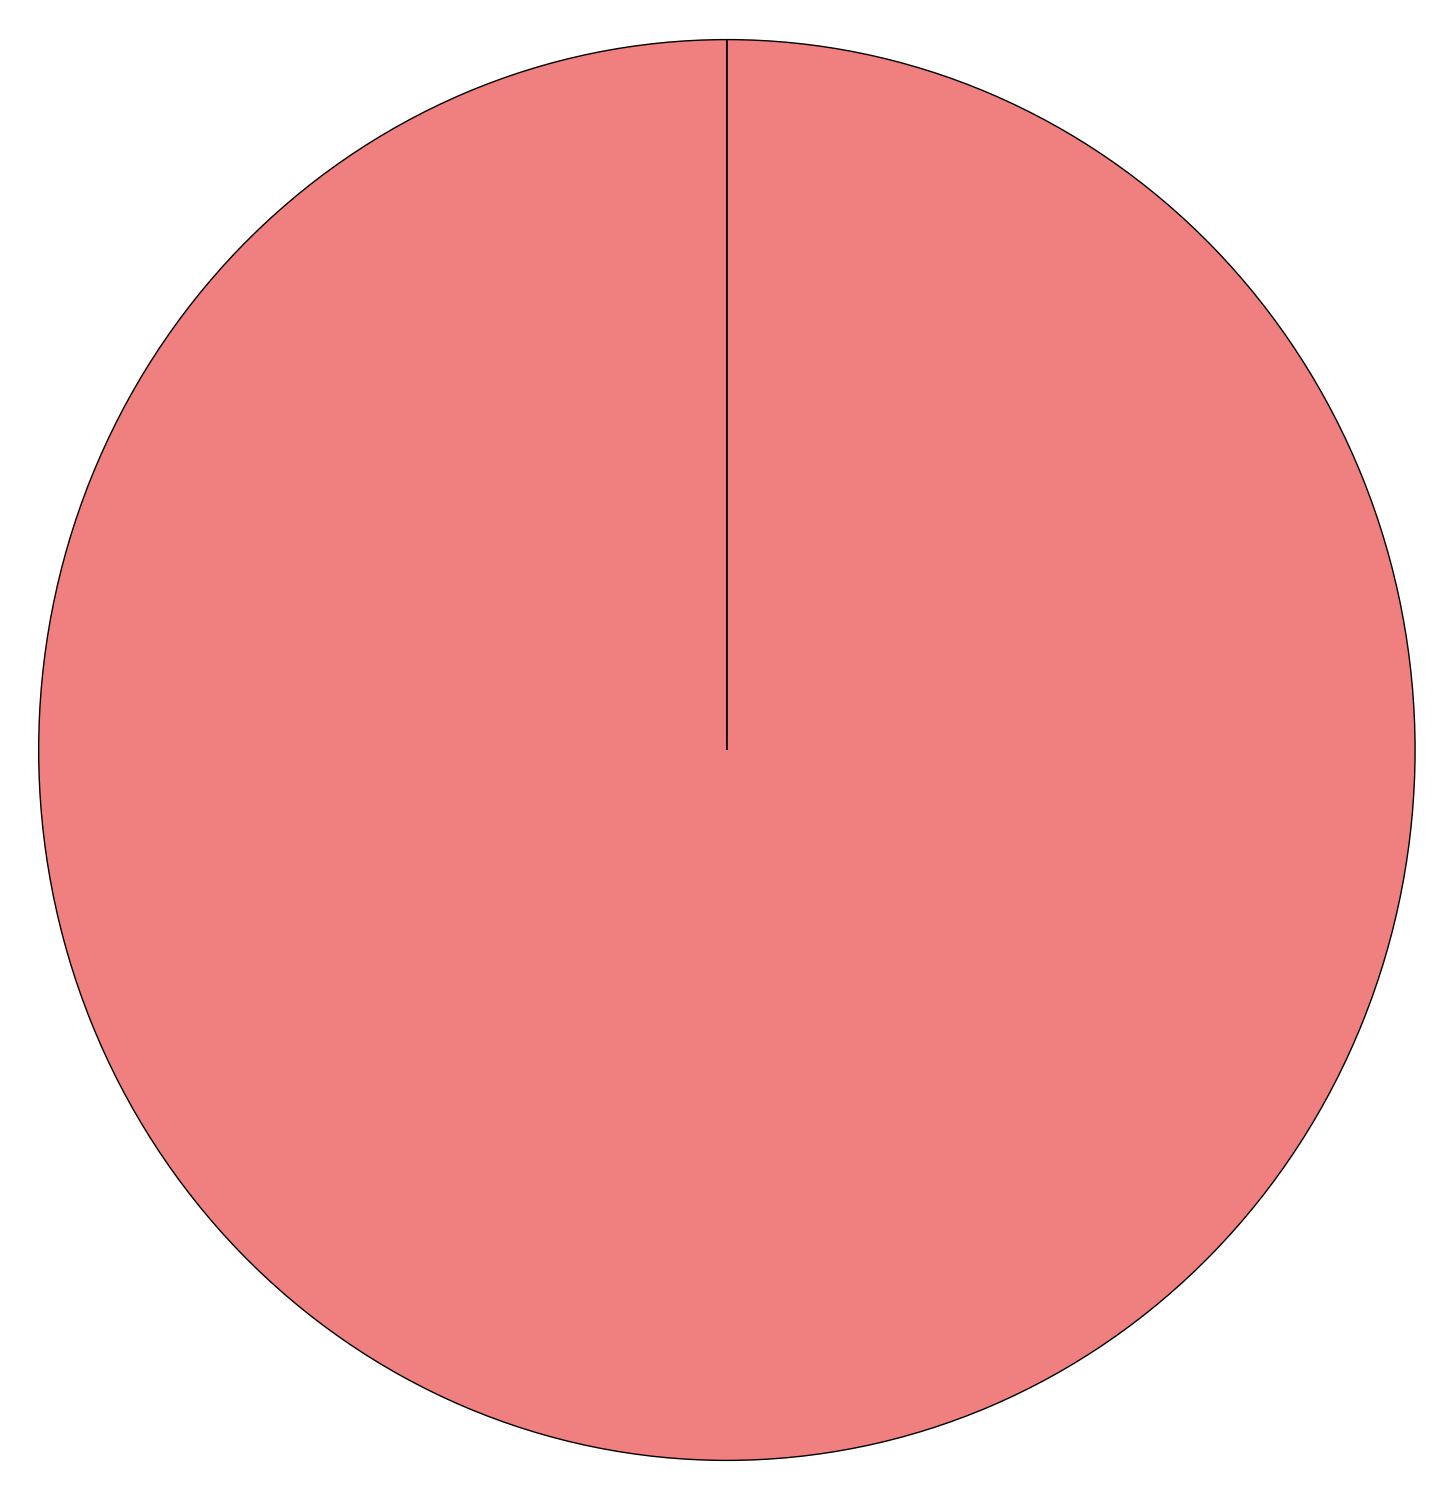
\includegraphics[width=\textwidth]{valencenon-EEGL2gen}
    \caption{Ridge regression}
  \end{subfigure}
  
  \begin{subfigure}[b]{0.3\textwidth}
    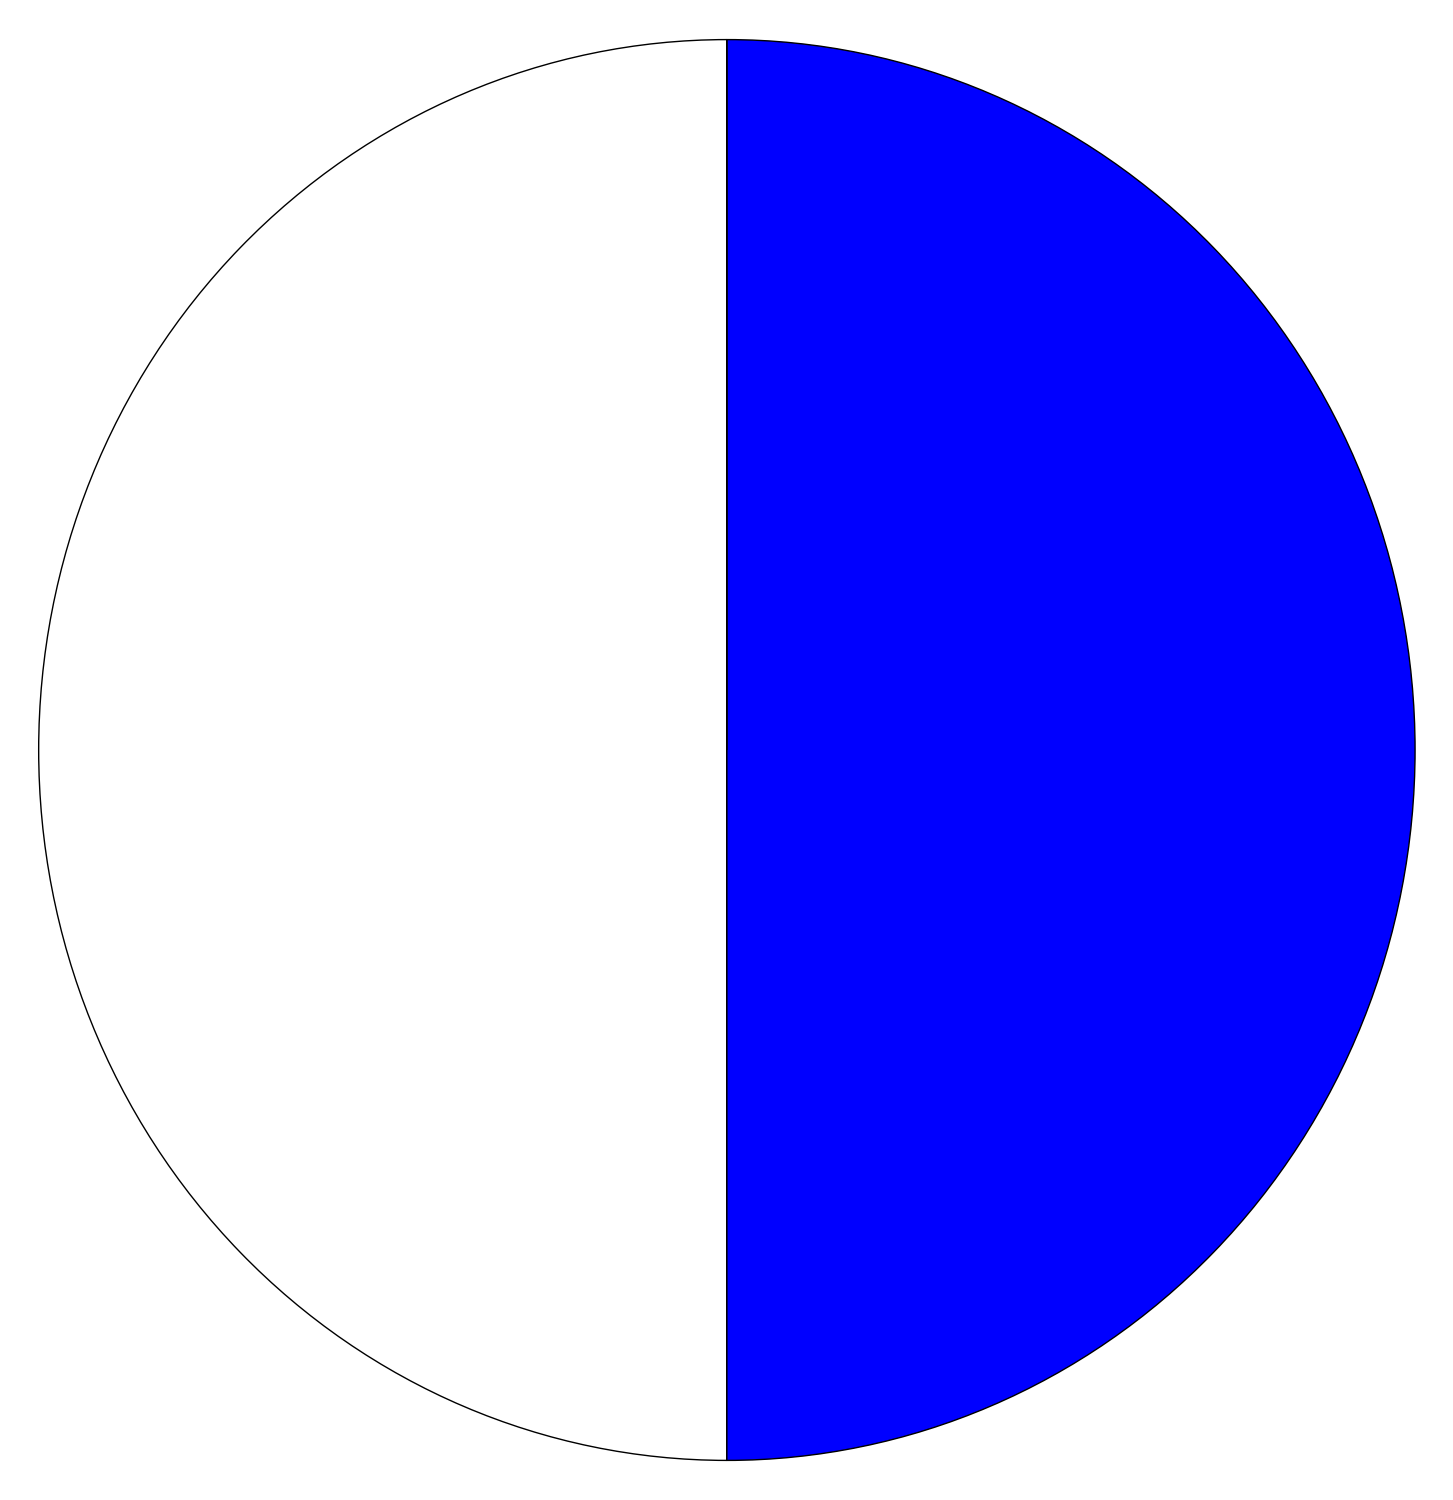
\includegraphics[width=\textwidth]{valencenon-EEGRFgen}
    \caption{Random forests}
  \end{subfigure}
  \hfill
  \begin{subfigure}[b]{0.3\textwidth}
    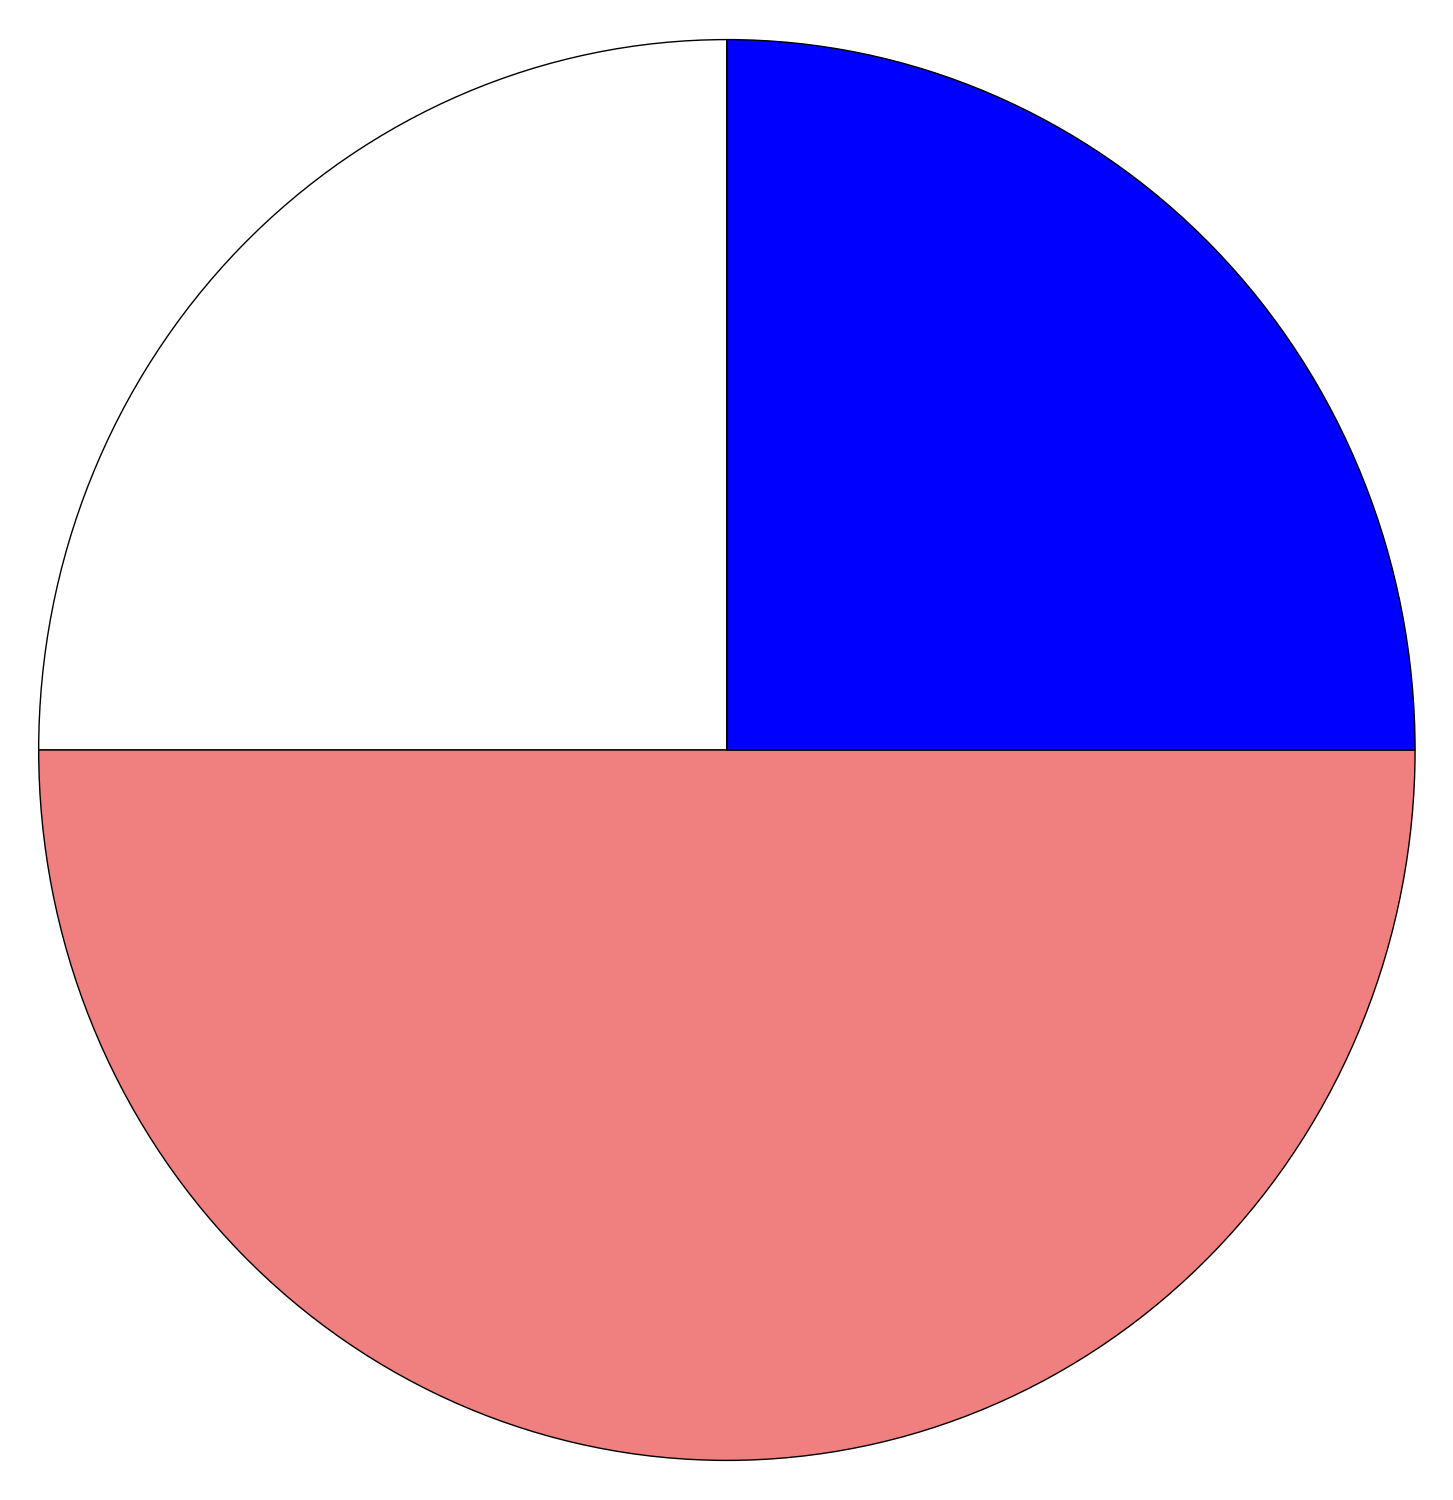
\includegraphics[width=\textwidth]{valencenon-EEGPCAgen}
    \caption{PCA}
  \end{subfigure}
  \hfill
  \begin{subfigure}[b]{0.3\textwidth}
    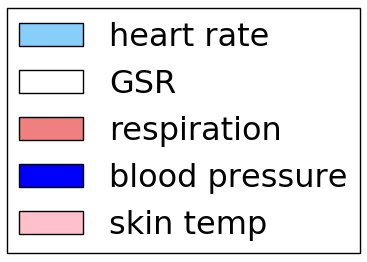
\includegraphics[width=\textwidth]{non-EEGlegend}
    \caption{Legend\label{valencepiesnon-EEGlegendgen}}
  \end{subfigure}
\end{figure}
\clearpage

\section{Important EEG channels}

\section{Stability}
TODO
%TODO